\documentclass[
    12pt,
    DIV=calc, % Anpassen für endgültige Randbreite
    BCOR=10mm, % 10mm Bindekorrektur
    ngerman,
    a4paper,
    oneside, % Einseitiges Dokument
    titlepage,
    parskip=half, % Halbe Zeile Abstand zwischen Absätzen
    headings=normal, % Größe der Überschriften
    listof=totoc, % Abbildungs- und Tabellenverzeichnis in das Inhaltsverzeichnis
    bibliography=totoc, % Literaturverzeichnis in das Inhaltsverzeichnis
    index=totoc, % Stichwortverzeichnis in das Inhaltsverzeichnis
    % captions=tableheading, % Tabellentitel als Überschriften formatieren
    % numbers=noenddot, % Überschriftnummerierung ohne Punkt
    % overfullrule=on, % Aktiviert die visuelle Hilfe für überlange Zeilen
    final % Dokumentenstatus (draft/final) (draft kann zu Inkompatibilitäten führen)
]{scrreprt}

% Sonderzeichen direkt aus dem Quelltext verwenden + Trennung von Worten mit Umlauten
\usepackage[utf8]{inputenc} 

% Allgemeine Dokumentinformationen

\title{Projekt Dokumentation}
\date{\today}
\author{Projektgruppe RIO}

\newcommand{\ctitle}{Dokumentation}
\newcommand{\csubtitle}{Teil II}
\newcommand{\cdocname}{Entwicklerhandbuch}
\newcommand{\cauthor}{Projektgruppe RIO}
\newcommand{\cdate}{\today}

% Packages für dieses Dokument
% Sprachen
\usepackage{csquotes}
\usepackage[ngerman]{babel} % Sprache festlegen

% Kopf und Fußzeilen
\usepackage[
    automark, % Kapitelangaben in Kopfzeile automatisch erstellen
    headsepline, % Trennlinie unter Kopfzeile
    footsepline, % Trennlinie über Fußzeile
    ilines % Trennlinie linksbündig ausrichten
]{scrlayer-scrpage}

%% Für \makeglossaries
%\usepackage{makeidx}

% Schriften und Zeichenencodierung
\usepackage[T1]{fontenc} % Für < und > im Text
\usepackage{lmodern} % Scalable Font für microtype
\usepackage{textcomp} % Für ° Zeichen über \textdegree
\usepackage{amsmath} % Math-Umgebung im Text
\usepackage{siunitx} % Units in Math und Text-Umgebungen
\usepackage[gen]{eurosym} % official für immer das selbe € Symbol, gen für Anpassungen (Kursiv, etc)
\usepackage{microtype} % Wortumbrechungen verringern

\ifcsname{counterwithout}\endcsname%
%
\else%
%\usepackage{chngcntr} % Für \counterwithout auf Windows
\fi%

% Fußnoten auch bei Verwendung von hyperref
\usepackage{footnotehyper}

\usepackage{setspace}
\usepackage[
	%showframe, % Seitenlayout anzeigen, auskommentieren für finales Dokument
	left=25mm,
	right=25mm,
	top=25mm,
	bottom=25mm,
	includeheadfoot
]{geometry}

\usepackage{pdflscape} % Für gedrehte Seiten in der PDF.

\usepackage{xcolor} % Farbboxen im Text
\definecolor{mygreen}{rgb}{0,0.6,0}
\definecolor{mygray}{rgb}{0.5,0.5,0.5}
\definecolor{mymauve}{rgb}{0.58,0,0.82}

\usepackage{listings} % Code-Ausschnitte
% Formatierung von Listings
\lstset{ %
  float=hbp,
  backgroundcolor=\color{white},   % choose the background color; you must add \usepackage{color} or \usepackage{xcolor}
  %basicstyle=\footnotesize,        % the size of the fonts that are used for the code
    basicstyle=\ttfamily\color{black}\small, %\smaller,
  breakatwhitespace=false,         % sets if automatic breaks should only happen at whitespace
  breaklines=true,                 % sets automatic line breaking
    breakautoindent=true,
  captionpos=b,                    % sets the caption-position to bottom
    columns=flexible,
    tabsize=2,
    frame=false,
  commentstyle=\color{mygreen},    % comment style
  deletekeywords={...},            % if you want to delete keywords from the given language
  escapeinside={(*@}{@*)},          % if you want to add LaTeX within your code
  extendedchars=true,              % lets you use non-ASCII characters; for 8-bits encodings only, does not work with UTF-8
  %frame=single,                    % adds a frame around the code
  keepspaces=true,                 % keeps spaces in text, useful for keeping indentation of code (possibly needs columns=flexible)
  keywordstyle=\color{blue},       % keyword style
  morekeywords={*,...},            % if you want to add more keywords to the set
    emph={decltype,string,constexpr,static_assert},
    emphstyle=\color{blue},
    emph=[2]{NULL,nullptr},
    emphstyle=[2]\color{mymauve},
  numbers=left,                    % where to put the line-numbers; possible values are (none, left, right)
  numbersep=5pt,                   % how far the line-numbers are from the code
  numberstyle=\tiny\color{mygray}, % the style that is used for the line-numbers
  rulecolor=\color{black},         % if not set, the frame-color may be changed on line-breaks within not-black text (e.g. comments (green here))
  showspaces=false,                % show spaces everywhere adding particular underscores; it overrides 'showstringspaces'
  showstringspaces=false,          % underline spaces within strings only
  showtabs=false,                  % show tabs within strings adding particular underscores
  stepnumber=1,                    % the step between two line-numbers. If it's 1, each line will be numbered
  stringstyle=\color{mygreen},     % string literal style
  tabsize=2                        % sets default tabsize to 2 spaces
  %title=\lstname                   % show the filename of files included with \lstinputlisting; also try caption instead of title
}

\usepackage{bera}% optional: just to have a nice mono-spaced font

\colorlet{punct}{red!60!black}
\definecolor{background}{HTML}{EEEEEE}
\definecolor{delim}{RGB}{20,105,176}
\colorlet{numb}{magenta!60!black}

\lstdefinelanguage{json}{
	basicstyle=\normalfont\ttfamily,
	numbers=left,
	numberstyle=\scriptsize,
	stepnumber=1,
	numbersep=8pt,
	showstringspaces=false,
	breaklines=true,
	frame=lines,
	backgroundcolor=\color{background},
	literate=
	*{0}{{{\color{numb}0}}}{1}
	{1}{{{\color{numb}1}}}{1}
	{2}{{{\color{numb}2}}}{1}
	{3}{{{\color{numb}3}}}{1}
	{4}{{{\color{numb}4}}}{1}
	{5}{{{\color{numb}5}}}{1}
	{6}{{{\color{numb}6}}}{1}
	{7}{{{\color{numb}7}}}{1}
	{8}{{{\color{numb}8}}}{1}
	{9}{{{\color{numb}9}}}{1}
	{:}{{{\color{punct}{:}}}}{1}
	{,}{{{\color{punct}{,}}}}{1}
	{\{}{{{\color{delim}{\{}}}}{1}
	{\}}{{{\color{delim}{\}}}}}{1}
	{[}{{{\color{delim}{[}}}}{1}
	{]}{{{\color{delim}{]}}}}{1},
}

\usepackage{appendix} % Anhang

\usepackage[german]{fancyref}
\fancyrefchangeprefix{\fancyrefchaplabelprefix}{cha}
\fancyrefchangeprefix{\fancyreftablabelprefix}{tbl}

\usepackage[final]{graphicx} % Einbinden von jpeg-Dateien

% \usepackage{awesomebox} % Für Infoboxen (benötigt XeLaTeX)
\usepackage{mdframed} % Für Infoboxen
\usepackage{afterpage} % Pages einfügen (um Floats zu flushen).
\usepackage{placeins} % Floats flushen (erzwungen).

\usepackage{placeins}
\usepackage{tikz-uml}
\usepackage{here} %großes H um Bilder an genau der Stelle zu erzwingen
\usepackage{tabularx} %für einheitliche Tabellenbreite
\usepackage{longtable} % Für tabellen über mehrere Seiten
\usepackage{tocbasic}

% Url mit Optionen vor hyperref und biblatex!
\usepackage[hyphens]{url}

% Zitieren aus Literaturverzeichnis
\usepackage[style=numeric, backend=biber]{biblatex}

% Hyperref so spät wie möglich laden, damit keine Probleme mit Verlinkungen im Dokument entstehen
\usepackage[
    bookmarks=true,
    bookmarksopen=true,
    %hyperfootnotes=false,
    hypertexnames=false,
    linktocpage=true,
    pdfpagelabels=true,
    plainpages=false,
    % Farben für finalen Druck auf black setzen
    anchorcolor=black,
    citecolor=blue,
    colorlinks=true,
    filecolor=magenta,
    linkcolor=red,
    menucolor=red,
    urlcolor=cyan
]{hyperref}

\hypersetup{
	breaklinks=true,
	final=true,
    pdftitle={\ctitle},
    pdfauthor={\cauthor},
    pdfcreator={\cauthor},
    pdfsubject={\ctitle},
    pdfkeywords={\ctitle}
}
\usepackage{array}



\makeindex

% Dokumentenstil

\onehalfspacing % Zeilenabstand 1.5


% Kopf- und Fußzeilen über KOMA-Skript
\pagestyle{scrheadings}
\renewcommand*{\chapterpagestyle}{scrheadings}
\renewcommand{\headfont}{\normalfont}

% Kopfzeile
\ihead{\large{\textsc{\ctitle}}\\ \small{\csubtitle} \\[1ex] \textit{\headmark}}
\chead{}
\ohead{
\includegraphics[scale=0.12]{ressourcen/Logo-UOL.png}}
\setlength{\headheight}{20mm} % Höhe der Kopfzeile
%\setheadwidth[0pt]{textwithmarginpar}

% Fußzeile
\ifoot{\cauthor}
\cfoot{\\}
\ofoot{\pagemark}
\setlength{\footheight}{15mm} % Höhe der Fußzeile
%\setlength{\footskip}{1cm}

% Verzeichnisse stylen
\makeatletter
\renewcommand*\@pnumwidth{2em}
\makeatother
\DeclareTOCStyleEntry[numwidth=2em]{undottedtocline}{chapter}
\DeclareTOCStyleEntry[numwidth=2.8em,indent=2em]{dottedtocline}{section}
\DeclareTOCStyleEntry[numwidth=3.2em,indent=4.8em]{dottedtocline}{subsection}
\DeclareTOCStyleEntries[numwidth=2.8em,indent=2em]{dottedtocline}{figure,table}

% Sonstiges
\frenchspacing % Mehr Platz hinter einem Punkt

% Schusterjungen und Hurenkinder vermeiden
\clubpenalty = 10000
\widowpenalty = 10000
\displaywidowpenalty = 10000

% Fußnoten fortlaufend nummerieren
\counterwithout{footnote}{chapter}

% Zeilenabstand in Mathematischen Formeln
%\setlength\jot{5mm}


% Selbst definierte Befehle für dieses Dokument 

% Mailadressen als Link einfügen
\newcommand{\mailaddr}[1]{{\href{mailto:#1}{#1}}}
% Abbildungen einfügen
\newcommand{\abb}[1]{Abbildung~\ref{#1}}
% PictureDetail Kommando um Nennungen von Bildinhalten einheitlich hervorzuheben.
\newcommand{\PicDet}[1]{\textit{#1}}

% \newcommand{\TODOpassage}[1]{\textcolor{red}{ToDo: #1}}
% \renewcommand{\TODOpassage}[1]{}
% \newcommand{\TODO}{\textcolor{red}{ToDo: }}
% \newcommand{\TODO}{}

\newcommand{\filename}[1]{\textit{#1}}
\newcommand{\dirname}[1]{\textit{#1}}
\newcommand{\reponame}[1]{\textit{#1}}
\newcommand{\console}[1]{\colorbox{lightgray}{\small\texttt{#1}}}
\newcommand{\code}[1]{\colorbox{lightgray}{\small\texttt{#1}}}

\newcommand{\pg}{Projektgruppe\ }
\newcommand{\sk}{Sensorknoten\ }
\newcommand{\skk}{Sen\-sor\-kno\-ten-Kom\-po\-nen\-te\ }
\newcommand{\skfw}{Sen\-sor\-kno\-ten-Firm\-ware\ }
\newcommand{\schit}{SCHIT\ }

\newcommand{\tbl}[1]{\fref{tbl:#1}}
\newcommand{\Tbl}[1]{\Fref{tbl:#1}}

\newcommand{\fig}[1]{\fref{fig:#1}}
\newcommand{\Fig}[1]{\Fref{fig:#1}}


% Ein Zähler für die Berechnung der Römischen Zahlen in den Verzeichnissen
\newcounter{counterListPage}

% Literaturverzeichnis
\addbibresource{./literature.bib}

% \vrefwarning % Fehler von Fancyref als Warnungen ausgeben. Für finales Dokument deaktivieren.

\begin{document}

% Wortumbrechungen verringern
%\microtypesetup{activate=true}

% Nummerierung von subsubsections
\setcounter{secnumdepth}{3}
% Nummerierung des Inhaltsverzeichnis bis zur 3. Ebene
\setcounter{tocdepth}{2}
% Seiten-Anker für das Inhaltsverzeichnis deaktivieren
\hypersetup{pageanchor=false}

% Deckblatt ohne Seitenzahl
\ofoot{}
% Deckblatt
\thispagestyle{plain}
\begin{titlepage}
\begin{center}


\huge{\ctitle}\\[1.5ex]
\LARGE{\csubtitle}\\[1.5ex]
\LARGE{\cdocname}\\[3ex]
\Large{\cauthor}\\[1.5ex]
\Large{\cdate}\\[4ex]

\begin{figure}[h]
    \centering
    
\includegraphics[scale=0.25]{ressourcen/Logo-UOL.png}
    \label{Logo}
\end{figure}

\begin{figure}[h]
	\centering
	\begin{minipage}{0.3\textwidth}
		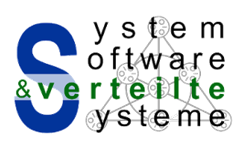
\includegraphics[scale=0.6]{ressourcen/logo_svs.png}
	\end{minipage}
	\begin{minipage}{0.4\textwidth}
		
\includegraphics[scale=0.6]{ressourcen/logo_st.png}
	\end{minipage}
\end{figure}

\end{center}
\end{titlepage}

\ofoot{\pagemark}

% Seitenzahlen vor dem Hauptteil in Römischen Nummern
\pagenumbering{Roman}
\cleardoublepage
% Phantomabsatz, damit die Seitenzahl im Pdf-Betrachter stimmt. (Wird von hyperref benötigt)
\phantomsection
% Einfügen vom Inhaltsverzeichnis ins Inhaltsverzeichnis vorm Generieren des Inhaltsverzeichnis, damit die Seitenzahl stimmt
\addcontentsline{toc}{chapter}{Inhaltsverzeichnis}
\tableofcontents % Inhaltsverzeichnis
\listoffigures % Abbildungsverzeichnis
\listoftables % Tabellenverzeichnis
\setcounter{counterListPage}{\value{page}}
\addtocounter{counterListPage}{1}
\clearpage

% Seitenanker wieder aktivieren
\hypersetup{pageanchor=true}
% Seitenzahlen für den Hauptteil in Arabischen Nummern
\pagenumbering{arabic}
% Das eigentliche Dokument (Hauptteil)

\chapter{Projekthandbuch}

\section{Rollen und Besetzungen}
Die Rollen und ihre Besetzung haben sich über das Projekt teilweise verändert, da wir nach der Anforderungsanalyse agil mit Scrum gearbeitet haben. Deswegen wird im folgenden zu erst auf die initialen Rollenverteilung eingegangen und anschließend die neue Verteilung beschrieben.

\subsection{Planungsphase}
\subsubsection{Projektleiter} 
\textbf{Besetzung:} Maik Appeldorn \\
Die Rolle des Projektleiters ist in unserem Projekt nicht gleichzusetzen mit der eines herkömmlichen Projektleiters, da viele Aufgaben durch die gesamte PG abgefangen werden.
Die Aufgaben des Projektleiters sind:
\begin{itemize}
	\item Er ist der Kommunikationsknoten zwischen der PG und allen daran Beteiligten
	\begin{itemize}
		\item Er verschickt die Einladungen für die Betreuertreffen und andere Treffen, bei denen externe Personen eingeladen werden. (Externe Personen sind diese, die nicht Mitglied der PG sind, also auch Betreuer)
		\item Er übernimmt außerdem die Kommunikation zu den Projektpartnern/Betreuern und ist die konzentrierte Anlaufstelle
	\end{itemize}	
	\item Er ist in jeder Projektphase grob darüber informiert, mit welchen Aufgaben sich die einzelnen Gruppen gerade beschäftigen, sodass er bei Bedarf zwischen diesen vermitteln kann
	\item Er übernimmt die Kontrolle des Projektfortschritts (Zeit/ Kosten/ Arbeitsfortschritt)
\end{itemize}

\subsubsection{Stellvertretender Projektleiter}
\textbf{Besetzung:} Dennis Rupprecht \\
\begin{itemize}
	\item Der stellvertretende Projektleiter bleibt in stetigem Kontakt mit dem Projektleiter und übernimmt dessen Aufgaben z.B. bei Abwesenheit von eben diesem.
	\item Welche Aufgaben damit genau in seinem Verantwortungsbereich liegen: siehe 1.1. Projektleiter
\end{itemize}

\subsubsection{Tools}
\textbf{Besetzung:} Dennis Rupprecht \\
\begin{itemize}
	\item Die Vertreter der Rolle \dq Tools\dq  ist dafür zuständig, dass der Atlassian-Stack richtig konfiguriert wird.
	\item Bei Fragen zu Tools ist er in der Verantwortung, die Fragen zu beantworten, ggf. mit Hilfe von Recherche.
\end{itemize}

\subsubsection{Qualitätsmanagement}
\textbf{Besetzung:} Tamme Janßen, Sona Hayrapetyan, Christian Linder \\
Die Qualitätsmanager haben diverse Aufgaben, um die Qualität des Produkts und der Prozesse zu gewährleisten:
\begin{itemize}
	\item Überprüfung der Jira-Tickets auf korrekte Formulierung und Pflege der Tickets
	\begin{itemize}
		\item Priorität, Ticketbeschreibung, Name, Bearbeiter, Aufwandsschätzung (optional), Tatsächliche Dauer (Tempo-Plugin) etc.
		\item Ticketnummer zur Referenz in der Commit-Beschreibung
	\end{itemize}
	\item Sicherstellung der Qualität durch Tests (muss noch näher beschrieben werden)
	\begin{itemize}
		\item Mocking (Abhängigkeiten) / JUnit - Testprojekt für jedes Modul
	\end{itemize}
	\item Definition of Done für User Stories - Fertigstellungskritierien eines Pull-Request's
	\item Festlegung der Workflows von Jira-Tickets
	\item Sicherstellung der Usability
	\begin{itemize}
		\item Einführung eines Style-Guides (Vorgaben) in Confluence (Vorgaben über die Usability)
		\item Spätere Evualation an Kommilitonen (Umfrage über die Usablity beim Zwischenergebnisse)
	\end{itemize}
	\item Einführung von Code-Conventions in Form einer Konfiguration (Wie der Code-Style zwischen den Entwicklern aussieht.)
	\begin{itemize}
		\item Dazu kann z. B. in Intellij das Plugin Checkstyle verwendet werden.
	\end{itemize}
	\item Logging mit Hilfe von Log4j2 (optional)
	\item Fortschritt und Qualität der Dokumentation sicherstellen
	\item Kontrolle der Dokumente, die an Personen außerhalb der Projektgruppe herausgegeben werden
	\item Fortlaufende Weiterführung des Projekthandbuches über die gesamte Projektdauer
\end{itemize}

\subsubsection{Moderator}
\textbf{Besetzung:} Maik Appeldorn \\
\begin{itemize}
	\item Der Moderator verliest ggf. das Protokoll der letzten Sitzung
	\item Der Moderator leitet die Sitzung und ist befugt, Regeln während einer Sitzung einzuführen, z.B. Wortmeldungen zur Kommunikation
	\item Der Moderator ist befugt ein "`time boxing"' einzuführen
\end{itemize}

\subsubsection{Protokollant}
\textbf{Besetzung:} wechselnd \\
\begin{itemize}
	\item Der Protokollant verfasst eine Mitschrift der Sitzungen nach einem vorgegebenem Formular
	\item Das Protokoll muss bis zu einem festgelegtem Datum fertig sein, damit es der Projektleiter an die Einladungen anhängen kann
	\item Der Protokollant erstellt im Confluence eine Seite für die Besprechungsnotizen nach einer bestimmte Vorlage
\end{itemize}

\subsubsection{Infrastruktur}
\textbf{Besetzung:} Marcell Stosun \\
\textbf{Stellvertreter:} offen \\
Unter die Rolle des Infrastruktur-Beauftragten fallen:
\begin{itemize}
	\item Die Organisation benötigter Server
	\item Die Administration der Server
	\item Die Sicherstellung der Erreichbarkeit der Server
	\item Das Deployment
\end{itemize}

\subsubsection{Hardwareverwalter}
\textbf{Besetzung:} Jan Johannes Haskamp \\
\textbf{Stellvertreter:} offen \\
Zu den Zuständigkeiten des Hardwareverwalters fallen alle Aufgaben rund um die Sensoren:
\begin{itemize}
	\item Bestandsübersicht über die Sensoren
	\item Verwaltung und Zugriff der Sensoren
	\item Experte im Umgang mit den Sensoren 
	\begin{itemize}
		\item Aufbau, Funktionalitäten
	\end{itemize}
	\item Übersicht über das Sensor-Netzwerk
	\begin{itemize}
		\item Wo besteht Wartungsbedarf?
	\end{itemize}
	
\end{itemize}

\subsubsection{Kassen-Manager}
\textbf{Besetzung:} Jan Brunnberg \\
\begin{itemize}
	\item Der Kassen-Manager ist Verantwortlich für die Verwaltung von Geldern, die bspw. bei Strafen eingenommen werden
	\item Eventuell Eröffnung eines Kontos zur Verwaltung von Einnahmen, wie Strafgeldern oder Projektzuschüssen
	\item Liste mit offenen Strafen pflegen?
\end{itemize}

\subsubsection{Kassen-Prüfer}
\textbf{Besetzung:} Gerrit Schöne \\
\begin{itemize}
	\item Zusätzliche Instanz zum Prüfen der Kasse/Gelder
\end{itemize}

\subsubsection{Teambuilding Beauftragter}
\textbf{Besetzung:} Sona Hayrapetyan \\
\begin{itemize}
	\item Der Teambuilding-Beauftrage sorgt dafür, dass das Team sich auch privat trifft und die Team-Chemie verbessert wird
	\item Es werden mögliche Termine vorgeschlagen und in der Gruppe beschlossen 
\end{itemize}

\subsubsection{Team-Verantwortliche}
\begin{itemize}
	\item In jedem Team, das eine spezielle Aufgaben, bzw. einen Teilbereich des Projektes übernimmt, wird ein Teamleiter bestimmt
	\item Der Teamleiter informiert den Projektleiter über den Fortschritt und die Aufgaben des Teams
\end{itemize}

\subsection{Implementierungsphase}
In der Implementierungsphase wird auf agiles Arbeiten umgestellt, wodurch sich neue Rollen ergeben haben bzw. alte Rollen angepasst oder neu besetzt werden. Beispielsweise wird die Rolle des Projektleiters verändert in die Rolle des Scrum Masters.

\subsubsection{Scrum Master}
\textbf{Besetzung:} Maik Appeldorn, Gerrit Schöne \\
\begin{itemize}
	\item Der Scrum Master ersetzt den Projektleiter und den Moderator und übernimmt somit deren Aufgaben.
	\item Er trägt Verantwortung für den Scrum-Prozess und dessen korrekte Implementation.
	\item Er ist ein Vermittler und Unterstützer.
	\item Er sorgt für Informationsfluss zwischen Product Owner und Team.
	\item Er moderiert Scrum-Meetings.
	\item Er hat die Aktualität der Scrum-Artefakte (Product Backlog, Sprint Backlog, Burndown Charts) im Blick.
	\item Er schützt das Team vor unberechtigten Eingriffen während des Sprints.
\end{itemize}
\subsubsection{Product Owner}
\textbf{Besetzung:} Jan Brunnberg, Jacqueline Klimmek, Tamme Janßen \\
\begin{itemize}
	\item Pflege des Product Backlogs.
	\item Priorisiert die Product Backlog Items so, dass es dem Projektplan entspricht.
	\item Steht für Rückfragen des Teams bereit
	\item Vorbereitung und Leitung der Refinement Termine
\end{itemize}
\subsubsection{Qualitätsmanager}
\textbf{Besetzung:} Muhammad Ekbal Ahmad \\
\begin{itemize}
	\item Neubesetzung der Rolle, Aufgaben bleiben gleich 
\end{itemize}
\subsubsection{Datenanalyst}
\textbf{Besetzung:}  Sona Hayrapetyan, Dennis Rupprecht, Marcell Stosun \\
\begin{itemize}
	\item Analysiert die gemessenen Daten der Sensorknoten auf Auffälligkeiten und Ausreißern. 
	\item z.B. Verlässlichkeit der Sensoren, Bereich in dem sich die Feinstaubwerte verändern, ...
\end{itemize}

\subsubsection{Sensorknotenbeauftragter}
\textbf{Besetzung:}  Christian Linder, Jan Johannes Haskamp\\
\begin{itemize}
	\item Verwaltung der Hardware
	\item Planung der Sensorknotenabdeckung.
	\item Ausbringung von Sensorknoten.
\end{itemize}

\section{Projektbeteiligte}
\subsection{Projektgruppenmitglieder}
\begin{table}[!ht]
	\centering
	\begin{tabular}{|c|c|c|c|}
		\hline
		\textbf{Name} & \textbf{E-Mail} \\ \hline
		Muhammad Ekbal Ahmad & \mailaddr{muhammad.ekbal.ahmad@uni-oldenburg.de} \\ \hline
		Maik Appeldorn & \mailaddr{maik.appeldorn@uni-oldenburg.de} \\ \hline
		Jan Brunnberg & \mailaddr{jan.brunnberg@uni-oldenburg.de} \\ \hline
		Jan Johannes Haskamp & \mailaddr{jan.johannes.haskamp@uni-oldenburg.de} \\ \hline
		Sona Hayrapetyan & \mailaddr{sona.hayrapetyan@uni-oldenburg.de} \\ \hline
		Tamme Janßen & \mailaddr{tamme.janssen@uni-oldenburg.de} \\ \hline
		Jacqueline Klimmek & \mailaddr{jacqueline.klimmek@uni-oldenburg.de} \\ \hline
		Christian Linder & \mailaddr{christian.linder1@uni-oldenburg.de} \\ \hline
		Dennis Rupprecht & \mailaddr{dennis.rupprecht@uni-oldenburg.de} \\ \hline
		Gerrit Schöne & \mailaddr{gerrit.schoene@uni-oldenburg.de} \\ \hline
		Marcell Stosun & \mailaddr{marcell.stosun@uni-oldenburg.de} \\ \hline
	\end{tabular}
\end{table}
\FloatBarrier

\subsection{Abteilung Softwaretechnik}
\paragraph{Andreas Winter} Betreuer \\
\textbf{E-Mail}: \mailaddr{winter@se.uni-oldenburg.de}

\paragraph{Dilshodbek Kuryazov} Betreuer \\
\textbf{E-Mail}: \mailaddr{kuryazov@se.uni-oldenburg.de}

\paragraph{Ruthbetha Kateule } Betreuer \\
\textbf{E-Mail}: \mailaddr{ruthbetha@se.uni-oldenburg.de}

\subsection{Abteilung verteilte Systeme}
\paragraph{Oliver Theel} Betreuer \\
\textbf{E-Mail}: \mailaddr{theel@informatik.uni-oldenburg.de}

\subsection{embeteco}
\paragraph{Oliver Norkus} Projektpartner \\
\textbf{E-Mail}: \mailaddr{on@embeteco.de}

\subsection{BTC}
\paragraph{Christian Hinrichs} Projektpartner \\
\textbf{E-Mail}: \mailaddr{christian.hinrichs@btc-ag.com}

\paragraph{Michael Stadler} Projektpartner \\
\textbf{E-Mail}: \mailaddr{michael.stadler@btc-ag.com}

\section{Kommunikation}
\subsection{Interne Kommunikation}
Die interne Kommunikation der Projektgruppe findet über 2 Kommunikationskanäle statt:
\begin{itemize}
	\item Slack
	\item Confluence
\end{itemize}

\paragraph{Slack} Über Slack können Privat- und Gruppen-nachrichten ausgetauscht werden. Diese Kommunikations Ebene ist von unformeller Natur und dient ausschließlich zum schnellen Austausch von Informationen und Fragen.

\paragraph{Confluence} Confluence dient zur Archivierung der internen Kommunikation und in diesen stattfindenden Entscheidungen. Dies betrifft zum Beispiel einen Kalender, in welchen Urlaubstermine und Arbeitstermine eingetragen werden, aber auch Sitzungs- und Entscheidungsprotokolle. 

\subsection{Kommunikation mit den Betreuern/Projektpartnern}
Bei der Kommunikation mit den Betreuern und anderen Projektpartnern wird ausschließlich die E-Mail verwendet. In diesen werden unter anderen Dokumente (immer als PDF), sowie Einladungen (mit Agenda und Ziel) verschickt. Die Kommunikation läuft ausschließlich über den Projektleiter. \\
\textbf{Mail-Verteiler:} \mailaddr{pg-rio@informatik.uni-oldenburg.de} (Enthält alle Projektgruppenmitglieder und -betreuer)

\subsection{Kommunikation mit externen Personen}
Die Kommunikation zu außen stehenden Personen erfolgt über den Projektleiter, um möglichen Verwirrungen vorzubeugen. In Einzelfällen kann die Kommunikation von einer im entsprechenden Thema involvierten Person erfolgen. Dann ist der Projektleiter beim Versenden externer Mails in cc: zu nehmen.\\
\textbf{Mail-Verteiler:} \mailaddr{pg-rio-alle@informatik.uni-oldenburg.de} (Enthält alle Projektgruppenmitglieder, -betreuer und externen Partner)

\section{Sitzungsablauf}
\subsection{Betreuertreffen}
Das Treffen mit den Betreuern am Dienstag von 10 bis 12 Uhr folgt immer den gleichen Ablauf:
\begin{enumerate}
	\item Weekly Scrum ~15 Minuten
	\item Termin-spezifische Agenda ~45 Minuten - 1 Stunde
	\item Nachbereitung des Feedbacks ~45 Minuten - 1 Stunde
\end{enumerate}

\subsection{Sprint Meeting}
Am Ende eines jedes Sprintes findet am Montag ein Sprint Meeting statt, in welchen der Sprint durch Reviews abgeschlossen und der neue Sprint im Form eines Sprint Plannings gestartet wird.

Der genaue Ablauf eines Sprint Meetings sieht wie folgt aus:
\begin{enumerate}
	\item Sprint Review ~30 Minuten
	\item Sprint Retrospektive ~30 Minuten
	\item Backlog Refinement ~30 Minunten
	\item Pause
	\item Sprint Planning ~1 Stunde
\end{enumerate}

\subsection{Arbeitstermin}
Der Arbeitstermin, welcher Montags von 10 bis 14 Uhr stattfindet folgt ebenfalls einen immer festen Schema:
\begin{enumerate}
	\item Agenda ~ 30 Minuten
	\item Diskussionspunkte ~15 - 20 Minuten (Pro Punkt maximal 2-3 Minunten)
	\item Aufgabenverteilung ~ 15 - 30 Minuten
	\item Pause
	\item Arbeit in den Kleingruppen
\end{enumerate}

\section{Regeln}
\subsection{Urlaub}
Bei längerfristigen Abwesenheiten (>5 Tage) sollte möglichst frühzeitig (mind. 2-3 Wochen vorher) Bescheid gegeben werden, inwiefern man in dieser Zeit mitarbeiten kann und wann genau der Aufenthalt ist. Dies ist ebenfalls in Confluence-Kalender einzutragen.

\subsection{Überprüfen der E-Mails}
Während des Projektes läuft ein Großteil der Kommunikation mit den Betreuern und weiteren Stakeholdern über Email. Zudem werden die Einladungen zu wichtigen Treffen in Form von Mails verschickt.
\begin{itemize}
	\item Jedes Projektmitglied sollte mindestens einmal am Tag in seine Mails gucken	
\end{itemize}

\subsection{Unentschuldigtes zu spät kommen}
Termine starten immer um Punkt (XX:\textbf{00}), falls es keine andere Information dazu gab. Kommt man zu spät ohne dies vorher anzumerken so existieren gestaffelte Strafen: \\
Alle \textbf{angebrochenen} 5 Minuten resultieren in 2\euro{} Strafe mit einem Maximum von 30\euro{}.



\newcommand{\textbi}[1]{\textit{\textbf{#1}}}

\section{Verwaltung von Artefakten}
\subsection{Aufgaben}
Die anstehenden, laufenden und fertiggestellten Aufgaben der Projektgruppe werden im PGRIO-Projekt des JIRA-Servers gepflegt. (\url{https://jira.swl.informatik.uni-oldenburg.de}) Zugang haben alle Projektgruppenmitglieder. Die Verwaltung der Zugänge wird von der Rolle Atlassian übernommen, in Kommunikation mit Marco Grawunder. (\mailaddr{marco.grawunder@uol.de})

\paragraph{Aufgabenboard}
In der Anfangsphase des Projekts (Definitionsphase) wird das Aufgabenboard verwendet. Darin werden Tickets vom Typ Task erfasst und um Sub-Tasks ergänzt, um die Bearbeitung der anstehenden Aufgaben zu organisieren. Im Aufgabenboard gibt es die Spalten "`To Do"', "`In Progress"', "`In Review"', "`Done"'. Der Workflow ist unter Entwicklungsworkflow erklärt.

\paragraph{Weitere Boards}
Mit Beginn der Anforderungsanalyse wird ein weiteres Board zur Organisation der Anforderungen innerhalb des Backlogs verwendet. Dieses ist noch zu erstellen und zu erläutern.

\subsection{Dokumentation}
\paragraph{Source Code Dokumentation}
Der Source Code der einzelnen Teilprojekte ist jeweils zu dokumentieren. Hier werden die Richtlinien festgehalten, welche Code-Bestandteile wie zu dokumentieren sind. Beschreibung der Richtlinien folgt spätestens vor Beginn der Entwicklungsphase.

\paragraph{Weitere Dokumentation}
Weitere Dokumentation ist soweit möglich in Confluence zu pflegen. Die Dokumentation muss folgende Bestandteile beinhalten:
\begin{itemize}
	\item Benutzerdokumentation
	\begin{itemize}
		\item Installation und Hilfe zur Routinganwendung
		\item Einrichtung, Inbetriebnahme und Wartung von Sensoren
	\end{itemize}
	\item Testdokumentation
	\begin{itemize}
		\item Definition Testfälle
		\item Durchführung von Tests
	\end{itemize}
	\item Infrastruktur/ Deployment
	\begin{itemize}
		\item Beschreibung der Systeminfrastruktur (Testumgebung/ Produktivumgebung)
		\item Anleitung zur Durchführung eines Deployments
		\item Beschreibung automatischer Deployment-Verfahren
	\end{itemize}
	\item Schnittstellenbeschreibung
	\begin{itemize}
		\item Protokolle
		\item Endpunkte
	\end{itemize}
	\item Methodendokumentation
	\begin{itemize}
		\item z.B. Beschreibung verwendeter Algorithmen
	\end{itemize}
\end{itemize}

\subsection{Source Code}
\paragraph{Überblick}
Der Source Code des Projekts wird in der Bitbucket Quellcode-Verwaltung abgelegt. (\url{https://git.swl.informatik.uni-oldenburg.de/projects/PGRIO}) Durch die Verwendung der Quellcode-Verwaltung mit Git wird die gemeinsame Arbeit am Code erleichtert und sicherer gestaltet.\\
Der Source Code teilt sich auf verschiedene Teilprojekte auf, die im Folgenden erläutert und ggf. ergänzt werden.

\paragraph{Wie lege ich ein Teilprojekt an?}
Zum Anlegen eines Teilprojektes gehören folgende Schritte:
\begin{itemize}
	\item Anlegen des Git-Repositories im PGRIO-Projekt
	\item Bestimmung eines Teilprojekt-Verantwortlichen und ggf. eines Stellvertreters
	\item Festlegen der verwendeten Technologien
	\begin{itemize}
		\item Programmiersprache
		\item Frameworks
		\item Entwicklungstools und -umgebung
	\end{itemize}	
	\item Festlegen der Branching-Strategie
	\item Festlegen der Code-, Test- und Dokumentationsrichtlinien für das Teilprojekt
	\begin{itemize}
		\item Standard-Konventionen der verwendeten Technologie bevorzugen
	\end{itemize}
	\item Ggf. Festlegen besonderer Qualitätssicherungsmaßnahmen
	\item Initialen Commit und ggf. initiales branchen vornehmen (Erste Projektstruktur)
	\item CI/CD einrichten
	\item Dokumentation des Teilprojektes im Projekthandbuch
	\begin{itemize}
		\item Name
		\item Verantwortlicher (und Stellvertreter)
		\item Verwendete Technologien (mit kurzer Begründung)
		\item Branch-Strategie
		\item Code-Richtlinien
		\item Test-Richtlinien
		\item Dokumentations-Richtlinien
		\item Erläuterung zum CI/CD
		\item Qualitätssicherungsmaßnahmen
	\end{itemize}	
	\item Feedback zu diesem Kapitel des Projekthandbuchs
\end{itemize}

\paragraph{Wie beginne ich die Arbeit am Source Code?}
Zum Beginnen der Arbeit an einem Teilprojekt sind folgende Schritte notwendig:
\begin{itemize}
	\item Rücksprache mit Verantwortlichem
	\item Einrichtung der Entwicklungsumgebung
	\item Pull des Quellcodes
	\item Einlesen in Branching-Strategie, Code- und Dokumentationsrichtlinien sowie Qualitätssicherungsmaßnahmen
	\item Einarbeitung in den Code
	\item Rückfragen stellen
	\item Gemeinsam loslegen
\end{itemize}

\paragraph{Wie wird die Codequalität gesichert?}
Der Code wird durch den Entwicklungsworkflow (Pull-Requests), durch gemeinsame Code Reviews und durch automatische Tests gesichert, die durch Pipelines automatisch nach einem Push ausgeführt werden. Beim Review eines Merge-Requests und bei Durchführung eines gemeinsamen Code Reviews sind die Einhaltung der Code-, Test- und Dokumentationsrichtlinien zu überprüfen. Zudem werden die Implementation und automatische Tests gegenüber der Spezifikation der umgesetzten Aufgabe überprüft. Zu den einzelnen Teilprojekten können weitere Qualitätssicherungsmaßnahmen festgelegt werden.

\paragraph{Teilprojekte}
Hier werden die einzelnen Teilprojekte, wie oben beschrieben, dokumentiert.

\begin{enumerate}
	\item dokumentation
	\begin{itemize}
		\item Verantwortlich: Gerrit Schöne
		\item Technologien: Latex
		\item Branch-Strategie: Jeder Task/Subtask wird in einem eigenen Branch bearbeitet.
		\item Qualitätssicherung: Änderungen werden über einen Pull-Request in den master Branch eingespielt. Der Pull-Request ist von einer anderen Person zu überprüfen, kleine Anpassungen wie Rechstschreibkorrektur dürfen vom Prüfer vorgenommen werden. Danach kann der Pull-Request akzeptiert oder mit Anmerkungen abgewiesen werden.
	\end{itemize}
\end{enumerate}

\subsection{Modelle}
Folgende Modelle der Software werden in Confluence hinterlegt und sind stets aktuell zu halten:
\begin{itemize}
	\item Systementwurf
	\item Softwarearchitektur
\end{itemize}

\subsection{Sitzungsprotokolle}
\paragraph{Überblick}
Zu allen Besprechungsterminen wird ein Sitzungsprotokoll angefertigt und im Confluence abgelegt. Dafür gibt es die Oberseite Sitzungen, unter der die Protokolle abgelegt werden. Die Namenskonvention zum Abspeichern ist „YYYY-MM-DD \{Art der Besprechung\}“.

\paragraph{Welche Arten von Sitzungen gibt es?}
\begin{itemize}
	\item Teamsitzung
	\item Betreuertreffen
	\item \textit{Backlog Refinement}
	\item \textit{Sprint Planning}
	\item \textit{Sprint Review}
	\item \textit{Sprint Retrospektive}
	\item \textit{Code Review}
\end{itemize}
Die kursiv dargestellten Sitzungen sind derzeit noch nicht beschrieben.

\paragraph{Wer schreibt das Protokoll?}
Die Protokolle werden reihum von verschiedenen Teammitgliedern geschrieben. Der Protokollant wird wochenweise für alle Sitzungen der Woche festgelegt. Wer in welcher Woche Protokollant ist, wird in einer Übersicht auf der Oberseite Sitzungen festgehalten.

\paragraph{Wie wird das Protokoll vom Protokollanten vorbereitet?}
Der Protokollant legt die Seite im Confluence frühzeitig vor der Besprechung an. Die Agenda wird anhand des letzten Protokolls in Rücksprache mit dem Moderator festgelegt. Zum Anlegen gibt es verschiedene Vorlagen im Confluence. Die Namenskonvention ist zu berücksichtigen und Moderator sowie Protokollant sind in das Protokoll einzutragen. \\
\textbi{Teamsitzung / Betreuertreffen}:
Für diese Besprechungen gibt es die Confluence-Vorlage Besprechungsnotizen. Bei Teamsitzungen findet kein Weekly Scrum statt, dieser Abschnitt kann für diese Besprechungen also entfernt werden.

\paragraph{Wie bereiten sich die Teammitglieder auf Sitzungen vor?}
Allgemein gilt es, sich auf die Themen der Besprechung ausreichend vorzubereiten. Dazu zählt insbesondere das Vorbereiten von Themen, die man selbst vorstellt. Dazu kann auch im Vorfeld ein Dokument an die anderen Teilnehmer versendet werden. Das Durchlesen dieser Dokumente zählt genauso zur Vorbereitung auf die Sitzung.\\
\textbi{Teamsitzung}:
Hier kann jedes Teammitglied im Vorfeld unter Diskussionspunkte Themen mit einbringen, die innerhalb von ca. 5 Minuten besprochen werden können.\\
\textbi{Betreuertreffen}:
Hier ist von jedem Mitglied die Tabelle des Weekly Scrums im Vorfeld auszufüllen.

\paragraph{Wie wird protokolliert?}
Protokolliert werden die Ergebnisse und Entscheidungen der Sitzung. Dazu wird zu jedem Punkt der Agenda eine Übersicht der besprochenen Ergebnisse und der getroffenen Entscheidungen dargestellt. Ergänzend werden bei Diskussionen wichtige Argumente für und gegen eine Variante festgehalten. Bleiben offene Fragen oder Entscheidungen werden vertagt, ist dies ebenfalls zu protokollieren. Abgeleitete Aufgaben aus der Sitzung werden am Ende des Protokolls in einer Übersicht mit Bearbeiter der Aufgabe zusammengefasst.

\paragraph{Wie wird das Protokoll nachgearbeitet?}
Das Protokoll wird vom Protokollanten aufbereitet, um korrekte Rechtschreibung und eine gute Formulierung zu gewährleisten. Zusätzlich soll das Protokoll von einer weiteren Person auf Rechtschreibung und Formulierung geprüft werden. Danach wird das Protokoll freigegeben und als PDF exportiert, damit es mit der nächsten Einladung an die Projektbeteiligten verschickt werden kann. Jedes Projektgruppenmitglied erstellt eigenverantwortlich JIRA-Tickets für seine Aufgaben.

\subsection{Sonstige Artefakte}
Folgende Artefakte werden mittels Latex im Repository dokumentation der Source Code-Verwaltung gepflegt:
\begin{itemize}
	\item Visionsdokument
	\item Projekthandbuch
\end{itemize}
Entstehen im Entwicklungsprozess weitere Artefakte, so ist hier zu dokumentieren, wo und in welcher Form sie zu hinterlegen sind. Bestenfalls werden sonstige Artefakte in Confluence oder in der Quellcode-Verwaltung hinterlegt.


\providecommand{\vmodelFirstSection}[1]{\section{#1}}
\providecommand{\vmodelSecondSection}[1]{\subsection{#1}}
\providecommand{\vmodelThirdSection}[1]{\subsubsection{#1}}

\vmodelFirstSection{Vorgehensmodell}
\begin{figure}[!ht]
	\centering
	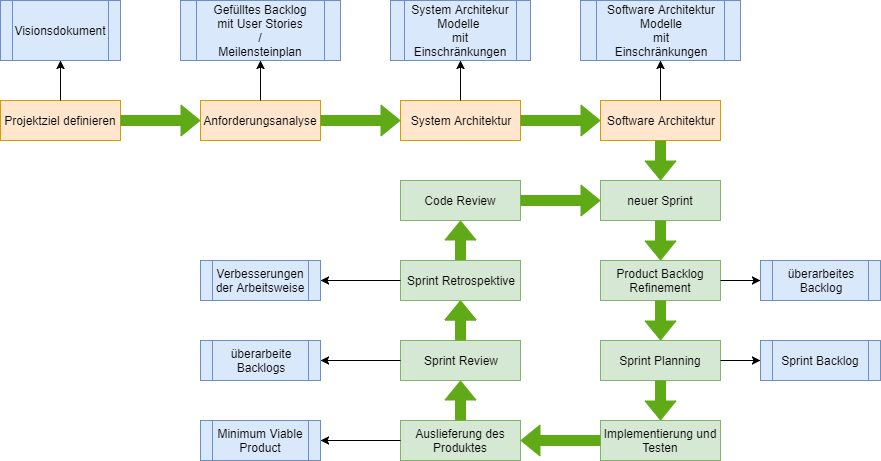
\includegraphics[width=1.0\linewidth]{./ressourcen/vorgehensmodell.png}
	\caption{Vorgehensmodell}
	\label{fig:sec:vorgehensmodell}
\end{figure}
Das Vorgehensmodell der Projektgruppe (siehe \Fig{sec:vorgehensmodell}) besteht aus 2 Abschnitten:
\begin{enumerate}
	\item Wasserfall-ähnliche Definitionsphase
	\item Agile Implementations-und Entwicklungsphase
\end{enumerate}
Die Dokumentation von Entscheidungen und anderen wichtigen Artefakten ist ein fortlaufender Prozess, welcher sich über beide Projektphasen erstreckt.

\vmodelSecondSection{Definitionsphase}
Die am Anfang stattfindende Definitionsphase beinhaltet in chronologischer Reihenfolge folgende Aktivitäten:
\begin{enumerate}
	\item Projektziel definieren
	\item Anforderungsanalyse 
	\item System Architektur definieren
	\item Software Architektur definieren
\end{enumerate}

\vmodelThirdSection{Projektziel definieren}
Während der Aktivität der Projektziel Definition wird ein minimales Projektziel erarbeitet, welches mit allen beteiligten Stakeholdern abgestimmt wurde.
Dieses Projektziel wird in einem \textbf{Visionsdokument} festgehalten, welches ebenfalls eine Einleitung zum Problem enthält und versucht das Projektziel abzugrenzen.

\vmodelThirdSection{Anforderungsanalyse}
Während der Anforderungsanalyse werden die wichtigsten Anforderungen definiert, welche das System umsetzen muss.
Wünsche (Kann-Anforderungen) werden hier ebenfalls notiert, um eine mögliche Erweiterung des Systems zu berücksichtigen.

Bei der Analyse ist jedoch darauf zu achten, dass keine vollständige Erfassung der Anforderungen möglich und erforderlich ist, da während der agilen Entwicklungsphase weitere Anforderungen definiert werden können.
Jedoch ist eine möglichst umfangreiche Analyse zu erreichen, ohne dabei zu viel Zeit verstreichen zu lassen.

Während dieser Analyse wird ein \textbf{Anforderungsdokument} erstellt.
Zudem werden Epics und User Stories definiert, die in einem \textbf{gefüllten Backlog} gepflegt und in das Anforderungsdokument integriert werden.

\vmodelThirdSection{System Architektur definieren}
Hier wird die grundlegende System Architektur definiert.
Diese beschreibt gegebene Schnittstellen und zeigt welche Teil"=Systeme untereinander in welcher Richtung kommunizieren.
Nach dieser Aktivität soll ein Modell erstellt sein, welches die \textbf{Systemarchitektur} darstellt. 

\vmodelThirdSection{Software Architektur definieren}
Während dieser Aktivität werden die Teil"=Systeme genauer definiert und die Schnittstellen ebenfalls.
Nach Beendigung der Aktivität "`Software Architektur definieren"' werden als Artefakte \textbf{Softwarearchitekturen der Teilsysteme} erstellt sein.

\vmodelSecondSection{Entwicklungsphase}
Die Entwicklungsphase wird in mehreren agilen Inkrementen (Sprints) durchgeführt.
Jeder Sprint umfasst die gleichen Aktivitäten in einem typischen Zeitraum von 2-3 Wochen.
\begin{enumerate}
	\item Product Backlog Refinement
	\item Sprint Planning
	\item Implementierung und Testen
	\item Auslieferung des Produktes
	\item Sprint Review
	\item Sprint Retrospektive 
	\item Code Review
\end{enumerate}

\vmodelThirdSection{Product Backlog Refinement}
Während des "`Product Backlog Refinements"' werden besonders die an der Spitze des Backlogs stehenden Epics und User Storys überprüft.
Hier werden insbesondere Schätzungen und Prioritäten überprüft, aber auch Epics werden in kleinere User Storys zerteilt.
Das Refinement des Backlogs hat den Sinn der Reduzierung des Aufwandes während des Sprint Planning, da beim Refinement ebenfalls Abhängigkeiten zwischen verschiedenen User Storys gefunden werden können.

\vmodelThirdSection{Sprint Planning}
Beim Sprint Planning wird entschieden welche User Storys umgesetzt werden.
Zusätzlich wird festgelegt wie die Umsetzung erfolgt und wer sie übernimmt.
Hierfür findet eine Teilung des Sprint Plannings in 2 Phasen statt:
\begin{enumerate}
	\item Festlegung des Was
	\item Festlegung des Wie/Wer
\end{enumerate}

\vmodelThirdSection{Implementierung und Testen}
Während der Implementierung werden die geplanten User Storys und Bugs des Sprints umgesetzt.
Dazu werden in den jeweiligen Teil"=Teams Unteraufgaben erstellt, zu denen ein Zweig im jeweiligen Repositorium angelegt wird.
In diesem werden alle zugehörigen Code"=Änderungen zur Unteraufgabe eingespielt.
Nach Fertigstellung wird ein Pull"=Request in den \textit{develop}"=Branch gestellt, der durch mindestens ein anderes Teammitglied überprüft und genehmigt wird.
Siehe hierzu auch \Fig{sec:vorgehensmodell:branchmodell}.

\begin{figure}[!ht]
	\centering
	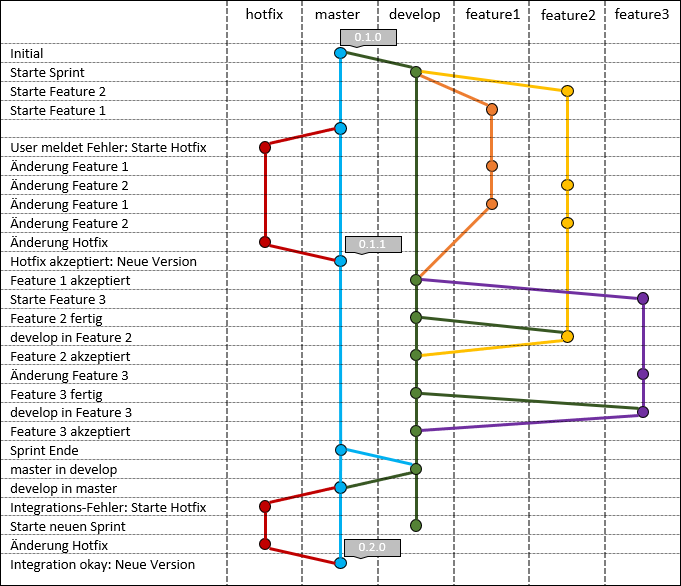
\includegraphics[width=1.0\linewidth]{./ressourcen/Vorgehensmodell_Branchmodell}
	\caption{Branchmodell}
	\label{fig:sec:vorgehensmodell:branchmodell}
\end{figure}

Beim Testen werden einerseits Unit- und Integratiostests im Code geschrieben, die automatisiert ausführbar sind.
Andererseits wird die neue Funktionalität explorativ gegen die Akzeptanzkriterien getestet.
Erst mit bestandenen Tests kann eine User Story abgeschlossen werden.

\vmodelThirdSection{Auslieferung des Produktes}
Nach jedem Sprint Ende wird die erarbeitete Version des Systems "`ausgeliefert"'.
Hierbei wird es sich in der Regel um ein Deployment der überarbeiteten Programme handeln.
Damit im nächsten Sprint mit den Änderungen gearbeitet werden kann.

\vmodelThirdSection{Sprint Review}
Sprint Reviews sind dafür da, um festzustellen, welche User Storys geschafft worden sind und welche noch Arbeit benötigen.
Dieser Schritt hilft, um einen Überblick über den aktuellen Planungs- und Entwicklungsstand zu erhalten.
Darüber hinaus bietet der Review den Steakholdern die Möglichkeit, neue Funktionalitäten vorgestellt zu bekommen und Rückmeldungen sowie Wünsche zu äußern.

\vmodelThirdSection{Sprint Retrospektive}
Während einer Sprint Retrospektive wird die Arbeitsweise während eines Sprints überprüft.
Dafür werden folgende Phasen durchlaufen:
\begin{enumerate}
	\item Informationen sammeln
	\begin{enumerate}
		\item Was lief gut?
		\item Was könnte besser laufen?
	\end{enumerate}
	\item Ursachen herausfinden
	\item Verbesserungsmöglichkeiten bestimmen und anwenden
	\begin{enumerate}
		\item Hier können Aufgaben/Richtlinien entstehen
		\item Änderungen in Projekthandbuch aufnehmen
	\end{enumerate}
\end{enumerate}
Wichtig bei der Retrospektive, aber auch im Allgemeinen ist es ein Arbeitsumfeld zu schaffen, in welchem sich niemand "`schuldig"' fühlt und sich jeder wohl fühlt.

\vmodelThirdSection{Code Review}
Beim Code-Review wird ein Programmabschnitt nach oder während der Entwicklung von einem oder mehreren Gutachtern Korrektur gelesen, um mögliche Fehler, Vereinfachungen oder Testfälle zu finden.
Dabei kann der Gutachter selbst ein Softwareentwickler sein.
Für unerfahrene Entwickler bietet der Code-Review durch einen erfahrenen Programmierer eine gute Möglichkeit, sich schnell und praxisorientiert weiterzubilden.\cite{wiki:codereview}


\section{Wertevorstellung}
Unter Wertevorstellung verstehen wir u.A. Regeln, die jedes Mitglied der Gruppe zum Beispiel beim Gruppengespräch beachten muss. Dazu gehört:
\begin{itemize}
	\item Transparenz gegenüber allen Gruppenmitgliedern, sodass Probleme nicht "`verschluckt"' werden und später wieder aufkommen
	\begin{itemize}
		\item Evtl. zusammen ein Ticket besprechen in den Teams, sodass nicht ein Mitglied alleine aufkommende Probleme behandeln muss
	\end{itemize}
	\item Dem Kommunikationspartner beim Gespräch nicht ins Wort fallen - Ausreden lassen
	\item Keine unnötige Rechtfertigungen
	\begin{itemize}
		\item Kritik annehmen und in der Gruppe die Auswirkungen diskutieren
		\item Keine persönlichen Rechtfertigungen oder Ausreden wie Zeitmangel o.Ä.
		\item Entscheidungen und Abläufe dürfen und sollen aber erklärt werden
	\end{itemize}
	\item Auch über den Tellerrand schauen und nicht nur die eigenen Aufgaben betrachten, sodass z.B. montags nicht alles komplett neu ist
	\item Probleme können offen in den kleinen Gruppen oder um gesamten Team angesprochen werden
	\item Wenn jemand eine Aufgabe erledigt und diese dann im gesamten Team besprochen und kritisiert wird, ist die Kritik nicht persönlich gemeint, sondern sachlich. 
	\begin{itemize}
		\item Kritik muss auch sachlich vorgetragen werden
	\end{itemize}
\end{itemize}

\section{Methoden und Arbeitstechniken}
\subsection{Pair Programming}
Pair Programming (im deutschen Paarprogrammierung) ist eine Methode in der Softwareentwicklung, in welcher die Entwicklung einer Aufgabe von 2 Personen vollzogen wird. Bei der Entwicklung existieren in diesen Paar 2 Rollen:
\begin{enumerate}
	\item Jemand der programmiert
	\item Ein Beobachter, welcher das programmierte überprüft und im Fall eines Problems/Fehlers direkt Feedback gibt
\end{enumerate}
Die Besetzung der Rollen sollte möglichst häufig wechseln. Ein Vorteil dieser Methode ist die Reduzierung von Fehlern, da durchgängig ein Review durch einen anderen Teilnehmer statt findet und hilft somit bei einer schnelleren Fehlerbehebung. Aber auch der Lerneffekt (besonders bei einen Studentenprojekt) ist immens, da neue Techniken direkt an andere Personen weiter getragen wird. Ein weitere wichtiger Punkt neben dem Tausch der Besetzungen bei den Rollen, ist das Durchtauschen der Paare, damit jeder von anderen Teilnehmern des Projektes lernen kann.

\subsection{Planning Poker}
Planning Poker ist eine gamifizierte Methode, um Projektaufgaben ( in unseren Fall User Stories) zu schätzen. Ein wichtiger Punkt beim Planning Poker ist, dass alle Teilnehmer zuerst ihre Schätzung vornehmen bevor man die anderer Teilnehmer sieht. Dadurch schließt man eine Beeinflussung durch andere Schätzungen aus und erhält somit einen besseren Überblick. Ein weiterer wichtiger Punkt ist, dass Schätzungen in so genannten Story Points statt findet und nicht mit Arbeitsstunden, dadurch erhält man ein besseres Gefühl für Komplexität der Aufgabe, aber auch mögliche Ungewissheiten bei einer Aufgabe. Der typischer Ablauf (in unseren Fall) beim Planning Poker ist folgender:
\begin{enumerate}
	\item Moderator (welcher selber keine Schätzung vornimmt) stellt eine zu schätzende Aufgabe/User Story vor
	\item Das Team hat nun die Möglichkeit Fragen zu stellen, um mögliche Unklarheiten aus dem Weg zu räumen
	\item Jedes Mitglied des Teams (außer der Moderator) denkt sich nun eine für ihn plausible Schätzung vor und legt diese Schätzung verdeckt vor sich
	\item Haben alle Mitglieder eine Schätzung vorgenommen werden alle Schätzungen simultan aufgedeckt
	\item Personen mit der höchsten, bzw. niedrigsten Schätzung haben nun die Möglichkeit ihre Schätzung zu erklären
	\item Im Anschluss wird eine weitere Runde geschätzt bis ein Konsens bei dem Team erreicht wurde
\end{enumerate}
Eine wichtige Aufgabe beim Planning Poker kommt den Moderator zu, da dieser die Diskussion leitet und im Auge behält, ob möglicherweise zu viel (unnötige) Zeit beim diskutieren verschwendet wird.

\subsection{Arbeit mit Releases}
Im Rahmen der Entwicklungsphase wird es mehrere größere Releases geben. Diese können sich über mehr als einen Sprint erstrecken. Releases können im Rahmen einer größeren Präsentation vorgestellt werden.
\begin{figure}[!ht]
	\centering
	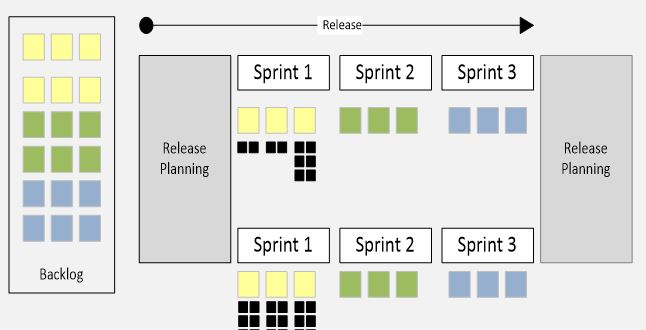
\includegraphics[width=\textwidth]{./ressourcen/release-planning.jpg}
	\caption{Release Planung}
	Source: \url{https://www.scrumdesk.com/wp-content/uploads/Release-planning.jpg}
\end{figure}

\subsection{Entwicklungsworkflow}
\begin{figure}[!ht]
	\centering
	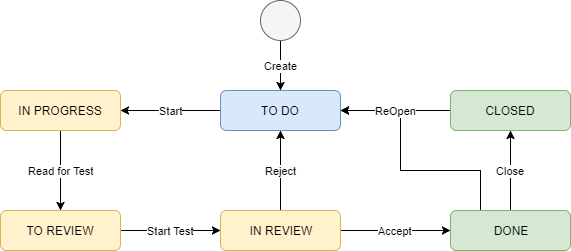
\includegraphics[width=\textwidth]{./ressourcen/entwicklungs-workflow.png}
	\caption{Entwicklungs Workflow}
\end{figure}
Eine Aufgabe/User Story/Epic durchläuft in der Entwicklungsphase immer einen gleichen Workflow. Während diesem Workflow können verschiedene Status erreicht werden:
\begin{description}
	\item[To Do] Aufgabe muss bearbeitet werden
	\item[In Progress] Aufgabe wird derzeitig bearbeitet
	\item[To Review] Aufgabe wurde bearbeitet und kann nun getestet werden
	\item[In Review] Aufgabe wird derzeitig getestet
	\item[Done] Die Aufgabe ist getestet und fertig gestellt
	\item[Closed] Die Aufgabe ist endgültig abgeschlossen (Sprint in welchen die Aufgabe lag ist fertig)
\end{description}
Erstellt man eine Aufgabe wird dieser automatisch der Status "`To Do"' zugewiesen. Aus dem Status "`To Do"' kann nun eine Aufgabe durch starten in den "`In Progress"' Zustand versetzt werden. Ist man nun fertig mit der Implementierung kann man die Aufgabe für das Testen bereit geben in dem man die Aufgabe in "`To Review"' verschiebt. Fängt eine Person an die Aufgabe zu testen verschiebt man diese in "`In Review"', wo man die Aufgabe entweder ablehnen (Status zu "`To Do"' ändern) oder annehmen (Status zu "`Done"' ändern) kann. Sind trotz der Kontrolle noch Fehler in der Aufgabe vorhanden so kann diese von Done/Closed immer wieder in den "`To Do"' Status versetzt werden. Die Transition von "`Done"' zu "`Closed"' erfolgt sobald eine Sprint abgeschlossen ist.


\section{Change Management}
Da ein Hardware/Software Projekt stetigen Änderungen von Anforderungen ausgesetzt ist, folgt in diesen Abschnitt ein Leitfaden zur Bearbeitungen dieser Anforderungsänderungen (Change Requests).
Ein Change Request ist eine Anfrage zu Änderung des Systems und damit in den meisten Fällen eine Anfrage zur Änderung von Anforderungen.
Dieser Änderungswunsch kann mehrere Ursprünge haben, jedoch sind die häufigsten:
\begin{itemize}
	\item Fehler des Systems (Bug)
	\item Erweiterungswunsch eines Nutzers
	\item Event bei der Entwicklung eines anderen Systems
	\item Änderungen in der Struktur oder bei den Standards
\end{itemize}
Tritt einer dieser Punkte auf, so wird im ersten Schritt ein Change Request als Issue in Jira angelegt, welcher durch einen Status gekennzeichnet wird.
In jeder Sitzung wird überprüft, ob Change Requests vorhanden sind.
Sind Change Requests vorhanden, so werden diese auf ihre Möglichkeit in der Umsetzung (Kosten und Nutzen Analyse) geprüft.
Sind Kosten und Nutzen in einen akzeptablen Verhältnis und ist der Change Request in der Projektdauer umsetzbar, so wird dieser Change Request angenommen und in eine normale Anforderung übersetzt, bzw. es werden bestehende Anforderungen angepasst.
Wird der Change Request abgelehnt, so wird dieser derartig gekennzeichnet und mit dem Grund der Ablehnung (als Beschreibung) in Jira archiviert.\label{PHChangeManagement}

\section{Umgang mit JIRA-Tickets}
In diesem Artikel wird beschrieben, welche Funktionen die jeweiligen Tickets im Jira erfüllen und wann diese eingesetzt werden. Man unterscheidet zwischen Epics, User-Stories, Tasks, Sub-Tasks und Bugs.
\begin{figure}[!ht]
	\centering
	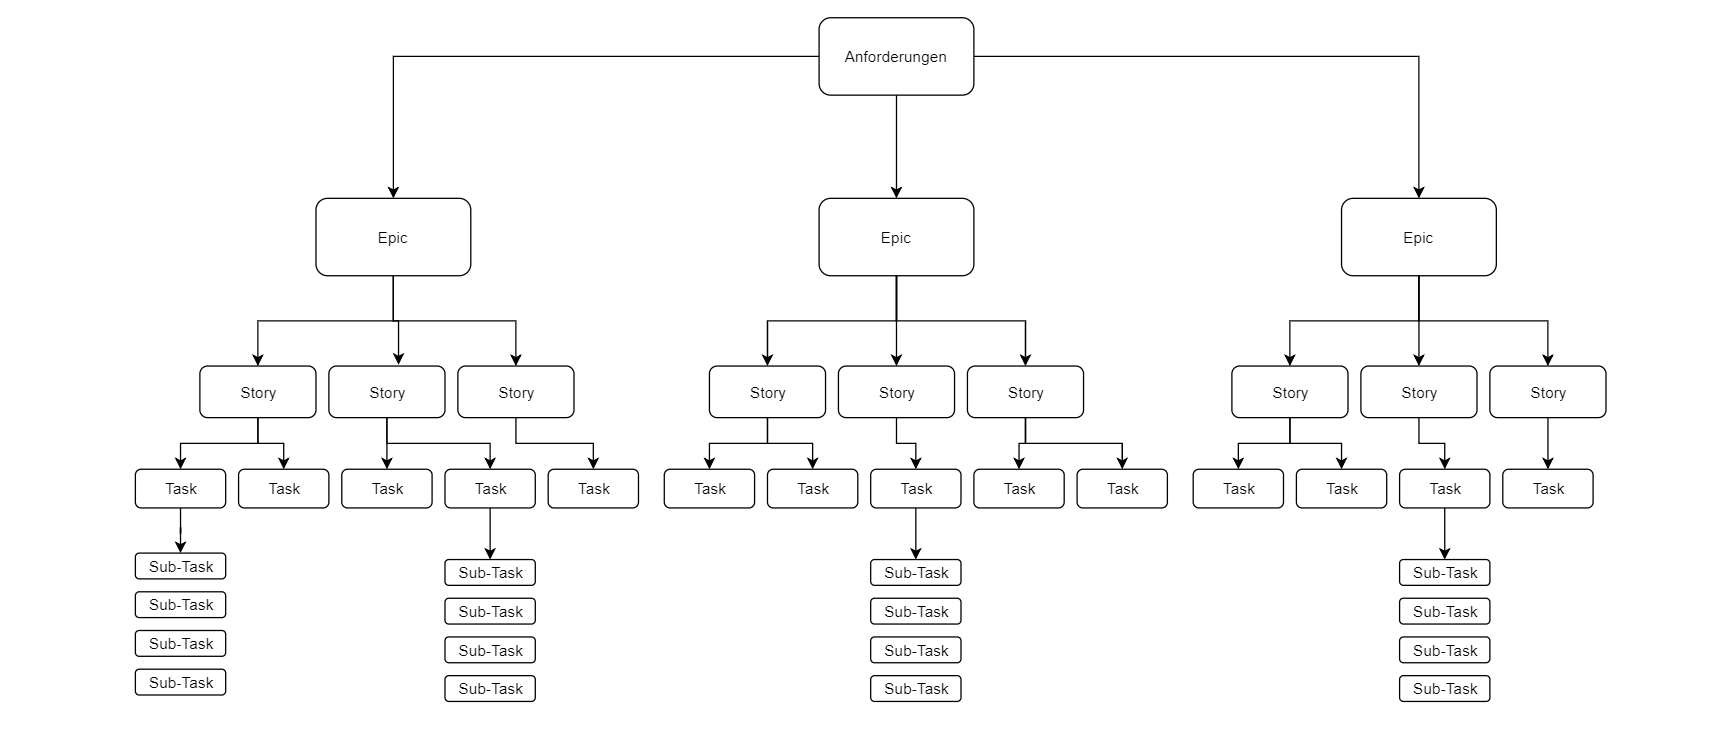
\includegraphics[width=\textwidth]{./ressourcen/jira-hierarchie.png}
	\caption{Hierarchie der "`issue types"' in JIRA}
\end{figure}

\subsection{Epic}
Das Epic das Thema der Umsetzung. Diese wird beispielsweise angelegt, wenn eine neue Funktion in eine Software eingebaut werden soll.\cite{atlassian:jira-support} \\
Ein Epic bildet üblicherweise das Thema einer neuen Umsetzung. Dabei werden die konkreten Anforderungen nicht in einem Epic beschrieben, sondern als zusätzliche Story- oder Task-Tickets formuliert und dann mit dem Epic verlinkt. Das Epic dient also nur der Zusammenfassung aller zugehörigen Anforderungenbei einer größeren Umsetzung von Features oder Ähnlichem.\cite{atlassian:jira-support}

\subsection{User Story}
In einer User-Story werden einzelne Anforderungen aus Sicht des Kunden beschrieben. Die Stories können dann einem Bearbeiter zugewiesen werden, welcher für die Umsetzung der Anforderungen in dem Story-Ticket verantwortlich ist. Zudem können einem Story-Ticket eine "`Defintion of Done"' (DoD), "`Definition of Ready"'  oder andere Kriterien hinzugefügt werden. Anhand der DoD kann der Entwickler zum Beispiel während oder nach der Bearbeitung des Tickets überprüfen, ob er alle ihm zugeordneten Aufgaben erfüllt hat, welche im Zusammenhang mit der Story stehen. Dazu kann zum Beispiel das Erstellen eines Tests gehören oder die korrekte Dokumentation. \cite{scrum-guide}

\subsection{Task}
Bei einer Task werden die User-Stories in weitere Aufgaben zerlegt. Wenn eine Aufgabe eine vereinbarte Zeitspanne überschreitet, kann sie in zusätzliche Aufgaben (Sub-Tasks) aufgeteilt werden. Eine User Story ist dann erledigt, wenn alle beinhaltete Aufgaben erledigt sind. \cite{atlassian:jira-support}



\chapter{Qualitätsmodell}

In diesem Kapitel stellen wir unser Qualitätmodell für die Entwicklung des Gesamtsystems innerhalb des Projekts vor. Dabei betrachten wir die Qualität unserer Software, der verwendeten Daten im System und der unterstützenden Dokumente (Dokumentation, Protokolle). Dabei gehen wir in den einzelnen Bereichen auf verschiedene Qualitätskriterien und Maßnahmen ein, die die Einhaltung der Kriterien überprüfen und sicherstellen sollen. Auf die erweiterte Produktqualität, die auch die verwendete Hardware betrachtet, gehen wir nicht ein, da wir kein Hardwareprodukt entwickeln und vertreiben. Es werden lediglich fertige Bausteine verwendet und Empfehlungen gegeben, wie diese im Zusammenspiel mit unserem System verwendet werden können.

\section{Softwarequalitaet}
Im Folgenden werden die Kriterien für Softwarequalität nach Dimension und Sub"=Dimension tabellarisch aufgezählt. In der Spalte RiO wird dargestellt, ob und wie sehr wir das Kriterium berücksichtigen. In der Spalte Teilsysteme wird aufgelistet, welche Aspekte des Produktivsystems betrachtet werden sollen. In der nächsten Spalte sind die Artefakte und Ressourcen aufgelistet, die zur Sicherstellung der Qualität erstellt und verwendet werden. Unter Maßnahmen werden Vorgehen und Prüfmechanismen zur Sicherung der Qualität bezüglich der betroffenen Dimension aufgelistet.
Zur Nutzbarkeit gibt es einen Sonderfall, da die Unterkriterien für verschiedene Teilkriterien unterschiedlich ausgeprägt sind. Daher wird diese Dimension für jedes betroffene Teilsystem beschrieben.

\begin{landscape}
 \begin{longtable}{|p{4.5cm}|p{1.5cm}|p{4.5cm}|p{4.5cm}|p{3.5cm}|}
 	\caption{Kriterien der Softwarequalität}\\%
   \hline
   Dimension & RiO & Teilsysteme & Artefakte/ Ressourcen & Maßnahmen\\ \hline
   \multicolumn{5}{|c|}{Funktionalität} \\ \hline
   Vollständigkeit & sehr & alle &  Anforderungsdokument & Abnahme Anforderungsdokument, Aufteilung Epics in User Stories\\
   \hline
   Korrektheit & sehr & alle &  Product"=Backlog & User"=Stories, Akzeptanzkriterien, DoD\\ \hline
   Angemessenheit & sehr & alle &  Product"=Backlog & User"=Stories, Akzeptanzkriterien, DoD\\ \hline
   \multicolumn{5}{|c|}{Performance}  \\ \hline
   Zeitliches Verhalten & sehr & Routenberechnung und -bereitstellung, Sensordaten"=Verarbeitung, Services &  Testumgebung, CI/CD"=Server & Performancetests\\ \hline
   Ressourcennutzung & - & - & - & - \\ \hline
   Kapazitäten & - & - & - & - \\ \hline   
   \multicolumn{5}{|c|}{Kompatibilität}  \\ \hline
   Co"=Existenz & - & - & - & - \\ \hline
   Interoperabilität & sehr & IoT"=Plattform & Testumgebung & Integration luftdaten.info \\ \hline
   Dimension & RiO & Teilsysteme & Artefakte/ Ressourcen & Maßnahmen\\ \hline
   \multicolumn{5}{|c|}{Nutzbarkeit (Navigationsanwendung)} \\ \hline
   Angemessene Erkennbarkeit & - & - & - & - \\ \hline
   Lernbarkeit & wenig & - & Testprotokolle & Usertests \\ \hline
   Operabilität & sehr & - & Testprotokolle, Product Backlog & Usertests \\ \hline
   Ästhetik der Nutzeroberfläche & sehr & - & Testprotokolle, Product Backlog & Usertests, Review \\ \hline
   Schutz vor Fehlern & - & - & - & - \\ \hline
   Zugänglichkeit & - & - & - & - \\ \hline  
   \multicolumn{5}{|c|}{Nutzbarkeit (UIS - Anwendung)} \\ \hline
   Angemessene Erkennbarkeit & - & - & - & - \\ \hline
   Lernbarkeit & - & - & - & - \\ \hline
   Operabilität & sehr & - &  & Usertests, Review \\ \hline
   Ästhetik der Nutzeroberfläche & wenig & - & - & Review \\ \hline
   Schutz vor Fehlern & - & - & - & Usertests \\ \hline
   Zugänglichkeit & - & - & - & - \\ \hline   
   Dimension & RiO & Teilsysteme & Artefakte/ Ressourcen & Maßnahmen\\ \hline   
   \multicolumn{5}{|c|}{Wartbarkeit} \\ \hline
   Modularität & sehr & - & Architekturdokument, Source Code & Entwurf Architektur, TDD, Code"=Konventionen \\ \hline 
   Wiederverwendbarkeit & wenig & - & Architekturdokument & Entwurf Architektur \\ \hline    
   Analysierbarkeit & sehr & - & Architekturdokument, IDE, CI/CD"=Server & Entwurf Architektur, TDD \\ \hline
   Modifizierbarkeit & sehr & - & Source Code, CI/CD"=Server & Git, TDD \\ \hline  
   Testbarkeit & sehr & - & Source Code, CI/CD"=Server, Testprotokolle & Akzeptanztests, TDD, DoD \\ \hline   
   \multicolumn{5}{|c|}{Portabilität} \\ \hline    
   Installierbarkeit & sehr & Sensorknoten, Navigations"=App & Testprotokolle & Usertests \\ \hline
   Austauschbarkeit & sehr & IoT"=Plattform & Testumgebung & Integration luftdaten.info \\ \hline   
   Anpassungsfähigkeit & wenig & Sensorknoten & Testumgebung & Integration luftdaten.info \\ \hline 
   \multicolumn{5}{|c|}{Zuverlässigkeit} \\ \hline
   Reife & - & - & - & - \\ \hline
   Fehlertoleranz & - & - & - & - \\ \hline
   Wiederherstellbarkeit & - & - & - & - \\ \hline
   Verfügbarkeit & sehr & Routing, Navigation & - & Log"=Analyse, Benachrichtigungen \\ \hline
   \multicolumn{5}{|c|}{Sicherheit} \\ \hline
   Unwiderruflichkeit & - & - & - & - \\ \hline   
   Vertraulichkeit & sehr & IoT"=Plattform & - & Rollen- und Rechtemanagement \\ \hline 
   Integrität & sehr & IoT"=Plattform & - & Rollen- und Rechtemanagement \\ \hline 
 \end{longtable}
\end{landscape}

\begin{itemize}
    \item	\textit{Anforderungsdokument}: Hier werden die Anforderungen an das System aus Nutzersicht in Form von Epics dargestellt.
    \item	\textit{Product"=Backlog}: Im Product"=Backlog werden die User"=Storys beschrieben und priorisiert, die die Anforderungen der Epics detaillierter beschreiben. Das Backlog wird mittels JIRA gepflegt.
    \item	\textit{Testumgebung}: Die Testumgebung ist eine Spiegelung des sich im produktiven Einsatz befindenden Gesamtsystems. In ihr können neue Funktionalitäten und Anwendungsfälle getestet und überprüft werden. Auf sie kann nur von Projektgruppenmitgliedern zugegriffen werden und sie ist vom Produktivsystem strikt getrennt.
    \item	\textit{CI/CD"=Server}: Dieser Server ermöglicht eine automatische Erstellung der Programme/Komponenten des Systems auf Grundlage des Source"=Codes. Darüber hinaus lassen sich die erstellten Artefakte in der Testumgebung bzw. im Produktivsystem bereitstellen.
    \item	\textit{Testprotokolle}: Zur Beschreibung und Dokumentation der Durchführung werden Testprotokolle verwendet. Sie enthalten eine Beschreibung der vorbereitenden Maßnahmen, der durchzuführenden Tätigkeiten und des erwarteten Systemverhaltens. Zudem werden Testdurchläufe mit Datum, verwendeter Version und Tester protokolliert.
    \item	\textit{Architekturdokument}: In diesem Dokument wird die entworfene und verwendete Architektur des Systems und der Teilsysteme dokumentiert. Der Source"=Code muss den Vorgaben der Architektur entsprechen. Anpassungen sind stets zu pflegen
    \item	\textit{Source"=Code}: Der Source"=Code wird von den Mitgliedern der Projektgruppe auf Grundlage der Anforderungen und der Architektur geschrieben. Er wird über die Quellcode"=Verwaltung Git im BitBucket"=Server der Universität verwaltet.
    \item	\textit{IDE (Integrated Development Environment)}: IDEs werden zur Erstellung des Source"=Codes verwendet. Sie liefern erweiterte Funktionalitäten, mit deren Hilfe Analysen des Codes sowie die Ausführung des Programms und der Unit"=Tests möglich sind.
\end{itemize}


Um die Qualitätskriterien umsetzen zu können, wird in diesem Abschnitt der Zusammenhang zwischen den genannten Maßnahmen und dem daraus resultierenden Effekt auf die jeweiligen Dimensionen und Sub"=Dimensionen hergestellt.
\begin{itemize}
    \item	\textit{Abnahme Anforderungsdokument}: Das Anforderungsdokument wird von der Projektgruppe in mehreren Iterationen erstellt. Nach jeder Iteration wird von den Stakeholdern Feedback hinsichtlich Strukturierung und Vollständigkeit eingeholt. So soll mit der Abnahme des Dokuments sichergestellt werden, dass die darin aufgelisteten Anforderungen das System möglichst vollständig umfassen. Das Anforderungsdokument kann bei Bedarf jederzeit ergänzt werden.
    \item	\textit{Aufteilung der Epics in User Stories}: Um die Anforderungen zu strukturieren werden Super Epics und Epics als Abstraktionsebenen über den User Stories eingeführt. Diese Struktur soll die Übersichtlichkeit und somit auch die Vollständigkeit der funktionalen Anforderungen gewährleisten.
    \item	\textit{User Stories}: User Stories spielen eine entscheidende Rolle bei der Angemessenheit und der Korrektheit der Anforderungen. Durch den Fokus der Anforderung auf den jeweiligen Nutzer soll sichergestellt werden, dass der Mehrwert für den Nutzer erkennbar ist und erfüllt wird.
    \item	\textit{Akzeptanzkriterien}: Für jede User Stories wird mindestens ein Akzeptanzkriterium erfasst, welches angibt, wann die User Story hinsichtlich der geforderten Funktionalität die jeweilige Anforderung erfüllt. Ein Akzeptanzkriterium beschreibt demnach einen Akzeptanztest, der zur Abnahme der User Story durchgeführt werden muss.
    \item	\textit{Definition of Done (DoD)}: Die DoD ist eine Liste von Kriterien, die erfüllt sein müssen, damit eine User Story als "'done"' deklariert werden kann. Sie wird in jedem Story"=Ticket als eigenes Feld angelegt und muss für jede Story überprüft werden. Sie beinhaltet zum Beispiel die Erfüllung der Akzeptanzkriterien. So wird mit Hilfe der DoD sichergestellt, dass die jeweilige User"=Storiy mehrere Qualitätsbedingungen erfüllt, bevor sie abgeschlossen wird.
    \item	\textit{Performancetest}: Performancetest können genutzt werden, um zum Beispiel die Performance der Navigationsanwendung unter verschiedenen Lasten zu testen. So kann überprüft werden, ob die vorhandene Performance den Anforderungen entspricht.
    \item	\textit{Usertests}: Usertests sind einfache Tests durch entsprechende Nutzer. Diese können insbesondere genutzt werden, um die Nutzbarkeit der grafischen Oberflächen und deren Funktionalität zu bewerten. So kann überprüft werden, ob zum Beispiel die intuitive Bedienung der Navigationsanwendung gewährleistet ist.
    \item	\textit{Review}: Ein Review kann sowohl das Sprint Review sein, bei dem die Aktivitäten des letzten Sprints vor dem Team und den Stakeholdern vorgestellt werden, als auch ein Vier"=Augen"=Prinzip, sodass zum Beispiel ein anderes Mitglied der Projektgruppe die Qualität (insb. in Bezug auf die Nutzbarkeit) überprüft und bewertet.
    \item	\textit{Entwurf Architektur}: Durch die Architektur werden Qualitätskriterien hinsichtlich der Wartung betrachtet. Es wird beschrieben, wie die Software aufgebaut werden soll, sodass zum Beispiel die Modularität ebendieser sichergestellt wird.
    \item	\textit{Code"=Konventionen}: Die Code"=Konventionen legen Kriterien fest, für die Gestaltung des Quellcodes. Sie umfassen unter anderem das Layout des Codes sowie Namenskonventionen. Die Einhaltung der Code"=Konventionen wird in der DoD zugesichert. Da die einzelnen Teile des Produktes in unterschiedlichen Programmiersprachen erstellt werden, gibt es mehrere Code"=Konventionen, die jeweils für eine bestimmte Sprache eingehalten werden müssen.
    \item	\textit{Log"=Analyse und Benachrichtigungen}: Falls es während des produktiven Betriebs zu unerwarteten Systemausfällen kommt, soll eine entsprechende Benachrichtigung abgeschickt werden. Analog dazu soll eine Log"=Ausgabe gepflegt werden, um den jeweiligen Fehler nachvollziehen zu können.
    \item   \textit{Rollen- und Rechtemanagement}: Das Rollen- und Rechtemanagement kann genutzt werden, um das System vor unbefugten Zugriffen zu schützen und so die Sicherheit zu gewährleisten. Es werden daher verschiedene Rollen eingeführt und mit entsprechenden Rechten versehen. So kann zum Beispiel festgelegt werden, dass eine spezifische Rolle nur einen lesenden Zugriff auf Dateien hat.
    \item	\textit{Integration Luftdaten.info}: Durch die Integration der Daten von Luftdaten.info kann aufgezeigt werden, dass zum Beispiel die IoT"=Plattform in der Lage ist, auch Daten von anderen Plattformen entgegen zu nehmen und zu verarbeiten. So können weitere Daten von dem System abgefragt werden, die nicht von der Projektgruppe selbst bereitgestellt werden. Hinsichtlich der Qualitätskriterien wird so insbesondere die Portabilität gewährleistet.
    \item	\textit{GIT}: GIT ist eine Software zur Versionsverwaltung, mit Hilfe dessen das Softwareprodukt weiterentwickelt werden kann, ohne das produktive System zu beeinflussen. Daher ermöglicht es GIT das Qualitätskriterium der Modifizierbarkeit zu erfüllen.
    \item	\textit{Test Driven Developement (TDD)}: Beim Vorgehen mit TDD werden konsequent automatisch ausführbare Tests geschrieben, bevor die zugehörige Implementierung vorgenommen wird. Die Umsetzung von TDD wird durch die Disziplin jedes einzelnen Entwicklers sichergestellt. TDD soll zu einer hohen Testabdeckung sowie einer sinnvollen Modularität des Source"=Codes führen und somit die Wartbarkeit des Systems verbessern.
\end{itemize}

\section{Datenqualität}
Neben den Qualitätskriterien, die für die Software erhoben wurden und umgesetzt werden, müssen auch Kriterien für die Datenqualität betrachtet werden. Die Datenqualität spielt in der Projektgruppe eine entscheidende Rolle, da das Routing anhand von Umweltdaten nur dann valide Ergebnisse liefern kann, wenn auch die zuvor erhobenen Daten einer gewissen Qualität entsprechen. Um also die Ziele hinsichtlich der hohen Datenqualität erreichen zu können, wird ein Qualitätsmodell zur Datenqualität erstellt.

In der folgenden Tabelle werden unsere Datenqualitätskriterien mit Wichtigkeit, betroffenen Bereichen und Rollen sowie der Testbarkeit dargestellt und im anschließenden Abschnitt weiter erläutert. \\

\begin{landscape}
 \begin{longtable}{|p{4.5cm}|p{1.5cm}|p{4.5cm}|p{4.5cm}|p{3.5cm}|}
	\caption{Kriterien der Datenqualität}\\%
   \hline
   Dimension & RiO & Teilsysteme & Relevante Rolle & Maßnahmen\\ \hline   
   \multicolumn{5}{|c|}{System}  \\ \hline
   Zugänglichkeit & sehr & IoT"=Plattform, Navigationsanwendung, UIS"=Anwendung & UIS"=Nutzer, Navigationsnutzer, IoT"=Administrator & Unittests \\ \hline 
   Bearbeitbarkeit & wenig & IoT"=Plattform, Navigationsanwendung, UIS"=Anwendung & UIS"=Nutzer, Navigationsnutzer, IoT"=Administrator & Unittests \\ \hline
   Dimension & RiO & Teilsysteme & Relevante Rolle & Maßnahmen\\ \hline   
   \multicolumn{5}{|c|}{Nutzung}  \\ \hline
   Aktualität & wenig & Routing, Sensorknoten & Sensorknotenbetreiber, Navigationsnutzer, UIS"=Nutzer & IoT"=Plattform oder Sensorknoten \\ \hline 
   Wertschöpfung & - & - & - & - \\ \hline 
   Vollständigkeit & sehr & Routing, Sensorknoten, IoT"=Plattform & Sensorknotenbetreiber, Navigationsnutzer, UIS"=Nutzer & IoT"=Plattform oder Sensorknoten \\ \hline
   Angemessener Umfang & sehr & Routing, Sensorknoten & Sensorknotenbetreiber, Navigationsnutzer, UIS"=Nutzer & IoT"=Plattform \\ \hline
   Relevanz & wenig & IoT"=Plattform, Sensorknoten & Sensorknotenbetreiber, IoT"=Administrator, UIS"=Nutzer & Datenanaylse \\ \hline
   Dimension & RiO & Teilsysteme & Relevante Rolle & Maßnahmen\\ \hline   
   \multicolumn{5}{|c|}{Inhalt}  \\ \hline
   Hohes Ansehen & sehr & IoT"=Plattform, Sensorknoten & Sensorknotenbetreiber, Navigationsnutzer, UIS"=Nutzer & Usertests \\ \hline 
   Fehlerfreiheit & sehr & IoT"=Plattform, Sensorknoten & Sensorknotenbetreiber, Navigationsnutzer, UIS"=Nutzer & Usertests \\ \hline
   Glaubwürdigkeit & sehr & IoT"=Plattform, Sensorknoten & Sensorknotenbetreiber, Navigationsnutzer, UIS"=Nutzer & Usertests \\ \hline
   Objektivität & - & - & - & - \\ \hline 
   Dimension & RiO & Teilsysteme & Relevante Rolle & Maßnahmen\\ \hline   
   \multicolumn{5}{|c|}{Darstellung}  \\ \hline
   Verständlichkeit & wenig & Navigationsanwendung, UIS"=Anwendung & Navigationsnutzer, UIS"=Nutzer & Usertests \\ \hline 
   Übersichtlichkeit & wenig & Navigationsanwendung, UIS"=Anwendung & Navigationsnutzer, UIS"=Nutzer & Usertests \\ \hline
   Einheitliche Darstellung & wenig & Navigationsanwendung, UIS"=Anwendung & Navigationsnutzer, UIS"=Nutzer & Usertests \\ \hline
   Eindeutige Auslesbarkeit & sehr & Navigationsanwendung, UIS"=Anwendung & Navigationsnutzer, UIS"=Nutzer & Usertests \\ \hline
  \end{longtable}
\end{landscape}

\subsection{Nutzung}
\textbf{Aktualität}\\
\textit{Definition}: Daten sind für einen bestimmten Zeitpunkt relevant. \\
\textit{Sicht der Projektgruppe}: Daten sind von dem aktuellen Zeitpunkt nicht zu weit entfernt, da die Route nur von aktuellen Werten abhängig ist.  \\
\textit{Sollwert}: Daten sind von dem aktuellen Zeitpunkt nicht zu weit entfernt, da die Route nur von aktuellen Werten abhängig ist. \\
\textit{Bereiche}: Routing, Sensorknoten\\
\textit{Rollen}: Sensorknotenbetreiber, Navigationsnutzer, UIS"=Nutzer\\
\\
\textbf{Wertschöpfung}\\
\textit{Definition}: Durch die Daten kann eine Wertschöpfung gewonnen werden, die direkt oder indirekt auf die Daten zurückzuführen ist. \\
\textit{Sicht der Projektgruppe}: Hinsichtlich der Wertschöpfung muss bestimmt werden, in welchem Grad die Wertschöpfung geschehen soll. Da wir eine Berechnung über diese Daten laufen lassen werden und die Daten anders eine Wertschöpfung generieren, ist dieser Punkt nicht relevant für uns. Dieser Punkt wird über das Qualitätsmanagement überprüft, indem die Route oder ein anderes Einsatzkriterium und nicht die einzelnen Daten auf die Wertschöpfung überprüft wird.  \\
\textit{Sollwert}: - \\
\textit{Bereiche}: - \\
\textit{Rollen}: - \\
\\
\textbf{Vollständigkeit}\\
\textit{Definition}: Die aufgenommenen Daten sind vollständig und haben keine Lücken innerhalb der Datensätze.  \\
\textit{Sicht der Projektgruppe}: Bei uns wird dieser Punkt selten nur durch Personeneingaben geschehen. Die Daten der Sensoren sind hinsichtlich der Vollständigkeit zu testen. Diese dürfen keine Lücken innerhalb von Datensätzen aufweisen. 
Wichtig: Dieser Punkt ist auf einzelne Datenpunkte zu sehen. Ist ein Datensatz vollständig, ist dieser Punkt erfüllt. Dabei ist es irrelevant, ob der Sensor vorher Daten gesendet hat oder nicht. \\
\textit{Sollwert}: Alle im Sensorknoten gespeicherten Sensoren schicken ihre aufzunehmenden Daten.  \\
\textit{Bereiche}: Routing, IoT"=Plattform, Sensorknoten \\
\textit{Rollen}: Sensorknotenbetreiber, Navigationsnutzer, UIS"=Nutzer, IoT"=Administrator \\
\\
\textbf{Angemessener Umfang}\\
\textit{Definition}: Die gespeicherten Daten haben für das Nutzungsziel einen angemessenen Umfang.  \\
\textit{Sicht der Projektgruppe}: Dieser Punkt hat gleich zwei für uns relevante Aspekte. Zum einen müssen die Sensoren einen angemessenen Umfang an Daten für uns aufnehmen. Es ist beispielsweise nicht ausreichend, lediglich die Feinstaubwerte zu erfassen, sondern es müssen noch andere Werte aufgenommen werden, wie beispielsweise die Luftfeuchte, welche einen Einfluss auf den erhobenen Feinstaubwert haben kann. 
Zum anderen ist die Aufnahme von mehreren Daten innerhalb eines bestimmten Zeitraums für die Projektgruppe und den angemessenen Umfang wichtig. \\
\textit{Sollwert Ziel 1}: Es müssen mindestens die Feinstaubdaten als auch der Zeitpunkt, die Luftfeuchte, der Luftdruck und die Temperatur gesendet werden.  \\
\textit{Sollwert Ziel 2}: Es müssen mindestens sieben Datensätze innerhalb einer Stunde gesendet werden.  \\
\textit{Bereiche}: Routing, Sensorknoten \\
\textit{Rollen}: Sensorknotenbetreiber, Navigationsnutzer, UIS"=Nutzer \\
\\
\textbf{Relevanz}\\
\textit{Definition}: Gesammelte und eingegebene Daten sind relevant für die Nutzung der IoT"=Plattform.  \\
\textit{Sicht der Projektgruppe}: Gesammelte Daten von den Sensoren sind wichtig zum Routen und zum Verständnis der Qualität anderer Sensordaten. Allerdings sind nicht alle Daten relevant für unseren Fall.  \\
\textit{Sollwert}: Hierbei ist ein Sollwert nur bedingt möglich zu definieren. Es muss von Fall zu Fall entschieden werden, welche Relevanz Daten für unsere Plattform hat, egal ob bisher aufgenommene als auch neue Daten von neuen Sensoren.
Daten haben Relevanz, wenn eins der folgenden Dinge zutrifft:
\begin{itemize}
\item	Die Daten haben Korrelations"=/Kausalzusammenhänge mit anderen Daten
\item	Die Daten sind für die Routenberechnung relevant
\item	Daten sind für zukünftige Pläne aufzunehmen
\end{itemize}
\textit{Bereiche}: IoT"=Plattform, Sensorknoten \\
\textit{Rollen}: Sensorknotenbetreiber, UIS"=Nutzer, IoT"=Administrator \\

\subsection{System}
\textbf{Zugänglichkeit}\\
\textit{Definition}: Zugänglichkeit meint die einfache Abrufbarkeit der Daten für den Anwender.  \\
\textit{Sicht der Projektgruppe}: Die Daten unserer Sensoren müssen für die Kunden immer aufrufbar sein. Die aktuellsten Werte sind für Nutzer wichtig, um die ausgerechnete Route überprüfen zu können oder auch die aktuelle Situation einzuschätzen. Auch Werte aus der Vergangenheit müssen für diesen abrufbar sein.  \\
\textit{Sollwert}: Es müssen mindestens die Werte der Sensoren einer gesamten Woche für Nutzer der Navigationsanwendung müssen einsehbar sein.\\
\textit{Bereiche}: IoT"=Plattform, Navigationsanwendung \\
\textit{Rollen}: Sensorknotenbetreiber, UIS"=Nutzer, IoT"=Administrator \\
\\
\textbf{Bearbeitbarkeit}\\
\textit{Definition}: Daten können von den Nutzern zu jederzeit bearbeitet werden.  \\
\textit{Sicht der Projektgruppe}: Daten werden kaum von Nutzern der App verändert. Bis auf einige Werte der Logindaten muss nichts veränderbar sein. Vom Datenanalysten müssen bestimmte Korrekturen durchgeführt werden. Diese werden allerdings nicht über die Rohdaten geschrieben, sodass auch hier nur bestimmte Daten beschrieben werden.\\
\textit{Sollwert}:
\begin{itemize}
\item	Die Logindaten müssen von den Nutzern bearbeitbar sein
\item	bestimmte Datensätze müssen für Datenanalysten beschreibbar sein 
\end{itemize}
\textit{Bereiche}: IoT"=Plattform \\
\textit{Rollen}: Sensorknotenbetreiber, UIS"=Nutzer, IoT"=Administrator \\

\subsection{Inhalt}
\textbf{Hohes Ansehen}\\
\textit{Definition}: Informationen sind hoch angesehen, wenn die Informationsquelle, das Transportmedium und das verarbeitende System im Ruf einer hohen Vertrauenswürdigkeit und Kompetenz stehen. \\
\textit{PG"=RiO"=Sicht}: Da wir alle die drei Punkte selbst in der Hand haben, teilen wir diese Ansicht in die drei Überprüfungspunkte auf:
\begin{itemize}
\item	Informationsquelle: Die Sensoren müssen auf ihre Richtigkeit überprüft werden. Diese Werte können durch Datenblätter oder durch Analysen von Datenanalysten überprüft und verbessert werden. (Dieser Punkt überschneidet sich mit Fehlerfreiheit und Glaubwürdigkeit)
\item	Transportmedium: Die Verbindung und Übertragungsart müssen überprüft und überwacht werden. Wenn die Daten unzuverlässig transportiert werden sinkt das Ansehen der Daten
\item	Verarbeitendes System: Die IoT"=Plattform muss die Daten sicher speichern und verarbeiten. Falschberechnung der Nachbearbeitung oder auch nicht konsequentes Speichern der Daten führt zu Verlust des Ansehens.
\end{itemize}
\textit{Sollwert}:
\begin{itemize}
\item	Informationsquelle: Alle uns bekannten Fehler werden verbessert.
\item	Transportmedium. Die Verbindung von den Sensoren und der IoT"=Plattform muss regelmäßig überprüft werden. Dies muss zu 97 Prozent funktionieren.
\item	\textit{Verarbeitendes System}: Die Berechnungen der IoT"=Plattform muss regelmäßig mit Testdaten überprüft werden. Dabei dürfen keine Fehlberechnungen von Testdaten auffallen .
\end{itemize}
Bereiche: Sensorknoten, IoT"=Plattform \\
Rollen: Sensorknotenbetreiber, UIS"=Nutzer, Navigationsnutzer\\
\\
\textbf{Fehlerfreiheit} \\
\textit{Definition}: Die Aussage der Daten stimmt mit der Realität überein. \\
\textit{PG"=RiO"=Sicht}: Die Werte, die wir bei den Sensoren aufnehmen, müssen der Realität entsprechen. Dafür werden die Daten durch Datenanalysen von uns oder anderen Studien einbezogen und auf dieser Hinsicht durch die Nachbearbeitung verbessert. \\
\textit{Sollwert}: Die Fehlertoleranzen der einzelnen Werte sind:
\begin{itemize}
\item	PM 2,5: 2 Mikrogramm pro Kubikmeter
\item	PM 10: 2 Mikrogramm/m pro Kubikmeter
\item	Temperatur: 2 Grad Celsius
\item	Luftfeuchtigkeit: 3 Prozent
\item	Luftdruck: 10 hPa
\end{itemize}
\textit{Bereiche}: Sensorknoten, IoT"=Plattform \\
\textit{Rollen}: Sensorknotenbetreiber, UIS"=Nutzer, Navigationsnutzer \\ \\
\textbf{Objektivität} \\
\textit{Definition}: Informationen sind objektiv, wenn sie streng sachlich und wertfrei sind. \\
\textit{PG"=RiO"=Sicht}: Unsere Datenstruktur hat keine wertenden Aussagen. Somit ist dieser Punkt irrelevant. \\
Sollwert: - \\
Bereiche: - \\
Rollen: - \\
\\
\textbf{Glaubwürdigkeit}\\
\textit{Definition}: Informationen sind glaubwürdig, wenn die Informationsgewinnung und -verbreitung mit hohem Aufwand betrieben werden.\\
\textit{PG"=RiO"=Sicht}: Die Glaubwürdigkeit ist dann gegeben, wenn unsere Daten durch eine gut recherchierte Nachbereitungsberechnung die Daten bereinigt.  
\textit{Sollwert}: Alle bekannten Fehlwerte außerhalb der Fehlertoleranz werden von uns in der Nachberechnung bereinigt.
\textit{Bereiche}: Sensorknoten, IoT"=Plattform
\textit{Rollen}: Sensorknotenbetreiber, UIS"=Nutzer, Navigationsnutzer

\subsection{Darstellung}
\textbf{Verständlichkeit}\\
\textit{Definition}:
\begin{itemize}
\item	Die Datensätze stimmen in ihrer Begrifflichkeit und Struktur mit den Vorstellungen des Fachbereichs überein. 
\item	Informationen sind verständlich, wenn sie unmittelbar von den Anwendern verstanden und für deren Zwecke eingesetzt werden können.
\end{itemize}
\textit{PG"=RiO"=Sicht}: Die Daten, die wir aufnehmen, müssen verständlich für den Nutzer bereitgestellt werden. Er muss ohne weitere Erklärungen verstehen, welche Daten wir ihm anzeigen und wofür diese in unseren Anwendungen genutzt werden.  \\
\textit{Sollwert}: Hier gibt es keinen genauen Sollwert. Dies kann durch Nutzerbefragungen analysiert werden. \\
\textit{Bereiche}: Navigationsanwendung, UIS"=Anwendung \\
\textit{Rollen}: UIS"=Nutzer, Navigationsnutzer \\
\\
\textbf{Übersichtlichkeit}\\
\textit{Definition}: Informationen sind übersichtlich, wenn genau die benötigten Informationen in einem passenden und leicht fassbaren Format dargestellt sind. \\
\textit{PG"=RiO"=Sicht}: Für uns müssen die Daten in der Navigations- und in der UIS"=Anwendung in einer übersichtlichen Weise dargestellt werden. \\
\textit{Sollwert}: Hier gibt es keinen genauen Sollwert. Dies kann durch Nutzerbefragungen analysiert werden. \\
\textit{Bereiche}: Navigationsanwendung, UIS"=Anwendung \\
\textit{Rollen}: UIS"=Nutzer, Navigationsnutzer \\
\\
\textbf{Einheitliche Darstellung} \\
\textit{Definition}: Informationen sind einheitlich dargestellt, wenn die Informationen fortlaufend auf dieselbe Art und Weise abgebildet werden. \\
\textit{PG"=RiO"=Sicht}: Die Darstellungen müssen in allen Anwendungen eine einheitliche Darstellung haben. Das bedeutet, dass die Darstellungen sowohl bei der UIS-, Navigations- als auch bei jeder weiteren Anwendung ähnlich/gleich dargestellt werden. \\
\textit{Sollwert}: Überprüfung durch den Qualitätsmanager. Einschätzung kann durch Nutzerbefragungen unterstützt werden. \\
\textit{Bereiche}: Navigationsanwendung, UIS"=Anwendung \\
\textit{Rollen}: UIS"=Nutzer, Navigationsnutzer \\
\\
\textbf{Eindeutige Auslegbarkeit}\\
\textit{Definition}: Informationen sind eindeutig auslegbar, wenn sie in gleicher, fachlich korrekter Art und Weise begriffen werden. \\
\textit{PG"=RiO"=Sicht}: Unsere Daten müssen klar auslegbar sein. Für uns bedeutet das, dass die erhobenen Daten verständlich und zeitlich klar einordbar wiedergegeben werden. \\
\textit{Sollwert}: Überprüfung durch den Qualitätsmanager. Einschätzung kann durch Nutzerbefragungen unterstützt werden. \\
\textit{Bereiche}: Navigationsanwendung, UIS"=Anwendung \\
\textit{Rollen}: UIS"=Nutzer, Navigationsnutzer \\

\section{Dokumentenqualität}
In diesem Abschnitt werden die Kriterien und Maßnahmen zur Dokumentenqualität für unsere Gesamtdokumentation und Protokolle kurz dargestellt:
\\
\subsection{Projektdokumentation}
\textbf{Kriterium: Vollständigkeit}
\begin{itemize}
\item	Alle relevanten Aspekte zum Vorgehen und der Ergebnisse der Projektgruppe sind erfasst
\item	Literaturverzeichnis ist vollständig
\item	Anhänge sind vollständig
\end{itemize}

\textbf{Maßnahmen: }
\begin{itemize}
\item	Gesamt-Inhaltsverzeichnis erarbeiten und regelmäßig im Team ergänzen und überprüfen
\item	Unterpunkte des Inhaltsverzeichnisses so bald wie möglich ausarbeiten 
\item	Regelmäßige Abgabe von Einzelkapiteln und Einarbeitung von Feedback
\item	Phase zum Ende der Projektgruppe zur Überarbeitung der Dokumentation
\end{itemize}

\textbf{Kriterium: Rechtschreibung}
\begin{itemize}
\item	Minimale Anzahl an Rechtschreibfehlern
\end{itemize}

\textbf{Maßnahmen: }
\begin{itemize}
\item	Einsatz von Rechtschreibtools
\item	Gegenlesen von anderen Teammitgliedern
\end{itemize}

\textbf{Kriterium: Format}
\begin{itemize}
\item	Randbreite: 2,5 cm überall
\item	Schrift: Computern Modern (ähnlich zu Times New Roman)
\item	Schriftgröße 12 pt.
\item	Zeilenabstand 1,5
\item	Blocksatz
\item	einseitiger Druck
\item	durchlaufende Seitenzählung (beginnend mit der Einleitung)
\end{itemize}

\textbf{Maßnahmen: }\\
Verwendung Latex:
\begin{itemize}
\item	Passende Vorlage
\item	keine Warnungen
\item	Überprüfung mit Jenkins
\end{itemize}

\textbf{Kriterium: Zugriff}\\
Alle Projektgruppenmitglieder haben Zugriff auf
\begin{itemize}
\item	Quelldateien
\item	aktuellen Stand als PDF
\end{itemize}

\textbf{Maßnahmen: }
\begin{itemize}
\item	Verwendung von Source-Code-Verwaltung
\item	Veröffentlichung des PDFs im Confluence durch Jenkins nach Commit
\end{itemize}

\textbf{Kriterium: Zitierweise}\\
In der gesamten Dokumentation muss eine einheitliche Zitierweise verfolgt werden, um Plagiatsvorwürfen vorzubeugen und die Standards einer wissenschaftlichen Ausarbeitung zu erfüllen.\\
\\
\textbf{Maßnahmen: }
\begin{itemize}
\item	Verwendung der LNI-Autorenstandards
\end{itemize}

\subsection{Protokollqualität}
\textbf{Kriterium: Vollständigkeit}
\begin{itemize}
\item	Datum/Uhrzeit
\item	Teilnehmer (alle) und Abwesende (nur PG-Mitglieder)
\item	Art der Sitzung und Agenda
\item	wesentliche Wortbeiträge nach Punkten der Agenda
\item	Zusammenfassung mit getroffenen und vertagten Entscheidungen sowie offenen Aufgaben
\end{itemize}

\textbf{Maßnahmen: }
\begin{itemize}
\item	Confluence-Vorlagen je nach Art der Sitzung
\item	Einteilung genau eines Protokollanten, der wochenweise in jeder der stattfindenden Sitzungen protokolliert und ansonsten keine weitere Aufgabe in der Sitzungsgestaltung hat
\item	Protokollant stellt Rückfragen und fasst Entscheidungen und Aufgaben zusammen 
\item	Referenzen zu besprochenen/vorgestellten Dokumenten/Artefakten sind angegeben
\end{itemize}

\textbf{Kriterium: Formulierung}
\begin{itemize}
\item	Verständlichkeit für Abwesende
\end{itemize}

\textbf{Maßnahmen: }
\begin{itemize}
\item	Protokollant stellt Rückfragen während der Sitzung
\item	Gegenlesen durch nächsten Protokollanten
\end{itemize}

\textbf{Kriterium: Rechtschreibung}
\begin{itemize}
\item	Geringe Anzahl an Rechtschreibfehlern
\end{itemize}

\textbf{Maßnahmen: }
\begin{itemize}
\item	Gegenlesen durch nächsten Protokollanten
\end{itemize}

\textbf{Kriterium: Format}
\begin{itemize}
\item	Informelle Beurteilung durch Ersteller
\end{itemize}

\textbf{Maßnahmen: }
\begin{itemize}
\item	Export Confluence
\end{itemize}

\textbf{Kriterium: Verständlichkeit}
\begin{itemize}
\item	Das Protokoll muss so geschrieben sein, dass klar wird, warum über welches Thema gesprochen wird. So wird gewährleistet, dass der Leser die Zusammenhänge versteht und auch Beziehungen zu anderen Protokollen herstellen kann
\end{itemize}

\textbf{Maßnahmen: }
Einleitungssatz zu jedem Thema: 
\begin{itemize}
\item	Kurz erklären, warum über das Thema geredet wird und was das Ziel ist.
\end{itemize}

\textbf{Kriterium: Zugriff}
\begin{itemize}
\item	alle Projektgruppenmitglieder haben Zugriff auf bearbeitbare Version der Protokolle
\item	Betreuern wird lesbares Protokoll zeitnah zur Verfügung gestellt
\end{itemize}

\textbf{Maßnahmen: }
\begin{itemize}
\item	Protokollierung im Confluence
\item	Versand der letzten Protokolle mit Einladung zur nächsten Sitzung (nach Gegenlesen)
\end{itemize}



\section{Zusammenfassung und Evaluation}
Zusammenfassend zeigt sich, dass das Qualitätsmodell viele Qualitätsaspekte abdeckt. 
So wurden Kriterien und Maßnahmen zu Softwarequalität, Datenqualität und Dokumentenqualität festgelegt, die in jeder Phase des Projektes von hoher Relevanz sind. 
Dinge wie eine Definition of Done, Definition of Ready und ein Branchmodell haben geholfen, die Software qualitätsgesichert zu entwickeln. 
Auf der anderen Seite muss auch gesagt werden, dass viele Aspekte des Qualitätsmodells vor allem aus Zeitgründen nicht eingehalten werden konnten. Dabei handelt es sich insbesondere um Inhalte, die nicht konstant durchgeführt werden, sondern in bestimmten Abständen immer wieder überprüft werden müssen. Ein gutes Beispiel dafür ist das gezielte Testen mit Hilfe von Testdrehbüchern. Der hierfür benötigte Zeitaufwand konnte von der Projektgruppe nicht geleistet werden, zumal die eindeutige Zuständigkeit gefehlt hat. Ein weiterer Punkt, der nicht allen Gruppen eingehalten wurde oder eingehalten werden konnte ist die Nutzung des TDD-Ansatzes in der Softwareentwicklung. 
Abschließend kann jedoch festgehalten werden, dass es sinnvoll ist, frühzeitig ein Qualitätsmodell zu erarbeiten, alleine um den Aspekt des Qualitätssicherns einen hohen Stellenwert zukommen zu lassen. 



\chapter{Entwicklerdokumentation}

In diesem Kapitel werden die Entwicklerdokumentationen von den einzelnen Teilprojekten vorgestellt. Darin sind die wichtigsten Informationen für Entwickler erläutert, die an der Entwicklung des Teilprojekts teilnehmen bzw. in die Entwicklung neu einsteigen.

\section{Sensorknoten}
Die Entwicklerdokumentation für die \skk fasst alle relevanten Informationen zusammen, die für eine Weiterentwicklung der \skfw und des Installationstools benötigt werden.
Diese umfassen die verwendeten Repositorien, Steps to Code, die Code"=Konventionen, die Projektstruktur, die Steps to Debug und die Code"=Dokumentation.

\subsection{Repositorien}
In diesem Abschnitt werden die Repositorien für die \skfw und das Installationstool beschrieben.
\Tbl{skfwrepos}  listet diese auf.

\begin{table}[htb]
	\caption{Repositorien der \skk und ihr Zweck}
	\begin{tabular}{|p{45mm}|p{93mm}|}
		\hline
		Name & Zweck \\ \hline
		Firmware"=sensornode & \skfw die im Rahmen des \schit entwickelt wurde (veraltet) \\ \hline
		sensornode"=firmware & Aktuelle \skfw \\ \hline
		sensornode"=schit"=migration & \skfw zur Migration von der \schit"=\skfw auf die aktuelle \skfw \\ \hline
		rioinstaller & Installationstool auf Basis von QT5 (C++), das im Rahmen des \schit entwickelt wurde (veraltet) \\ \hline
		sensornode"=config"=tool & Aktuelles Installationstool (C\#) \\ \hline
		sensornode"=bme280"=adapter & NodeMCU"= Firmware um einen BME280 über USB unter Ubuntu anzuschließen (debugging) \\ \hline
	\end{tabular}
	\label{tbl:skfwrepos}
\end{table}

Da der Großteil des Codes der \skk im \reponame{sensornode"=firmware}"=Repositorium erarbeitet wurde, beziehen sich folgende Abschnitte ausschließlich darauf.

\subsection{Projektstruktur}
In diesem Abschnitt werden die Ordnerstruktur, die Kompilate der \skk und deren externe Abhängigkeiten behandelt.

\subsubsection{Ordnerstruktur}
\label{sec:skFolderStructure}
Folgende Ordnerstruktur ist vorgesehen:

\begin{itemize}
	\item \textbf{root}:             Git-, Docker-, Jenkinsdateien, make.sh, etc.
	\item \textbf{config}:           Ein vollständiges Beispiel für die Konfigurations"=Datei des Sensorknotens + Unit"=Test Config"=Dateien
	\item \textbf{fs\_data}:         Alle Dateien, die auf das Filesystem des ESP8266 aufgespielt werden
	\item \textbf{include}:          Plattformspezifische .h-Dateien
	\item \textbf{lib}:              Gemeinsame Dateien für alle Plattformen (.h- und .cpp-Dateien)
	\item \textbf{makefiles}:        Die plattformspezifischen Make"=Dateien
	\item \textbf{readme\_assets}:   Assets für diese Dokumentation
	\item \textbf{src}:              Plattformspezifische .cpp-Dateien und die main.cpp
	\item \textbf{submodules}:       Die verwendeten Abhängigkeiten zu anderen Projekten (als git"=submodules)
	\item \textbf{test}:             Die Unit"=Tests
\end{itemize}

Die Ordner \dirname{include}, \dirname{src}, \dirname{lib} und \dirname{test} enthalten Unterordner, die im Wesentlichen der Architektur der \skfw entsprechen.

\subsubsection{Kompilate und Externe Abhängigkeiten}
Der Source"=Code der \skfw kann für verschiedene Zwecke und Zielsysteme kompiliert werden.
In \Tbl{sktargetsystems} sind diese aufgelistet.

\begin{table}[htb]
	\caption{Zwecke und Zielsysteme der \skfw}
	\begin{tabular}{|p{0.2\linewidth}|p{0.15\linewidth}|p{0.55\linewidth}|}
		\hline
		Zweck & Zielsystem & Erläuterung \\ \hline
		\skfw & NodeMCU & Firmware zum Aufspielen auf die Node"-MCU \\ \hline
		Debugging & Native (x86) & Portierung der Firmware für Linux"=Basierte Systeme zum Debuggen \\ \hline
		Test & Native (x86) & Wird für die Testausführung verwendet (basierend auf Native) \\ \hline
	\end{tabular}
	\label{tbl:sktargetsystems}
\end{table}

Da für die verschiedenen Zielsysteme der \skfw ebenfalls unterschiedliche Bibliotheken und Frameworks verwendet werden, sind diese zur Übersicht in \Tbl{skextfw} aufgelistet.
Die Einbindung derer wird in \Tbl{sklinking} erläutert.

\begin{table}[htb]
	\caption{Externe Abhängigkeiten der \skfw}
	\begin{tabular}{|p{0.23\linewidth}|p{0.22\linewidth}|p{0.16\linewidth}|p{0.27\linewidth}|}
		\hline
		Name & Version & Verwendung & Einbindung \\ \hline
		esp8266 & 2.5.0 & NodeMCU & Entwickler"=Rechner \\ \hline
		Esp""Software""Serial & 3.4.2 & NodeMCU & Entwickler"=Rechner \\ \hline
		make""Esp""Arduino & 4.18.0 & NodeMCU & Git"=Submodule \\ \hline
		SparkFun BME""280 Arduino Library & 2.0.4 & NodeMCU & modifizierte Kopie \\ \hline
		pubsubclient & v2.7 & NodeMCU & Git"=Submodule \\ \hline
		libserial & latest (25.03.""'19) & Native & Entwickler"=Rechner \\ \hline
		paho.mqtt.c & latest (15.04.""'19) & Native & Entwickler"=Rechner \\ \hline
		paho.mqtt.cpp & latest (06.05.""'19) & Native & Entwickler"=Rechner \\ \hline
		ArduinoJSON & 6.x & Alle & Git"=Submodule \\ \hline
		googletest & release"=1.8.1 & Test & Git"=Submodule \\ \hline
		Fakeit & 2.0.5 & Test & Git"=Submodule \\ \hline
	\end{tabular}
	\label{tbl:skextfw}
\end{table}

\begin{table}[htb]
	\caption{Einbindung der externen Abhängigkeiten der \skfw}
	\begin{tabular}{|p{0.20\linewidth}|p{0.74\linewidth}|}
		\hline
		Einbindung & Erläuterung \\ \hline
		Entwickler"=Rechner & Muss auf dem Entwickler"=Rechner installiert sein, um das Projekt kompilieren zu können. Wird durch das Installations"=Script in \Fref{sec:sk:stepsToCode} abgedeckt. \\ \hline
		Git"=Submodule & Ist als Git"=Submodule im Projekt eingebunden. \\ \hline
		modifizierte Kopie & Code"=Dateien aus der Abhängigkeit sind in dieses Projekt kopiert und angepasst. Sie liegen neben den Eigenimplementierungen. \\ \hline
	\end{tabular}
	\label{tbl:sklinking}
\end{table}

Eine vollständige Tabelle samt Lizenzen, Links und Erläuterung ist in \Tbl{skextfwfull} abgebildet.
Weitere Erläuterungen zu den Lizenzen sind in \Tbl{sklicenses} beschrieben.

\subsection{Steps to Code}
\label{sec:sk:stepsToCode}
In diesem Abschnitt wird die Vorgehensweise beschrieben, mit der ein (neuer) Entwickler zum Projekt beitragen kann.
Im Folgenden werden die erforderlichen Schritte aufgelistet:

\begin{enumerate}
	\item{Ein Debian basiertes System (VM) mit bash, apt, firefox und sudo Rechte für den aktuellen Benutzer aufsetzen.}
	\item{Zugriff auf das \reponame{sensornode"=firmware}"=Repositorium erlangen.}
	\item{Die Datei \filename{setup\_vm.sh} in das oben genannte System herunterladen, ein Terminal im selben Ordner öffnen und das Skript mit \console{bash setup\_vm.sh} ausführen.}
	\begin{itemize}
		\item{Alternativ mit \console{chmod +x setup\_vm.sh \&\& ./setup\_vm.sh}.}
	\end{itemize}
	\item{Auf Nachfrage die benötigten Daten eingeben, die Nachfrage zu einer unbeobachteten Installation (unattended mode) bejahen und einen Kaffee (oder ein anderes Getränk) trinken gehen, während das Skript alles vorbereitet.}
	\item{Im Terminal mit \console{cd \textasciitilde/sensornode-firmware} in die lokale Kopie des Repositorium wechseln.}
	\item{Mit \console{code .} \textit{Visual Studio Code} starten und anfangen zu Programmieren.}
	\item{Optional:}
	\begin{enumerate}
		\item{Mit \console{./make.sh all} die Firmware für alle Plattformen (Native und Node"=MCU) bauen.}
		\item{Den Sensorknoten nach Standard"=Schaltplan (siehe \Fig{skwiringdefault}) zusammen bauen.}
		\item{Mit \console{./make.sh nodemcu\_v2\_fs\_upload} das Dateisystem aufspielen.}
		\item{Mit \console{./make.sh nodemcu\_v2\_upload} die Firmware aufspielen.}
	\end{enumerate}
\end{enumerate}

\begin{figure}[htb]
	\centering
	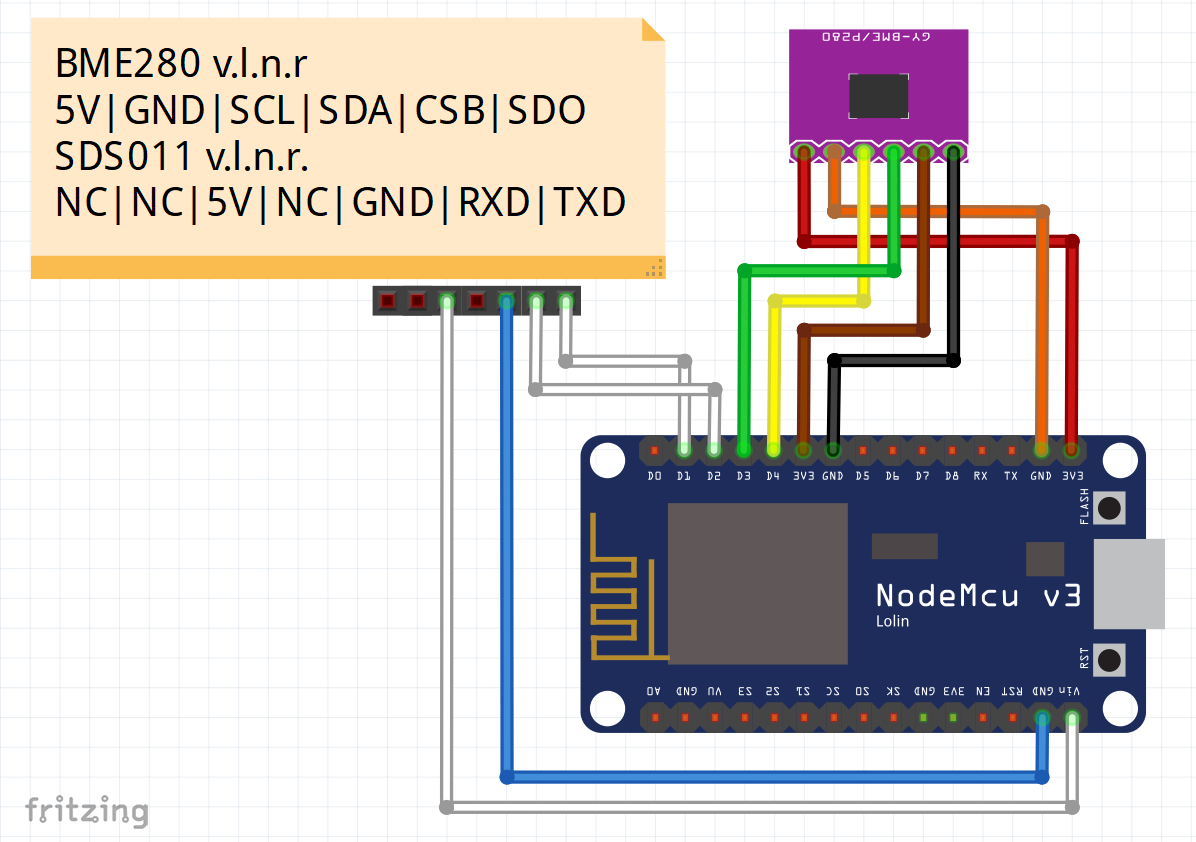
\includegraphics[width=0.7\linewidth]{./ressourcen/Prod_Verdrahtungsplan}
	\caption{Der Standard"=Verdrahtungsplan für den \sk}
	\label{fig:skwiringdefault}
\end{figure}

\subsection{Unit"=Tests}
Da in der \pg als Vorgehensmodell TDD festgelegt wurde, existieren für die \skfw Unit"=Tests.
Diese sind in der Ordnerstruktur unter \dirname{test} zu finden (siehe \Fref{sec:skFolderStructure}).
Die Testausführung geschieht ebenfalls über das \console{make.sh}"=Skript.
Dabei ist zu beachten, dass die Dateien \filename{config.json}, \filename{credentials.json} und die \filename{mergedConfig.json} im Ordner \dirname{config} vorhanden sind.
Die \filename{mergedConfig.json} ist dabei die zusammengefügte \filename{.json}"=Datei aus \filename{config.json} und \filename{credentials.json}.
Konfigurationsänderungen, beschrieben im Dokument III, Abschnitt 1.4.4, müssen somit ebenfalls in der \filename{mergedConfig.json} vorgenommen werden, da sonst die Unit"=Tests fehlschlagen.
Die Ausführung der Unit"=Tests geschieht dann im Repositorium der \skfw mit \console{./make.sh test}.
Zu empfehlen ist hierbei auch das vorhergehende Aufräumen der alten Build"=Artefakte mittels \console{./make.sh clean}.

\subsection{Code"=Aufbau}
Der Code"=Aufbau folgt im Wesentlichen der Architektur in \Fref{sec:skArchitektur}, jedoch sind einige Komponenten nicht in der Architektur enthalten, da sie gesondert zu behandeln sind.
Diese werden in diesem Abschnitt erläutert.

\subsubsection{Bootstrapper}
Der \code{Bootstrapper} ist dazu da, die Konfiguration aus der \filename{config.json} und \filename{credentials.json} zu verarbeiten und die benötigten Objekte daraus zu erstellen.
Jede Komponente aus der Architektur wird hier initialisiert.
Außerdem erzeugt der \code{Bootstrapper} den \code{Scheduler} zum Verwalten der Tasks und die \code{Sensornode} als übergeordnetes Objekt, das den \code{Scheduler} beinhaltet.
Plattformspezifische Initialisierungen werden durch Vererbung an den \code{NodeMcuBootstrapper} und \code{NativeBootstrapper} delegiert.

\subsubsection{SensorNode}
Die \code{SensorNode} war ursprünglich als Container für alle dynamischen Objekte gedacht.
Durch die Verwendung von \textit{Smart"=Pointern} und einer frühen Umstrukturierung der Code"=Basis dient die \code{SensorNode} nun nur noch dazu, den \code{Scheduler} aufzurufen.

\subsubsection{Scheduler}
Der \code{Scheduler} dient dazu, alle Tasks im \textit{Round"=Robin"=Verfahren} aufzurufen.
Dabei ruft er die \code{act()}"=Methode des aktiven Tasks solange auf, bis entweder der Zeitschlitz von \SI{25}{ms} verstrichen ist, oder der Task kein \code{ITask::State} \code{::busy} als Rückgabewert liefert.
Zusätzlich bricht der Scheduler die Ausführung der Tasks ab, sobald ein Task \code{ITask::State::error} als Rückgabewert liefert.
Dies hat einen Programmabbruch, oder im Falle der NodeMCU einen Neustart, zur Folge.

\subsubsection{Platform}
Das \code{Platform}"=Objekt dient als Abstraktionsschicht zu stellenweise benötigten plattformspezifischen Funktionen.
Diese werden durch Vererbung bereitgestellt.
Folgende Aufzählung listet Funktionalitäten auf:
\begin{itemize}
	\item \code{FileWrapper}: Operationen auf dem Dateisystem ausführen.
	\item \code{NodeMcuPlatformFactory}: Erzeugt den \code{FileWrapper}.
	\item \code{SerialWrapper}: Operationen auf der seriellen Schnittstelle ausführen.
	\item \code{NodeMcuServerConnectionFactory}: Erzeugt TCP"=Verbindungen (nicht in Native implementiert).
	\item \code{NodeMcuSystemStatusWrapper}: Liefert Statusinformationen zum System (nicht in Native implementiert).
\end{itemize}

\subsubsection{StringPool}
Das \code{StringPool}"=Objekt ist als Container für alle im Code verwendeten Strings vorgesehen.
Die Idee dahinter ist, dass alle Strings an einer Stelle gesammelt werden, um unnötige Duplikate im Speicher zu vermeiden.
Die Strings können im Code über \textit{enum}"=Werte und entsprechenden \code{get}"=Funktionen referenziert werden.
Als geplante, aber noch nicht implementierte, Funktionalität sollten die Strings entweder in den Programmspeicher, oder sogar in das Dateisystem, ausgelagert werden, um Speicherplatz im RAM zu sparen.
Durch die bislang geringe Anzahl an Strings wurde dies allerdings nicht umgesetzt.

\subsection{Firmware"=Updates}
In diesem Abschnitt werden die Firmware"=Updates behandelt.
Firmware"=Updates werden in der Develop-Umgebung per HTTP über den Server \url{https://pg-rio-strg.informatik.uni-oldenburg.de} bezogen.
\input{./dokument2/entwicklerdoku/skFirmwareUpdates}

\subsection{Code"=Konventionen}
In diesem Abschnitt werden die Code"=Konventionen beschrieben, die in dem \reponame{sensornode"=firmware}"=Repositorium verwendet werden.
In den anderen Repositorien aus \tbl{skfwrepos} gelten keine Code"=Konventionen.

\subsubsection{Code"=Styling}
Für das Styling des Codes wird das Tool clang"=format verwendet.
Die Definition der Formatierung ist in der Datei \filename{.clang"=format} im Wurzelverzeichnis des Projekts zu finden.
Die Korrektheit des Stylings wird durch den Jenkins"=Job überprüft und kann durch die Verwendung von \console{./make.sh format} oder die Verwendung von Extensions in VS Code (Clang"=Format ermöglicht die Formatierung beim Speichern einer Datei) angewandt werden.

\subsubsection{Namenskonventionen}
In diesem Projekt werden durchweg \textit{telling names} verwendet.
Das heißt die Namen von Variablen, Funktionen und Klassen sollten ihre Funktionalität möglichst genau beschreiben.
Dabei sollen die Namen aber so kurz wie möglich, aber so lang wie nötig gehalten werden.
Darüberhinaus gibt es folgende Konventionen zur Benennung innerhalb dieses Projekts:

\begin{itemize}
	\item Sind in Klassen, die nicht von \code{ITask} ableiten, Arbeitsaufrufe notwendig, so sind diese Funktionen mit \code{act()} zu benennen. (Im Gegensatz zum \code{call()} in \code{ITask})
	\item Werden \code{unique\_ptr<T>} durch Funktionen an einen neuen Owner übergeben, so ist die Funktion mit \code{take\textit{Something}()} zu benennen.
	\item Erfolgt eine Kommunikation mit einer Klasse, die als State Machine implementiert ist, welche den internen Zustand der State Machine ändert, so ist die Funktion mit \code{trigger\textit{Something}()} zu benennen.
\end{itemize}

\subsubsection{C/C++"=Konventionen}
Folgende C/C++"=Konventionen sollten befolgt werden:

\begin{itemize}
	\item In \code{for}"=Schleifen wird der Inkrement"=Operator \code{++i} (nicht \code{i++}) verwendet.
	\item Es werden durchweg smart pointers (gegenüber raw pointers) verwendet. Siehe Guidelines.
	\item Es werden \textit{enum classes} verwendet, siehe z.B. \code{DataSinkNames} im Projekt.
	\item Bei überschriebenen Methoden ist \code{override} bzw. \code{final} zu ergänzen.
	\item State Machines werden mit \code{std::function} implementiert. Dies ist vor allem beim Refactoring vorhandener State"=Machines im \code{switch/case}"=Style zu beachten.
\end{itemize}

Ausnahmen von diesen Regeln, sind mittels Code"=Kommentar zu begründen.
Des Weiteren wurden die Regeln im Laufe der \pg erweitert, sodass sie nicht durchgehend Anwendung fanden.

\subsubsection{C++"=Guidelines}
\begin{itemize}
	\item \url{http://isocpp.github.io/CppCoreGuidelines/CppCoreGuidelines}
	\item \url{https://www.heise.de/developer/artikel/C-Core-Guidelines-Interfaces-I-3767608.html}
	\item \url{https://www.heise.de/developer/artikel/C-Core-Guidelines-Regeln-fuer-Smart-Pointer-3919901.html}
\end{itemize}

\subsection{Steps to Debug}
Für das Debugging gibt es zwei vorgesehene Möglichkeiten.
Die erste ist das Ausführen der Sensorknoten"=Software auf dem Entwicklerrechner.
Dabei können die Debug"=Funktionalitäten von Visual Studio Code verwendet werden.
Der Nachteil dieser Variante ist, dass nicht die Produktivsoftware vollumfänglich getestet werden kann.
Also können nicht alle Fehler aufgedeckt werden (insbesondere Fehler im plattformspezifischen Code).
Bei der zweiten Variante werden Debug"=Ausgaben in den Code eingebunden, um das Verhalten des Programms auf dem Sensorknoten zu analysieren.
Die Debug"=Firmware kann dann mit \console{./make.sh nodemcu\_v2\_debug} \console{ \&\& ./make.sh nodemcu\_v2\_debug\_upload} erzeugt und auf den Sensorknoten eingespielt und gestartet werden.
Zudem muss der PIN D4 der NodeMCU an einen USB"=Serial"=Converter angeschlossen werden (siehe \Fig{skwiringdebug}), um die Debug"=Ausgaben (115200 Baud, 8N1) am Rechner anzeigen zu können.
Diese Variante ist aufwändiger, aber kann auch Fehler im NodeMCU"=spezifischen Code aufdecken.

\begin{figure}[htb]
	\centering
	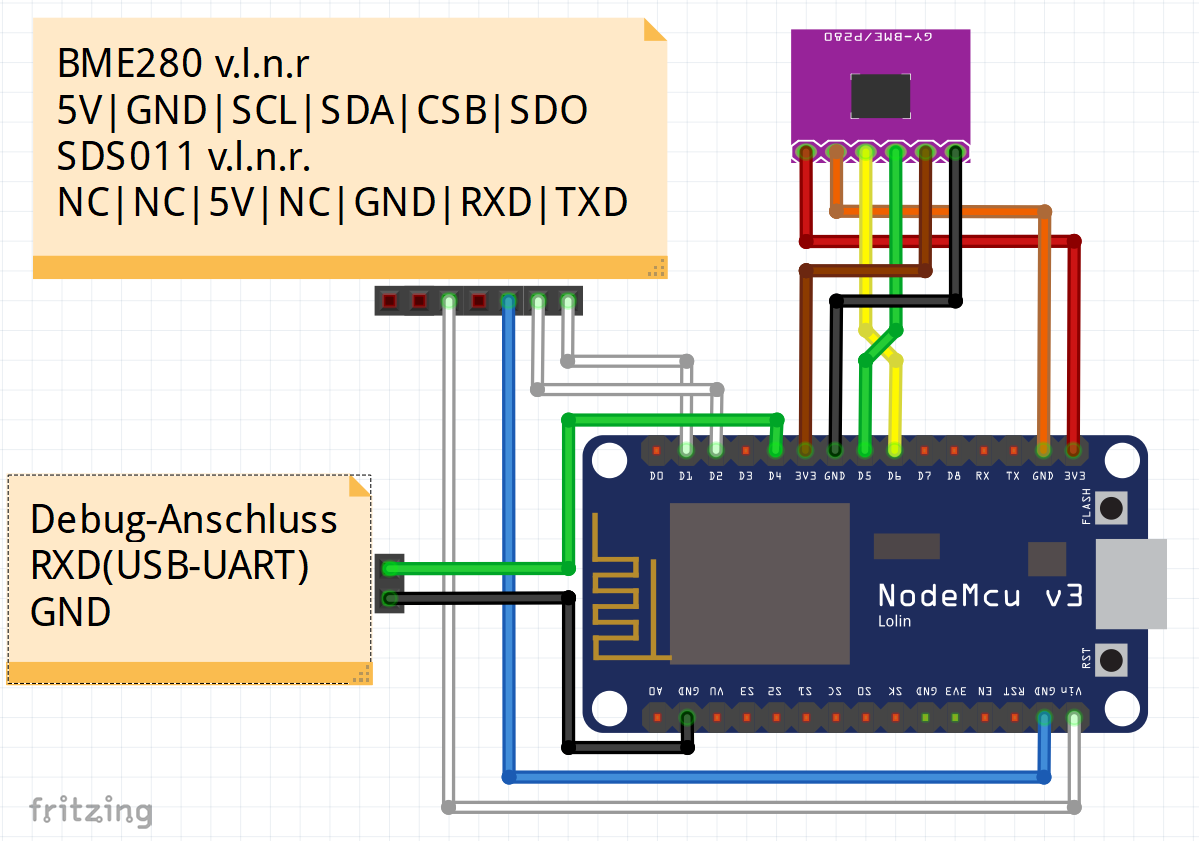
\includegraphics[width=0.7\linewidth]{./ressourcen/Prod_Verdrahtungsplan_Debug}
	\caption{Der Debug"=Verdrahtungsplan für den \sk}
	\label{fig:skwiringdebug}
\end{figure}

\subsection{Dokumentation}
In diesem Abschnitt werden die Dokumentationsrichtlinien für die \skk behandelt.
Diese teilen sich in die Code"=Dokumentation und Architektur auf.

\subsubsection{Code"=Dokumentation}
Die Codedokumentation der Interfaces und Klassen erfolgt in den zugehörigen h"=Dateien.
Es muss mindestens eine Beschreibung zum Interface bzw. der Klasse angegeben und darüber hinaus alle öffentlichen Funktionen und Enums dokumentiert werden.
Konstruktoren und Destruktoren werden nur im Ausnahmefall erläutert.
Aus den Codekommentaren wird mittels Doxygen automatisch eine Dokumentation im HTML"=Format generiert.
Dazu wird der Befehl \console{./make.sh code\_docu} verwendet.
Zudem wird die Dokumentation bei der Ausführung des Jenkins"=Jobs erstellt und als Artefakt in einer ZIP"=Datei archiviert.

\subsubsection{Architektur}
\label{sec:skArchitektur}
Die Dokumentation der Architektur der \skfw wird im Repositorium \reponame{dokumentation}\footnote{\url{https://git.swl.informatik.uni-oldenburg.de/projects/PGRIO/repos/dokumentation/browse}} vorgenommen.
Dort sind zum einen die Beschreibung der Architektur, die sich als Fließtext in den Gesamttext einfügt, und zum anderen im Unterverzeichnis \dirname{ressourcen} die UML"=Modelle zu finden.

Bei Änderungen an der Architektur wird die Dokumentation immer zusammen mit der Implementierung (innerhalb des selben JIRA"=Tickets) gepflegt.

\subsection{Konfigurationstool}
Das PGRIO"=SK"=Config"=Tool ist ein Windows"=Programm zur Installation und Konfiguration der Firmware für den Sensorknoten der Projektgruppe RiO.
Mit dem Tool kann die aktuelle Firmware aus dem Internet heruntergeladen und auf dem ESP8266 geflasht werden.
Zusätzlich können Konfigurationsänderungen auf dem Sensorknoten vorgenommen werden.

\subsubsection{Technologie}
Dieses Projekt wird mit C\# und dem .NET"=Framework 4.7.2 mit Hilfe von WPF entwickelt.

\subsubsection{Entwicklungsumgebung}
Als Entwicklungsumgebung kommt die Community"=Edition von MS Visual Studio zum Einsatz.

\subsubsection{Deployment}
Es ist kein CI/CD"=Job für dieses Projekt angelegt.
Daher muss ein Deployment manuell durchgeführt werden.
Dazu wird das Projekt mit Visual Studio gebaut und die PGRIO"=SK"=Config"=Tool.exe am gewünschten Pfad veröffentlicht.
Die Produktiv"=Version wird auf der Website \url{https://pg-rio-uis.informatik.uni-oldenburg.de/mitmachen} als Download bereitgestellt.
Die exe"=Datei ist eigenständig (ohne zugehörige dll"=Dateien) ausführbar.

\subsubsection{Abhängigkeiten}
Es gibt die in \Tbl{skctdependencies} dargestellten Abhängigkeiten im Projekt.

\begin{table}[htb]
	\caption{Externe Abhängigkeiten des Konfigurationstools}
	\begin{tabular}{|p{0.14\linewidth}|p{0.20\linewidth}|p{0.07\linewidth}|p{0.08\linewidth}|p{0.14\linewidth}|p{0.20\linewidth}|}
		\hline
		Name & Verweis & Lizenz & Version & Einbindung & Erläuterung \\ \hline
		Caliburn. Micro & \url{https://caliburnmicro.com} & MIT & 3.2.0 & nuget"=Paket & Framework für DataBindings mit MVVM"=Pattern in WPF \\ \hline
		Crc32.NET & \url{https://github.com/force-net/Crc32.NET} & MIT & 1.2.0 & nuget"=Paket & Framework zur Berechnung einer CRC32"=Prüfsumme \\ \hline
		esptool"=ck & \url{https://github.com/igrr/esptool-ck} & GPL-2.0 & 0.4.13 & .exe als Embedded"=Resource & Tool zum Flashen der Firmware auf den ESP8266 \\ \hline
		NewtonSoft. Json & \url{https://www.newtonsoft.com/json} & MIT & 12.0.2 & nuget"=Paket & Framework zum Verarbeiten von JSON \\ \hline
	\end{tabular}
	\label{tbl:skctdependencies}
\end{table}


\section{Virtueller Sensorknoten}
Um die Funktionalität der einzelnen Komponenten des PG RiO Projektes zu testen, wurden virtuelle Sensorknoten implementiert. 
Die Entwicklerdokumentation des virtuellen Sensorknotens umfasst alle nötigen Informationen, die ein Entwickler für die Weiterentwicklung benötigt. 
Diese umfasst die Projektstruktur, die verwendeten externen Bibliotheken sowie eine Anleitung zum Aufsetzen des Projektes auf dem lokalen Rechner des Entwicklers. Des Weiteren wird in diesem Kapitel eine Anleitung gegeben, wie ein Entwickler eine neue Strategie für einen virtuellen Sensorknoten implementieren kann.

\subsection{Projektstruktur}
In diesem Abschnitt wird die Projektstruktur näher erläutert. Dazu zählt das verwendetete Repositorium sowie die externen Abhängigkeiten, die im folgenden erläutert werden.

\subsubsection{Repositorium}
Dieser Abschnitt bezieht sich auf das Repositorium, das für die virtuellen Sensorknoten verwendet wird:
\begin{enumerate}
	\item Git öffnen
	\item Das folgende Repositorium muss geklont werden 
	\begin{itemize}
		\item https://git.swl.informatik.uni-oldenburg.de/scm/pgrio/virtual-sensor.git
	\end{itemize}
\end{enumerate}
Für die virtuellen Sensorknoten exisitieren Strategien, die innerhalb dieses Repositoriums implementiert wurden. 

\subsubsection{Externe Abhängigkeiten}
In diesem Abschnitt werden die genutzten Frameworks aufgelistet.
\begin{table}[htb]
	\begin{tabular}{|p{0.14\linewidth}|p{0.14\linewidth}|p{0.20\linewidth}|p{0.20\linewidth}|p{0.20\linewidth}|}
		\hline
		Name & Version & Lizenz & Link & Grund \\ \hline
		@hapi/joi & 15.0.2 & BSD-3-Clause & \url{https://www.npmjs.com/package/@hapi/joi} & Validierung der Konfigurations-Dateien\\ \hline
		mqtt & 2.18.8 & MIT & \url{https://www.npmjs.com/package/mqtt} & Nutzung des Mqtt-Protokolls \\ \hline
	\end{tabular}
\end{table}

\subsection{Steps to Code}
In diesem Abschnitt wird erläutert, wie ein Entwickler zum Projekt beitragen kann. Im folgenden werden die notwendigen Schritte aufgelistet: 
\begin{enumerate}
	\item Zugriff auf das \textit{virtual-sensor} Repositorium erlangen
	\item textbf{Installation der Abhängigkeiten} \newline
	Die nötigen Bibliotheken und externen Abhängigkeiten werden durch den Befehl \console{npm install} installiert.
	\item Programmieren 
	\item \textbf{Starten der Anwendung} \newline
	Die Anwendung kann in verschieden Arten gestartet werden: Im Entwicklermodus oder im "Watch""=Modus. Dafür dienen die jeweiligen Befehle \console{npm run start} und \console{npm run start:dev}.
	\item \textbf{Testen der Anwendung} \newline
	Damit die Anwendung getestet werden kann stehen Unit"=Tests und Integrationstests (E2E) zur Verfügung. 
	Diese können durch einen einfachen Befehle ausgeführt werden: \console{npm run test}.
\end{enumerate}

\subsection{Implementierung einer neuen Strategie}
In diesem Abschnitt wird erklärt wie ein Entwickler eine neue Strategie für einen virtuellen Sensorknoten implementieren kann.
 Wenn eine neue Strategie implementiert wird müssen folgende Methoden implementiert werden:
	\begin{enumerate}
		\item function Strategy() {} //Der Konstruktor der neuen Strategie
		\item Strategy.prototype.end = function() {} //Die End-Funktion wird genutzt um die Strategie zu beenden.
		\item Strategy.prototype.execute = function() {} // Die Execute-Funktion wird genutzt um die Strategie zu starten. Sie sollte niemals Argumente übernehmen.
	\end{enumerate}
Im Folgenden wird beschrieben wird die Konfiguration für die neue Strategie hinzugefügt wird:
	\begin{enumerate}
		\item Erweiterung der \textit{validateConfig} Funktion des \textit{configurationLoader.js} um die neue Strategie.
		\item Erweiterung der \textit{loadConfiguration} Funktion des \textit{configurationLoader.js} um die neue Strategie.
	\end{enumerate}
Für die Registrierung der neuen Strategie an der Hauptanwendung sind folgende Schritte notwendig:
	\begin{enumerate}
		\item Erweiterung der \textit{loadConfiguration.js} des \textit{MqttHandler.js}, um die neue Strategie nutzen zu können.
	\end{enumerate}


\subsection{Steps to Deploy}
In diesem Abschnitt wird näher erläutert, wie der aktuelle Stand des Repositoriums auf Docker-Hub veröffentlich wird.
\begin{enumerate}
	\item Bauen des Docker-Images durch ausführen von folgendem Befehl in der Kommandozeile: docker build -t pgrio/virtual-sensor .
	\item Docker-Image lokal starten durch ausführen von folgendem Befehl in der Kommandozeile: docker run --rm -it pgrio/virtual-sensor:latest
\end{enumerate}



\section{IoT-Plattform}
Die Entwicklerdokumentation für die IoT"=Plattform von der PG RiO fasst alle relevanten Information zusammen, die für die Weiterentwicklung der einzelnen Komponenten benötigt werden.
Dazu gehören die verwendeten Repositorien, die externen Bibliotheken, Steps to Code, die Code-Konventionen, die Steps to Debug und die Code-Dokumentation. 

\subsection{Repositorien}
In diesem Abschnitt wird die Projektstruktur der IoT"=Plattform genauer erläutert. Dazu zählen die Repositorien, die in \Fref{sec:iot:repositorien} genauer erläutert sind, und eine Liste aller externen Abhängigkeiten in \Fref{sec:iot:extAbh}.

\subsubsection{Projekte}
\label{sec:iot:repositorien}
In diesem Abschnitt werden alle verwendeten Repositorien der IoT"=Plattform beschrieben. Einige Projekte der IoT"=Plattform basieren auf dem TypeScript Framework NestJS und können alle durch die gleichen Befehle weiterentwickelt werden. Eine Anleitung für die Weiterentwicklung ist in \Fref{sec:iot:stepstocode} einsehbar. Dies betrifft die nachfolgenden Projekte:
\begin{itemize}
	\item iot"=api"=gateway
	\item iot"=identity"=service
	\item iot"=microservice"=humidity
	\item iot"=microservice"=pm10
	\item iot"=microservice"=pm25
	\item iot"=microservice"=pressure
	\item iot"=microservice"=sv
	\item iot"=microservice"=temp
	\item iot"=microservice"=template
	\item iot"=microservice"=uis
\end{itemize}
Eine genaue Beschreibung der einzelnen Komponenten kann der Architekturdokumentation entnommen werden. 
Das Ziel dieser Repositorien kann in \Tbl{iotrepos}  gefunden werden.

\subsubsection{Externe Abhängigkeiten}
\label{sec:iot:extAbh}
Eine vollständige Tabelle samt Lizenzen, Links und Erläuterung ist der folgenden Liste zu entnehmen:
\begin{itemize}
	\item \textbf{iot"=api"=gateway}, \Tbl{dependenciesApiGateway} 
	\item \textbf{iot"=collection"=creater}, \Tbl{dependenciesCollectionCreater} 
	\item \textbf{iot"=data"=collector}, \Tbl{dependenciesDataCollector}
	\item \textbf{iot"=identity"=service}, \Tbl{dependenciesIdentityService}
	\item \textbf{iot"=microservice"=pm10}, \Tbl{dependenciesMicroPM10}
	\item \textbf{iot"=microservice"=pm25}, \Tbl{dependenciesMicroPM25}
	\item \textbf{iot"=microservice"=temp}, \Tbl{dependenciesMicroTemp}
	\item \textbf{iot"=microservice"=sv}, \Tbl{dependenciesMicroSV}
	\item \textbf{iot"=microservice"=uis}, \Tbl{dependenciesMicroUIS}
\end{itemize}

\subsection{Steps to Code}
\label{sec:iot:stepstocode}
In diesem Abschnitt wird das Vorgehen beschrieben, wie ei Entwickler zu dem Projekt beitragen kann. Die folgenden Schritte sind dafür notwendig: \newline
\begin{enumerate}
	\item Als Editor für die Entwicklung der IoT"=Plattform wurde Visual Studio Code genutzt. Daher sollte zuerst der Editor installiert werden. Unter folgenden Link:
	\begin{itemize}
		\item https://code.visualstudio.com/download
	\end{itemize}
	\item Alle Komponenten der IoT"=Plattform sind mit dem Framework NestJS entwickelt worden. Daher muss sichergestellt sein, dass Node.js installiert ist. Unter folgenden Link kann Node.js installiert werden: 
	\begin{itemize}
		\item{https://nodejs.org/en/}
	\end{itemize}
	\item Nach erfolgreicher Installation von Node.js kann die NestJS CLI installiert werden. Für die Installation kann das Terminal im Editor verwendet werden. Dafür ist folgender Befehl in der Kommandozeile nötig: 
	\begin{itemize}
		\item{\console{npm i -g @nestjs/cli}}
	\end{itemize}
	\item Da einige Komonenten der IoT"=Plattform Schnittstellen bereitstellen und auf eine Datenbank zugreifen ist es notwendig eine Datenbank installiert zu haben. Zum einen kann sich lokal mit einer Testdatenbank verbunden werden und zum anderen kann, nach die Plattform deployed ist, auf die Datenbank zugegriffen werden. Eine Anleitung zum Verbinden sowie Testen der Projekte mit der Datenbank wird in \Fref{sec:iot:stepstodebug} beschrieben. Unter folgendem Link steht der Download für die Datenbank bereit: 
	\begin{itemize}
		\item {https://www.mongodb.com/download-center/community}
	\end{itemize}
	\item Es ist empfehlenswert ein entsprechendes Tool für die MongoDB zu installieren. Unter folgendem Link steht der Download für MongoDB Compass bereit. 
	\begin{itemize}
		\item {https://www.mongodb.com/download-center/compass}
	\end{itemize}
	\item Außerdem wird für das Deployment der IoT"=Plattform Docker verwendet. Daher sollte, zum Überprüfen von lokalen Projekten, Docker installiert sein. Eine Anleitung, wie eine Projekt mit Docker getestet werden kann, kann in \Fref{sec:iot:stepstodebug} gefunden werden. Unter folgendem Link ist eine Anleitung zur Installation von Docker zu finden: 
	\begin{itemize}
		\item {https://docs.docker.com/docker-for-windows/install/}
	\end{itemize}
	\item Einige Projekte der IoT"=Plattform verbinden sich mit dem MQTT Broker, um beispielsweise Daten der Sensorknoten zu erhalten. Daher kann zum Testen eines Projektes ein MQTT Client verwendet werden. Unter folgendem Link steht der MQTT Explorer Download bereit. Mit diesem kann sich auf den MQTT Broker der PG RiO eingeloggt werden: 
	\begin{itemize}
		\item {http://mqtt-explorer.com}
	\end{itemize}
	\item Visual Studio Code starten und anfangen zu Programmieren.
\end{enumerate}

\subsection{Code-Konventionen}
In diesem Abschnitt werden die Code-Konventionen beschrieben, die in den Repositorien der IoT"=Plattform verwendet werden. Zum einen wird ein Code Formatierer verwendet und zum anderen ein Tool, das den Code auf Lesbarkeit, Wartbarkeit und Funktionsfehler prüft. \newline
Mit dem Kommandobefehl \console{npm run format} wird der Code Formatierer \textit{prettier} durchgeführt. Somit wird das ganze Projekt richtig formatiert. \newline
Für die Überprüfung des Codes wird das Tool TSLint verwendet. Der Kommandobefehl lautet \console{npm run lint}. Alle Fehler werden nach Ausführung des Befehls angezeigt. Die gesamte Liste der Regeln können unter https://palantir.github.io/tslint/rules/ gefunden werden.

\subsection{Steps to Debug}
\label{sec:iot:stepstodebug}
In diesem Abschnitt wird unter \Fref{sec:iot:lokal} erklärt, wie die einzelnen Projekte lokal aufgesetzt und deren Funktionalität getestet werden kann. Außerdem kann in \Fref{sec:iot:dockerdepl} eine Anleitung zum Deployment der gesamten IoT"=Plattform auf der Development Umgebung gefunden werden.
\subsubsection{Lokale Anwendung}
\label{sec:iot:lokal}
In diesem Abschnitt wird erklärt, wie die einzelnen Repositorien lokal gestartet werden können und welche Einstellungen dafür vorgenommen werden müssen. Da die meisten Projekte der IoT"=Plattform mit Typescript entwickelt wurden, können folgende Befehle für diese Projekte ausgeführt werden: \newline 
\textbf{Installation der Abhängigkeiten} \newline
Die nötigen Bibliotheken und externen Abhängigkeiten werden durch den Befehl \console{npm install} installiert.
\textbf{Starten der Anwendung}\newline
Die Anwendung kann in verschieden Arten gestartet werden: Im Entwicklermodus, im "Watch""=Modus oder im Produktionsmodus. Dafür dienen die jeweiligen Befehle \console{npm run start}, \console{npm run start:dev} und \console{npm run start:prod}. 

\textbf{Testen der Anwendung}\newline
Damit die Anwendung getestet werden kann stehen Unit"=Tests und Integrationstests (E2E) zur Verfügung. 
Diese können durch die zwei einfachen Befehle ausgeführt werden: \console{npm run test} und \console{npm run test:e2e}.

Diese Befehle sind für die folgenden Projekte ausführbar: 
\begin{itemize}
	\item iot-api-gateway
	\item iot-api-prototyp
	\item iot-identity-service
	\item iot-microservice-pm25
	\item iot-microservice-pm10
	\item iot-microservice-uis
	\item iot-microservice-sv
	\item iot-microservice-temp
\end{itemize}

Für die folgenden Projekte sind diese Befehle nicht ausführbar, weil diese mit Javascript implementiert wurden: 
\begin{itemize}
	\item iot-collection-creater
	\item iot-data-collector
\end{itemize}
Die folgenden Befehle sind für die beiden Projekte anwendbar: \newline
\textbf{Installation der Abhängigkeiten} \newline
Die nötigen Bibliotheken und externen Abhängigkeiten werden durch den Befehl \console{npm install} installiert.

\textbf{Starten der Anwendung}\newline
Die Anwendung kann in verschieden Arten gestartet werden: Im Entwicklermodus oder im "Watch""=Modus. Dafür dienen die jeweiligen Befehle \console{npm run start} und \console{npm run start:dev}.

\textbf{Testen der Anwendung}\newline
Damit die Anwendung getestet werden kann stehen Unit"=Tests und Integrationstests (E2E) zur Verfügung. 
Diese können durch einen einfachen Befehle ausgeführt werden: \console{npm run test}. Allerdings sind lediglich für das Projekt \textit{iot-data-collector} Tests vorhanden, sodass diese Befehle nur für dieses Projekt ausführbar sind. \newline

Da die Projekte der IoT"=Plattform auf Docker Hub veröffentlicht werden können folgende Befehle für alle Projekte der IoT"=Plattform ausgeführt werden: \newline
\textbf{Docker} 
\begin{enumerate}
	\item Für das Deployment der IoT"=Plattform wurde Docker ausgewählt. Um den aktuellen Stand eines lokalen Projekts auf Docker Hub zu veröffentlichen ist zunächst ein Login über das Terminal notwendig: \newline
	\console{docker login}
	Die geforderten Login Daten können nun eingegeben werden. 
	\item Zuerst muss ein Image erstellt werden: \newline
	\console{docker build -t pgrio/iot-testprojekt}
	\item Danach kann das Image gestartet werden: \newline
	\console{docker run -p 49160:8080 -d pgrio/iot-testprojekt}
	\item Außerdem kann das Image versioniert werden: \newline
	\console{docker tag \textit{imageid} pgrio/iot-testprojekt:tag}
	\item Danach kann das Image auf Docker Hub veröffentlicht werden: \newline
	\console{docker push pgrio/iot-testprojekt}
	\item Mit folgendem Befehlt können alle aktiven Container angezeigt werden: \newline
	\console{docker ps}
	\item Um einen Container zu stoppen muss folgender Befehl ausgeführt werden: \newline
	\console{docker stop \textit{containername}}
	\item Ein Image kann mit folgendem Befehl von Docker Hub bezogen werden: \newline
	\console{docker pull pgrio/iot-testprojekt} 
\end{enumerate}

Damit die Funktionalität der Projekte getestet werden kann, wird im folgenden für jedes Projekt die zusätzliche Konfiguration beschrieben. \newline
Da jedes der Projekt eine Verbindung zur Datenbank aufbaut, um zum Beispiel Daten abzufragen, muss die \textit{.env} Datei angepasst werden. In \Fref{sec:iot:stepstocode} wurde bereits darauf verwiesen, dass eine MongoDB installiert sein muss. Außerdem werden in den \textit{env.} Dateien Zugangsdaten für die Authentifizierung angegeben. Diese Zugangsdaten müssen mit denen in der Datenbank übereinstimmen. Außerdem werden für einige Projekte in den \textit{env.} Dateien die Zugangsdaten für den MQTT Broker hinterlegt, die ebenfalls mit denen aus der Datenbak übereinstimmen müssen. Anderenfalls würden beim Start eines Projektes Fehler ausgegeben werden. \newline
Die \textit{development.env} Datei der Microservices sind identisch: \newline
\begin{lstlisting}[language=json,firstnumber=1,basicstyle=\footnotesize]
DB_URL = mongodb://localhost:27017/test-db
API_GATEWAY_URL = http://localhost:8080
SERVICE_USERNAME = MicroserviceTest
SERVICE_PASSWORD = MicroservicetestPassword
RENEW_INTERVALL = 5
SERVICE_PORT = 3002
\end{lstlisting}
Für das API-Gateway sieht die \textit{development.env} Datei wie folgt aus: \newline
\begin{lstlisting}[language=json,firstnumber=1,basicstyle=\footnotesize]
IDENTITY_SERVICE_URL = http://192.168.99.100:9090
SERVICE_LEASE_DURATION = 30
JWT_EXP_DURATION = 3600
JWT_SIGNER = PGRIO
DB_URL = mongodb://localhost:27017/test-db
\end{lstlisting}
Für den Identity Service sieht die \textit{development.env} Datei wie folgt aus: \newline
\begin{lstlisting}[language=json,firstnumber=1,basicstyle=\footnotesize]
DB_URL=mongodb://192.168.99.100:27017/iot-platform
\end{lstlisting}
Für die Projekte \textit{iot-data-collector} und \textit{iot-collection-creater} sind keine \textit{development.env} Dateien nötig sondern \textit{config.env} Dateien. Für den Data-Collector sieht die \textit{config.env} Datei wie folgt aus: \newline
\begin{lstlisting}[language=json,firstnumber=1,basicstyle=\footnotesize]
MQTT_BROKER_URL=mqtt://testbroker.de
MQTT_USERNAME=pgrio-datacollector
MQTT_PASSWORD=pgrio-datacollector
MQTT_CLIENTID=pgrio-datacollector-test
DB_URL=mongodb://localhost:27017/test-db
\end{lstlisting}
Für den Collection-Creater sieht diese wie folgt aus: \newline
\begin{lstlisting}[language=json,firstnumber=1,basicstyle=\footnotesize]
DB_URL=mongodb://localhost:27017/test-db
\end{lstlisting}
Nachdem die \textit{env.} Dateien anglelegt und angepasst wurden kann ein beliebiges Projekt gestartet werden. Im folgenden werden die einzelnen Funktionalitäten der Projekte erläutert und wie diese getestet werden können. \newline
\textbf{Collection-Creater}\newline
Der Collection hat die Aufgabe sich mit der Datenbank zu verbinden und alle Collections mit deren Validierungsregeln zu erstellen. Nachdem das Projekt gestartet wurde und sich das Programm beendet hat sind in der Datenbank, die in der \textit{config.env} Datei angegeben wurde, alle Collections erstellt. Anhand des Datenbankschemas sowie des Skripts können die Validierungsregeln eingesehen werden. Es ist nur erlaubt ein Objekt zu einer Collection hinzuzufügen, die den Regeln entspricht. \newline
\textbf{API Gateway und Identity Service}\newline
Das API Gateway und der Identity Service können sehr gut zusammen getestet werden. Die beiden Projekte können gestartet werden. In der Test Datenbank können nun Zugangsdaten für einen externen Service hinterlegt werden. Da zuvor das Skript zum Erstellen sowie Validieren der Einträge ausgeführt wurde, sind nun alle Collections verfügbar. Eine manuelle Eingabe der Daten kann also erfolgen.  Nach erfolgreichem Start der beiden Projekte können nun zum Beispiel die Endpunkte des API Gateways getestet werden. Dazu gehört beispielsweise das Erhalten eines JWT Tokens oder das Abfragen aller aktiven Microservices. Zu beachten ist, dass die Datenbank für die entsprechenden Abfragen korrekt befüllt sein muss. Alle Schnittstellen können in der Architekturdokumentation in Dokument 1 gefunden werden. \newline
\textbf{Microservices}\newline
Die Microservices können auf zwei Arten getestet werden. Zum einen kann die Authentifizierung am API Gateway getestet werden und zum anderen kann die Abfrage von Daten getestet werden. Zu beachten ist, dass die Zugangsdaten, also Username und Passwort, in der Datenbank mit denen in der \textit{development.env} Datei übereinstimmen muss. \newline
Zunächst kann die Authentifizierung am API Gateway getestet werden, indem die entsprechenden Zugangsdaten in der Datenbank hinterlegt wurden. Danach müssen die Projekte \textit{iot-identity-service}, \textit{iot-api-gateway} und der entsprechende Microservice gestartet werden. Nach erfolgreichem Start kann die Abfrage aller aktiven Microservices am API Gateway getestet werden. \newline
Außerdem können die entsprechenden Endpunkte getestet werden. Dafür können die Abfragen über das API Gateway erfolgen oder direkt beim Service abgefragt werden. Zu beachten ist, dass für jede Abfrage die entsprechende Collection in der Datenbank gefüllt sein muss. Die Schnittstellen, die die einzelnen Microservices anbieten sind im Dokument 1 unter der Architektur zu finden. \newline
\textbf{Data-Collector}\newline
Der Data Collector hat die Aufgabe die Daten der Sensorknoten über den MQTT Broker anzunehemen und persistent in der Datenbank zu speichern. Da die \textit{env.} Datei bereits angepasst ist muss lediglich das Projekt gestartet werden. Außerdem kann sich auf den MQTT Broker eingeloggt werden, um sicherzustellen, dass die richtigen Daten gespeichert werden. Eine Anleitung dafür wurde bereits in \ref{sec:sk:stepsToCode} gegeben. Sobald das Projekt gestartet wurde, werden die Daten des MQTT Brokers in der lokalen Test Datenbank gespeichert. 

\subsubsection{Deployment auf Development Umgebung}
\label{sec:iot:dockerdepl}
Damit nun die ganze IoT"=Plattform in der Development Umgebung gestartet werden kann, wird docker-compose verwendet. Die folgenden Schritte sind zum Starten der IoT"=Plattform mit docker-compose nötig: 
\begin{enumerate}
	\item Zuerst muss sich der Entwickler auf die VM einloggen
	\item Danach müssen die \textit{env.} Datein angelegt oder gegebenenfalls angepasst werden. Die \textit{env.} Dateien wurden bereits in \Fref{sec:iot:lokal} erläutert. \newline
	Beispielsweise müsste eine neue \textit{env.} Datei angelegt werden, wenn ein neues Microservice deployed werden soll. Unter \textit{home/pgrio/microservices/} muss nun ein neuer Ordner BeispielMicroservice angelegt werden, der die \textit{env.} Datei enthält \newline
	Die \textit{env.} Datei muss den folgenden Inhalt haben: \newline
	\begin{lstlisting}[language=json,firstnumber=1,basicstyle=\footnotesize]
	DB_URL = DevelopmentDatenbankURL
	API_GATEWAY_URL = DevelopmentAPIGatewayURL
	SERVICE_USERNAME = BeispielMicroservice
	SERVICE_PASSWORD = BeispielMicroservicePassword
	RENEW_INTERVALL = 5
	SERVICE_PORT = 3102
	SERVICE_HOST = beispielmicroservice
	\end{lstlisting}
	\begin{itemize}
		\item DB\_URL: URL der Datenbank, die auf dem Development"=System läuft
		\item API\_GATEWAY\_URL: URL des API Gateways, das auf dem Development"=System läuft
		\item SERVICE\_USERNAME: Der Benutzername des Microservices, der auch in der Datenbank hinterlegt ist
		\item SERVICE\_PASSWORD: Das Passwort des Microservices, das auch in der Datenbank hinterlegt ist
		\item SERVICE\_PORT: Der Port des Microservices, auf dem der Microservice erreichbar ist. Dieser ist nur dür das API Gateway offen und nicht außerhalb des Docker Netzwerkes
		\item RENEW\_INTERVAL Das Zeitintervall, in dem der Microservice ein neues Token anfragt
		\item SERVICE\_HOST: Entspricht dem Namen des Microservices in der yaml Datei und ist notwendig, damit das API Gateway die Anfragen, an der richtigen Microservice weiterleiten kann
	\end{itemize}
	\item Nachdem die \textit{env.} Dateien erstellt wurden muss die yaml Datei angepasst werden. Für das zuvor genannte Beispiel, einen neuen Microservice zu deployen, ist die Anpassung der yaml Datei ab Zeile 85 notwendig. Folgend ist die aktuelle yaml Datei der Developmentumgebung gezeigt: \newline
	\begin{lstlisting}[language=json]
	version: '3.5'
	services:
	mqttbroker:
	image: pgrio/iot-mqtt-broker-hive:latest
	volumes:
	- /home/pgrio/iot-platform/mqtt/config.properties:/opt/hivemq/config.properties
	ports:
	- "127.0.0.1:1883:1883"
	restart: always
	depends_on:
	- identityservice
	identityservice:
	image: pgrio/iot-identity-service:latest
	volumes:
	- /home/pgrio/iot-platform/identityservice/production.env:/usr/src/app/production.env
	environment:
	- NODE_ENV=production
	expose:
	- "9090"
	restart: always
	depends_on:
	- collection_creater
	api_gateway:
	image: pgrio/iot-api-gateway:latest
	volumes:
	- /home/pgrio/iot-platform/apigateway/production.env:/usr/src/app/production.env
	environment:
	- NODE_ENV=production
	ports:
	- "127.0.0.1:8080:8080"
	restart: always
	depends_on:
	- identityservice
	iot-data-collector:
	image: pgrio/iot-data-collector:latest
	volumes:
	- /home/pgrio/iot-platform/datacollector/config.env:/usr/src/app/config.env
	environment:
	- NODE_ENV=production
	restart: always
	depends_on:
	- collection_creater
	collection_creater:
	image: pgrio/iot-collection-creater:latest
	volumes:
	- /home/pgrio/iot-platform/collectioncreater/config.env:/usr/src/app/config.env
	environment:
	- NODE_ENV=production
	pm25microservice:
	image: pgrio/iot-microservice-pm25:latest
	expose:
	- "3000"
	volumes:
	- /home/pgrio/iot-platform/microservices/pm25/production.env:/usr/src/app/production.env
	environment:
	- NODE_ENV=production
	restart: always
	tempmicroservice:
	image: pgrio/iot-microservice-temp:latest
	expose:
	- "3004"
	volumes:
	- /home/pgrio/iot-platform/microservices/temp/production.env:/usr/src/app/production.env
	environment:
	- NODE_ENV=production
	restart: always
	svmicroservice:
	image: pgrio/iot-microservice-sv:latest
	expose:
	- "3002"
	volumes:
	- /home/pgrio/iot-platform/microservices/sv/production.env:/usr/src/app/production.env
	environment:
	- NODE_ENV=production
	restart: always
	uismicroservice:
	image: pgrio/iot-microservice-uis:latest
	expose:
	- "3001"
	volumes:
	- /home/pgrio/iot-platform/microservices/uis/production.env:/usr/src/app/production.env
	environment:
	- NODE_ENV=production
	restart: always
	beispielmicroservice:
	image: pgrio/iot-microservice-beispiel:latest
	expose:
	- "3102"
	volumes:
	- /home/pgrio/iot-platform/microservices/BeispielMicorservice/production.env:/usr/src/app/production.env
	environment:
	- NODE_ENV=production
	restart: always
	\end{lstlisting}
	\begin{itemize}
		\item image: Der Name des Image, wie er auf Docker-Hub veröffentlicht wurde. Außerdem wird die Versionierung angegeben
		\item expose: Der Port unter dem der Service intern erreichbar ist
		\item volumes: Der Pfad, unter dem die \textit{env.} Datei des Service zu finden ist
		\item environment: Setzt die Umgebungsvariable auf eine Umgebungsdatei. Sobald der Container gestartet wird, hat die definierte Umgebungsvariable Vorrang
		\item restart: In diesem Fall werden die Container immer neu gestartet
	\end{itemize}
	Für die Development Umgebung wird die Version \textit{latest} verwendet, siehe dazu unter \textit{image} in der yaml Datei
	\item Sobald der Develop-Branch eines Repositoriums der IoT"=Plattform aktualisiert wurde veröffentlicht der Jenkins ein neues Image mit der Versionierung \textit{latest}
	\item Für das Beispiel einen neuen Microservices zu deployen, ist es notwendig das aktuelle Image von Docker Hub zu beziehen. Dieser Schritt ist ebenfalls notwendig, wenn der Jenkins ein Image eines anderen Containers der IoT"=Plattform aktualisiert hat. Mit dem folgenden Befehl wird das aktuellste Image von Docker Hub bezogen: \newline
	\console{docker pull pgrio/iot-microservice-beispielmicroservice:latest}
	Auf dem Deployment-System ist die Standardversionierung \textit{latest} und muss daher nicht explizit mit angegeben werden, sondern ist optional
	\item Mit dem Befehl \console{docker-compose up} kann nun die IoT"=Plattform auf dem Development"=System gestartet werden. \newline
	Falls bereits Container aktiv sind, muss die IoT"=Plattform nicht komplett heruntergefahren werden, wenn ein neuer Service deployed wurde oder lediglich ein neues Image eines Containers verfügabr ist. Mit dem zuvor genannten Befehl werden nur die Container neu gestartet, die ein neues Image besitzen
\end{enumerate}

\subsection{Dokumentation}
In diesem Abschnitt werden die Dokumentationsrichtlinienfür die IoT"=Plattform näher erläutert. Zum einen gibt es Richtlinien für die Code-Dokumentation, auf die in \Fref{sec:iot:codedoku} eiingegangen wird. Zum anderen gibt es Richtlinien für die Architektur, die in \Fref{sec:iot:archidoku} beschrieben sind.
\subsubsection{Code-Dokumentation}
\label{sec:iot:codedoku}
Die Code-Dokumentation erfolgt direkt in den zugehörigen Dateien der Repositorien. Es soll mindestens eine Beschreibung jeder Methode geben sowie, falls notwendig, eine Beschreibung der zu übergebenen Parameter. Da die IoT"=Plattform viele Endpunkte bereitstellt müssen in den jeweiligen Repositorien die Anfragepfade dokumentiert werden. Dies geschieht zum einen direkt in der jeweiligen Datei, wo der Anfragepfad erläutert wird. Zum anderen werden alle Schnittstellen, die von der IoT"=Plattform bereitgestellt werden, in Confluence gepflegt. 

\subsubsection{Architektur}
\label{sec:iot:archidoku}
Die Softwarearchitektur der IoT"=Plattform wird im Repositorium \textit{dokumentation} gepflegt. Bevor eine User-Story geeschlossen werden kann muss die Softwarearchitektur angepasst werden, laut der \textit{Definition of Done}. Es gibt in dem Repositorium \textit{dokumentation} eine Beschreibung der Softwarearchitekur sowie die zugehörige UML-Datei. 



\section{Routing}
Die Entwicklerdokumentation der Routing-Komponente beschreibt alle wichtigen Bestandteile, sodass projektfremde Entwickler die Fähigkeit besitzen, diese Komponente mit einer durchschnittlichen Einarbeitungszeit weiter zu entwickeln.

\subsubsection{Ordnerstruktur}
In diesem Abschnitt wird der Zusammenhang zwischen der Architektur (Dokument 1, Kapitel Architektur) und dem Quellcode hergestellt. Hierzu wird die Ordnerstruktur erläutert und der Inhalt der verschiedenen Ordner beschrieben.

\begin{figure}[!hb]
	\centering
	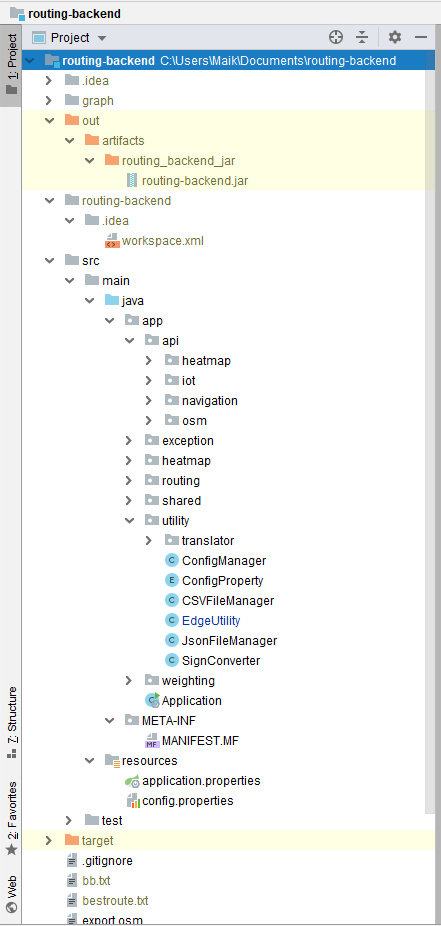
\includegraphics[width=8cm]{./ressourcen/routing/Ordnerstruktur-Routing.png}
	\caption{Ordnerstruktur der Routing-Komponente}
	\label{fig:folderstructure-routing}
\end{figure}

\Fig{folderstructure-routing} zeigt die Orderstruktur der Routing-Komponente.
Hier ist zu sehen, dass das Projekt aus zwei Hauptordnern besteht.
Diese sind der \textit{Java} und der \textit{resources} Ordner.

In dem \textit{resources} Ordner befinden sich zwei Config Dateien, in denen unter anderem der Server-Port oder die anzusprechenden Endpunkte angegeben werden.

In dem \textit{Java} Ordner befinden sich die Metadaten (\textit{MEAT-INF}) für die JAR-Datei und der Quellcode der Anwendung (\textit{app}).
Der \textit{app} Ordner ist unterteilt in die verschiedenen Teilkomponenten des Routing-Backends.
Hierzu zählen die Schnittstellen (\textit{api}), der Heatmap-Service (\textit{heatmap}), der Routing-Service (\textit{routing}), die Gewichtungs-Komponente (\textit{weighting}), ein Ordner für die allgemeine Funktionalitäten die an verschiedenen Stellen benötigt werden ({\textit{utility}) und ein Ordner in dem sich alle Klassen befinden die als Datenobjekte genutzt werden (\textit{shared}).

In dem \textit{api} Ordner gibt es Schnittstellen zur IoT-Plattform (\textit{heatmap}).
Hierüber werden die benötigten Daten zur Berechnung einer Route bzw. einer Heatmap abgefragt.
Außerdem gibt es noch Endpunkte die für die verschiedenen Frontends bereitgestellt werden. Erstens gibt es Endpunkte für die Navigationsanwendung(\textit{navigation}) und zweitens Endpunkte für die Heatmap (\textit{heatmap}).

In den Ordnern \textit{heatmap} und \textit{routing} befinden sich jeweils die Klassen die für die Berechnung der Heatmap bzw. der Route zuständig sind.

Der \textit{utility} Ordner enthält verschiedene Klassen mit Funktionalitäten, die von allen anderen Komponenten im Routing-Backend genutzte werden können. 
Hierzu gehören zum Beispiel die Translator Klassen, welche den Input des Nutzers überprüfen und umwandeln. 

Im \textit{weighting} Ordner befinden sich alle Klassen die für die Gewichtung der Kanten während der Routen-Berechnung zuständig sind.

Der \textit{shared} Ordner enthält alle Klassen, die als Datenstruktur im Routing-Backend genutzt werden, wie z.B. eine Route oder eine Heatmap.

Abschließend gibt es noch den \textit{exception} Ordner. 
Hierin befindet sich die Customexception, die für Fehlerrückmeldung genutzt wird.

\subsection{Technologien}
In diesem Abschnitt werden die wichtigsten Technologien beschrieben, die für die Entwicklung des Routing-Backends genutzt wurden.

Als Programmiersprache wurde Java verwendet, da es dafür die meisten Frameworks für Routing Algorithmen hab und die Studenten am meisten Erfahrung mit Java hatten.

Für die Routen Berechnung wurde das Framework GraphHopper genutzt. Hierdurch wurde die Implementierung eines eigenen Routing Algorithmus unnötig, da GraphHopper bereits A-Stern, Bidirektionalen Dijakstra und Contraction Hirachy. GraphHopper wird detaillierter in Kapitel Grundlagen im Dokument 1 beschrieben.

Als Entwicklungsumgebung wurde IntelliJ IDEA verwendet. Hier hätte aber ebenso eine andere Entwicklungsumgebung verwendet werden. Mit Intellij hatte die Studenten die besten Erfahrungen gemacht.

Außerdem wurde Maven verwendet um die Dependencies des Projekts einfacher verwalten zu können.

\subsection{Steps to Code}
In diesem Abschnitt werden die Schritte beschrieben, die durchgeführt werden müssen, um den Quellcode zu erweitern.

\begin{enumerate}
	\item Installiere IntelliJ IDEA\footnote{\url{https://www.jetbrains.com/idea/download/\#section=windows}}.
	\item Lade das Projekt aus dem Repository\footnote{\url{https://git.swl.informatik.uni-oldenburg.de/projects/PGRIO/repos/routing-backend/browse}} herunter.
	 \item Starte die IntelliJ IDEA Entwicklungsumgebung und öffne das Projekt (Datei -> Öffnen -> Projekt auswählen)
\end{enumerate}
	 
Jetzt kann begonnen werden den Quellcode zu bearbeiten. 
Wurde neuer Quellcode implementiert und der Entwickler möchte die Anwendung lokal starten kann er dies tun indem er die Main-Methode der Klasse \textit{Application} im Ordner \textit{app} startet. Über Postman kann man das Routing-Backend dann explorativ testen.

\subsection{Steps to Deploy}
Soll eine neue Version des Routing-Backends auf dem Develop-System deployt werden, müssen folgende Schritte durchgeführt werden.

\begin{enumerate}
	\item Führe mit Maven die Operation \textit{package} aus. Im Ordner \textit{target} wird eine Jar-Datei erstellt, die in den weiteren Schritten genutzt wird.
	\item Logge dich via Putty\footnote{\url{https://www.putty.org/}} auf der Develop-VM\footnote{\url{pg-rio-routing-dvlp.informatik.uni-oldenburg.de}} ein.
	\item Starte WinSCP und melde dich hier ebenfalls auf der Develop-VM an.
	\item Stoppe die auf der VM laufende Anwendung.
	\item Kopiere die neue lokal erzeugte Jar-Datei mit WinSCP auf die VM und überschreibe somit die alte Jar-Datei.
	\item Starte anschließend die neue Jar-Datei auf der VM.
\end{enumerate}
\subsection{Code Konventionen}
Als Grundlage für die Code Konventionen wurde die offiziellen Konventionen von Oracle genommen, die sehr verbreitet sind.

\section{Frontend}
In diesem Kapitel wird die Entwicklerdokumentation für die Navigationsanwendung beschrieben. Diese fasst alle relevanten Informationen zusammen, die für die Weiterentwicklung der Navigationsanwendung nötig sind. 

\subsection{Programmbeschreibung}
Die Navigations-App stellt das Ergebnis emissionsarmer Routen in einer graphischen Anwendung. 
Aus dem Zwecke einer stetigen und mobilen Verfügbarkeit wurde die Darstellung der Routenplanung innerhalb einer mobilen Anwendung umgesetzt. 
Diese mobile Anwendung wurde in Form einer hybriden Applikation konzipiert. 
Aus diesem Grund kann die Basis der Entwicklung auf unterschiedliche mobile Betriebssysteme \textit{IOS} u. \textit{Android} ausgeführt werden. 
Dabei wird der Inhalt unter Berücksichtigung eines Responsive Design in der jeweiligen Auflösung des Smartphones angepasst. 
Im Weiteren wird die Entwicklung und das Konzept der Navigations-App in einer Entwicklungsdokumentation beschrieben. 
Dies dient zum gemeinsamen Verständnis aller internen sowie externen Projektbeteiligten. 
Unter Berücksichtigung dieser Beschreibung wird ein grundlegendes Wissen über die Webentwicklung vorausgesetzt.

\subsection{Rahmenbedingungen}
%Ist der Abschnitt notwendig? Die externen Abhängigkeiten, Lizenzen etc. sind eher wichtig 
Für die Entwicklung der Navigations-App werden lediglich zwei Instrumenten benötigt. 
Das erste Instrument ist der Arbeitsrechner. Dieser wird zur Konzeption und zur Entwicklung der Programmarchitektur sowie des Programmcodes benötigt. 
Das zweite Instrument ist ein Android-Smartphone (+Version), welches zur Ausführung und zur Prüfung der mobilen Applikation verwendet wird. 
Beide Instrumente wurden in der Entwicklungs- und Konzeptionsphase von dem Projektteam gestellt.

\subsection{Steps to Code}
In diesem Abschnitt wird das Vorgehen beschrieben, wie ein neuer Entwickler zum Projekt der Navigationsapplikation beitragen kann. Im Folgenden werden die erforderlichen Schritte aufgezählt: 
\begin{enumerate}
	\item Installieren Sie Git.
	\item Klonen Sie das Projekt-Repository : 
	\begin{itemize}
		\item https://git.swl.informatik.uni-oldenburg.de/projects/PGRIO/repos/navigations-app/
	\end{itemize}
	\item Installieren eine IDE. Wir verwenden Visual Studio Code.
	\item Installieren Sie node.js und npm
	\item Installieren Sie Ionic CLI
	\begin{itemize}
		\item \$ npm install -g ionic
	\end{itemize}
	\item Installieren Sie Angular + Ionic Framework.
	\begin{itemize}
		\item \$ npm install @ionic/angular@latest --save
	\end{itemize}
	\item  Installieren Sie Cordova.
	\begin{itemize}
		\item \$ npm install -g cordova
	\end{itemize}
	\item Installieren Sie die erforderlichen Bibliotheken.
	\begin{itemize}
		\item \$ npm install
	\end{itemize}
	\item Um die Anwendung auf dem Handy zu installieren, schließen Sie Ihr Mobiltelefon an den Computer und und führen Sie diese Befehl aus:
	\begin{itemize}
		\item \$ ionic cordova run android
	\end{itemize}
\end{enumerate}

\subsection{Technische Rahmenbedingungen}
%Der Abschnitt ist doch genau das gleiche/selbe wie der darüber
Die Entwickler der Navigations-App benutzten während der gesamten Entwicklungsphase überwiegend die ihnen zur Verfügung   stehende persönliche Hardware. 
Neben dem eigenen Computer braucht man auch ein mobiles Gerät, um die verschiedensten mobilen Funktionen, wie zum Beispiel Navigieren anhand einer Route, testen zu können.
\subsection{Namenskonvention}
%Der Abschnitt sollte eigentlich unter dem Abschnitt "Code Konventionen"
Zum Start der Implementierung hat sich das Projektteam auf eine einheitliche Code-Convention geeinigt. 
Diese Code-Convention wurde im Laufe des Projektes von jedem der Projektbeteiligten eigenhalten. 
Dabei wurden sich auf folgende Rahmenbedingungen geeinigt: 
\begin{itemize}
	\item Alle Bezeichnungen wie Variablen, Kommentare, Dateinamen und Funktionen werden sprechend in englischer Sprache beschrieben.
	\item Die Vergabe von Namen sollte unter Berücksichtigung der Hauptfunktion beschrieben werden.
	\item Der Standard \textit{tslint-ionic-rules} wird verwendet.
\end{itemize}

\subsection{Datenstruktur des Projektes}
Verwendete Dateien und Ordner der Navigations-App werden in folgenden Ausprägungen strukturiert. 
In erster Linie werden alle für das Projekt installierten Module in dem Ordner \textit{node\_modules} hinterlegt. 
Dieser Ordner dient der strukturierten Auführung von internen sowie externen Modulen. 
Sollten Module benötigt werden, können diese von der \textit{package.json} Konfigurationsdatei als Abhängigkeit neu importiert werden. 
In zweiter Linie werden in dem \textit{src} Ordner, Dateien wie die \textit{index.htm}l,\textit{main.ts} und \textit{global.css} aufgeführt. 
Primär wird die \textit{index.html} Datei für den Aufruf der mobilen Applikation verwendet. 
Diese Datei beinhaltet den Container zur Anzeige der gesamten Applikation. 
Neben dieser Startseite wird in der \textit{main.ts} Datei die initiale Logik zur Kompilierung der Applikation beschrieben. 
Zur Darstellung eines globalen und individuellen Designs kann die \textit{global.css} als CSS-Datei verwendet werden. 
Kombiniert werden diese Strukturen jedoch in dem \textit{app}Ordner. 
In diesem Ordner befindet sich die Implementierung der einzelnen Anzeigen \textit{Pages}, den Komponenten \textit{Components}, den Service-Strukturen \textit{Services} sowie den Datenmodellen \textit{Models}. 
Eine zugehörige \textit{app.component} Datei bringt dabei alle Strukturen für einen initialen Start der Applikation zusammen.
Für diese Komponente wie auch den anderen Komponenten gibt eine jeweils eine Template Datei \textit{HTML} sowie einen Datenkontext \textit{TypeScript}. 
Ergänzend zu jeder Komponente wird im Erstellungsprozess die \textit{spec.ts} Datei erstellt. 
Diese dient dem reinen Zweck eine Komponente auf Methoden zu testen.

\subsection{Funktionalität}
In diesem Abschnitt werden die Funktionen der Navigationsapp genauer betrachtet. Zum einen werden Funktionalitäten bezüglich der Karte in \ref{sec:navigation:kartenfunktionalitaet} und zum anderen die Funktionalitäten bezüglich der Navigation in \ref{sec:navigation:navigationsfunktionaliteaten} näher erläutert. 
\subsubsection{Kartenfunktionalität}
\label{sec:navigation:kartenfunktionalitaet}
In diesem Abschnitt werden die Funktionalitäten der Karte in der Navigationapplikation näher beschrieben. Im Folgenden wird auf die Karte, die Routenberechnung und Darstellung eingegangen. Außerdem werden die Funktionen der aktuellen Position, der Geosuche, dem Verlauf der gespeicherten Eingaben sowie die Heatmap erläutert. \newline
\textbf{Karte} \newline
Beim Start der Anwendung wird die Karte mit \textit{leaflet} geladen. 
\textit{leaflet} ist eine JavaScript-Bibliothek für mobile-freundliche interaktive Karten. 
Die Karte wird auf die aktuelle Position zentriert. 
Das Laden der Karte erfolgt in \textit{home.page.ts} im Unterverzeichnis \textit{home}.

\textbf{Routenberechnung und Darstellung} \newline
Wenn Sie auf die Schaltfläche \textit{Route berechnen} klicken, wird die Funktion \textit{generateRoute()} aufgerufen. 
Die Funktion \textit{generateRoute()} befindet sich in \textit{route.component.ts} im Unterverzeichnis \textit{route}. 
Die Funktion \textit{generateRoute()} prüft, ob die Routenpunkte gültig sind, und sendet eine Anfrage an den Routingdienst, um eine Route zu berechnen. 
Beim Empfang der Routen wird die Funktion \textit{addRoute()} ausgelöst, um sie auf der Karte darzustellen. 
Die Funktion \textit{addRoute()} befindet sich in \textit{home.page.ts} im Unterverzeichnis \textit{home}.

\textbf{Aktuelle Position}\newline
Die aktuelle Position wird über den \textit{PositionService} bereitgestellt, der sich in \textit{position.service.ts} im Unterverzeichnis \textit{route} befindet. 
Der \textit{PositionService} verwendet das Ionic Native Plugin \textit{Geolocation}, um die aktuelle Position des Geräts zu überwachen.

\textbf{Geosuche} \newline
Beim tippen auf die Start, Zwischenziel oder Ziel eingabe wird jeweils \textit{doSearchStart()}, \textit{doSearch()}, \textit{doSearchInterim()} aufgerufen. 
Diese Funktionen finden Sie in \textit{route.component.ts} im Unterverzeichnis \textit{route}. 
Diese Funktionen führen die GeoSuche nach der eingegebenen Textadresse durch. 
Die Geosuche wird mit \textit{OpenStreetMapProvider} durchgeführt, der aus dem Plugin \textit{leaflet-geosearch} stammt.

\textbf{Verlauf gespeicherter Eingaben}\newline 
\begin{itemize}
	\item Beim Tippen auf das Start-, Zwischenziel- oder Ziel Eingabefeld wird die \textit{loadItems()} Funktion aufgerufen, um den gespeicherten Verlauf von Adrees mit Hilfe des \textit{storageService} abzurufen.
	
	\item Wenn Sie eine Adresse in das Eingabefeld start, Zwischenziel oder Ziel eingeben, wird die Funktion \textit{addItem()} aufgerufen, um die Adresse mithilfe des \textit{storageService} zu speichern.
	
	\item Wenn Sie auf das Löschsymbol neben einem Adressbuch der Verlaufsliste tippen, wird die Funktion \textit{deleteItem()} aufgerufen, um die Adresse mit dem \textit{storageService} aus dem gespeicherten Adressbuch zu löschen.
	
\end{itemize}
Die Funktionen \textit{addItem(), loadItems(), deleteItem()} befinden sich in \textit{route.component.ts} im Unterverzeichnis \textit{route}. 
Der \textit{storageService} befindet sich in \textit{storage.service.ts} im Unterverzeichnis \textit{services}.

\textbf{Feinstaubanzeige durch Heatmap}\newline
Wenn Sie auf die Heatmap-Schaltfläche tippen, wird die Funktion \textit{showHeatmap()} aufgerufen. 
Die Funktion \textit{showHeatmap()} befindet sich in \textit{home.page.ts} im Unterverzeichnis \textit{home}. 
\textit{showHeatmap()} hat ein Intervall von \textit{300} ms. in diesem intervall wird die Anfrage an den heatmap service gesendet. 
Beim Empfangen der Heatmap wird diese als neue Ebene auf der Karte mit Hilfe von \textit{leaflet-heatmap} Plugin gerendert.

\subsubsection{Navigation Funktionalität}
\label{sec:navigation:navigationsfunktionaliteaten}
In diesem Abschnitt werden die Funktionen der Navigation näher betrachtet. Dazu zählen der Navigationsalgorithmus sowie das dynamische Routing und die Abbiegehinweise. \newline
\textbf{Navigationsalgorithmus}\newline
beim Tippen auf die Navigationstaste wird die Funktion \textit{startNavigation()} aufgerufen. 
Die Funktion \textit{startNavigation()} befindet sich in \textit{home.page.ts} im Unterverzeichnis \textit{home}. 
Diese Funktion behält die ausgewählte Route bei, entfernt die anderen Routen, ruft die \textit{navigationAlgorithm()} Funktion zum Navigieren auf der ausgewählten Route auf und startet das dynamische Routing. 
Der \textit{navigationAlgorithm()} hat ein Intervall von 500 ms. 
In diesem Intervall wird die aktuelle Position mit den Abschnitten der gewählten Route verglichen, um festzustellen, auf welchem Abschnitt die aktuelle Position ist. 
Die aktuelle Position befindet sich auf einem Segment, wenn der Abstand zwischen der aktuellen Position und dem Segment kleiner als 15 Meter ist. 
Wenn sich die aktuelle Position auf einem Segment befindet, gilt Folgendes:
\begin{itemize}
	\item Die Abbiegeanweisung wird angezeigt.
	\item Der Abstand zum Ende des Segments wird berechnet.
	\item Der übergebene Teil des Segments wird grau dargestellt.
\end{itemize}

\textbf{Dynamisches Routing} \newline
Die Funktion \textit{startNavigation()} ruft die Funktion \textit{reRoute()} auf, um das dynamische Routing zu starten. 
Diese Funktion verfügt über ein Intervall, das über das Eingabefeld \textit{Zeitintervall} eingestellt wird. 
In diesem Intervall wird eine Anfrage an den Routing-Dienst gesendet, um eine Route zwischen der aktuellen Position und dem Ziel zu berechnen. 
Wenn sich diese neue Route von dem verbleibenden Teil der aktuell gefahrenen Route unterscheidet, wird diese neue Route als aktive Route festgelegt und zum Navigieren verwendet.

\textbf{Abbiegehinweise Liste} \newline
Wenn Sie auf die Anweisung für eine einzige Abbiegung tippen, wird die Liste aller Anweisungen für die Abbiegung angezeigt. 
Die Ansicht und die Logik dieser Liste finden Sie im \textit{tturnsinfo} Unterverzeichnis. 
In \textit{Turnsinfo.page.ts} wird auf der aktiven Route iteriert, um die Turn-Anweisungen zu extrahieren und in die Liste zu laden.

%Der Abschnitt für Code-Konventionen sollte noch eingefügt werden, da ihr ja auch ein tslint verwendet habt; siehe dafür Abschnitt Namenskonventionen

 




\cleardoublepage
% Phantomabsatz, damit die Seitenzahl im Pdf-Betrachter stimmt. (Wird von hyperref benötigt)
\phantomsection
\pagenumbering{Roman}
\setcounter{page}{\thecounterListPage}
% \nocite{*} % Für finales Dokument entfernen
\printbibliography

\cleardoublepage
% Phantomabsatz, damit die Seitenzahl im Pdf-Betrachter stimmt. (Wird von hyperref benötigt)
\phantomsection
% Glossar


\cleardoublepage
% Phantomabsatz, damit die Seitenzahl im Pdf-Betrachter stimmt. (Wird von hyperref benötigt)
\phantomsection
\pagenumbering{roman}
\appendix
% Anhang
\chapter{Anhang}


\section{Tabellen}

	\begin{table}[htb]
	\caption{Repositorien der IoT-Plattform und ihr Zweck}
	\begin{tabular}{|p{45mm}|p{93mm}|}
		\hline
		Name & Zweck \\ \hline
		iot"=api"=prototyp & Prototyp der IoT-Plattform, die im Rahmen des \schit entwickelt wurde (veraltet) \\ \hline
		iot"=api"=gateway & Zentrale Anlaufstelle für Anfragen von externen Diensten \\ \hline
		iot"=collection"=creater & Beinhaltet ein Skript zum Anlegen der MongoDB Collections mit den dazugehörigen Validierungsregeln \\ \hline
		iot"=data"=collector & Zentraler Dienst zum Sammeln der Daten (Messdaten, Konfigurationsdateien, usw.) vom MQTT Broker \\ \hline
		iot"=deployment"=skripte & Enthält Docker Compose Dateien und beispielhafte Konfigurationsdateien zum Bereitstellen der IoT-Plattform in jeglicher Umgebung \\ \hline
		iot"=hivemq"=extensions & Enthält Erweiterung für den verwendeten MQTT Broker HiveMQ, z.B. Authentifizierungs- und Autorisierungserweiterung \\ \hline
		iot"=identity"=service & Zentrale Authentifizierungsstelle für Microservices, externen API Nutzern oder MQTT Klienten. \\ \hline
		iot"=microservice"=humidity & Microservice für das Abfragen von gemessenen Luftfeuchte-Werten \\ \hline
		iot"=microservice"=pm10 & Microservice für das Abfragen von gemessenen PM10-Werten \\ \hline
		iot"=microservice"=pm25 & Microservice für das Abfragen von gemessenen PM25-Werten \\ \hline
		iot"=microservice"=pressure & Microservice für das Abfragen von gemessenen Luftdruck-Werten \\ \hline
		iot"=microservice"=sv & Microservice für die Funktionen der Sensorknotenverwaltungsoberfläche \\ \hline
		iot"=microservice"=temp & Microservice für das Abfragen von gemessenen Temperatur-Werten \\ \hline
		iot"=microservice"=template & Vorlage für das Erstellen neuer Microservices \\ \hline
		iot"=microservice"=uis & Microservice für die Funktionen der UIS Nutzeroberfläche \\ \hline
		iot"=mqtt"=broker"=hive & Ein Fork des HiveMQ Brokers mit den nötigen Erweiterungen \\ \hline
	\end{tabular}
	\label{tbl:iotrepos}
\end{table}

\begin{landscape}
	


\begin{table}[htb]
	\caption{Externe Abhängigkeiten der \skfw mit Links und Lizenzen}
	\begin{tabular}{|p{0.18\linewidth}|p{0.06\linewidth}|p{0.34\linewidth}|p{0.33\linewidth}|}
		\hline
		Name & Lizenz & Erläuterung & Weblink \\ \hline
		esp8266 & LGPL & Enthält Core-Funktionalitäten für den ESP8266. & \small\url{https://github.com/esp8266/Arduino} \\ \hline
		Esp""Software""Serial & LGPL & Erweitert die Core-Funktionalitäten für den ESP8266 um eine Software-basierte serielle Schnittstelle. & \url{https://github.com/plerup/espsoftwaerserial} \\ \hline
		make""Esp""Arduino & LGPL 2.1 & Enthält ein Make-File für den ESP8266. & \small\url{https://github.com/plerup/makeEspArduino} \\ \hline
		SparkFun BME""280 Arduino Library & MIT & Enthält Arduino-Library für den BME280. & \small\url{https://github.com/sparkfun/SparkFun_BME280_Arduino_Library} \\ \hline
		pubsubclient & MIT & Enthält Arduino-Client für MQTT. & \small\url{https://github.com/knolleary/pubsubclient} \\ \hline
		libserial & MIT & Enthält Funktionalität zur Kommunikation via serielle Schnittstelle auf Linux-Systemen. & \small\url{https://github.com/wjwwood/serial} \\ \hline
		paho.mqtt.c & EPL, EDL & Enthält Funktionalitäten zur Kommunikation via MQTT. Wird von paho.mqtt.cpp benötigt. & \small\url{https://github.com/eclipse/paho.mqtt.c} \\ \hline
		paho.mqtt.cpp & EPL, EDL & Enthält Client für MQTT unter Linux. & \small\url{https://github.com/eclipse/paho.mqtt.cpp} \\ \hline
		ArduinoJSON & MIT & Enthält Funktionalitäten zum Schreiben und Lesen von JSON"=Objekten. & \url{https://github.com/bblanchon/ArduinoJson} \\ \hline
		googletest & BSD3 & Unittest-Framework mit Testrunner. & \small\url{https://github.com/google/googletest} \\ \hline
		Fakeit & MIT & Mocking-Framework für Unittests. & \small\url{https://github.com/eranpeer/FakeIt} \\ \hline
	\end{tabular}
	\label{tbl:skextfwfull}
\end{table}

\begin{table}[htb]
	\caption{Lizenzen in der \skfw}
	\begin{tabular}{|p{0.06\linewidth}|p{0.34\linewidth}|p{0.53\linewidth}|}
		\hline
		Kürzel & Lizenz & Weblink \\ \hline
		LGPL 2.1 & GNU Lesser General Public License, version 2.1 & \url{https://www.gnu.org/licenses/old-licenses/lgpl-2.1.en.html} \\ \hline
		MIT & The MIT License & \url{https://mit-license.org/} \\ \hline
		EPL & Eclipse Public License - v 1.0 & \url{http://www.eclipse.org/legal/epl-v10.html} \\ \hline
		EDL & Eclipse Distribution License - v 1.0 & \url{http://www.eclipse.org/org/documents/edl-v10.php} \\ \hline
		BSD3 & The 3-Clause BSD License & \url{https://opensource.org/licenses/BSD-3-Clause} \\ \hline
	\end{tabular}
	\label{tbl:sklicenses}
\end{table}

\begin{table}[htb]
	\caption{Externe Abhängigkeiten iot"=api"=gateway mit Links und Lizenzen}
	\begin{tabular}{|p{0.18\linewidth}|p{0.06\linewidth}|p{0.06\linewidth}|p{0.28\linewidth}|p{0.33\linewidth}|}
		\hline
		Name & Version & Lizenz & Erläuterung & Weblink \\ \hline
		@nestjs/common & 6.0.0 & MIT & Benötigt für NestJS & \small\url{https://www.npmjs.com/package/@nestjs/common} \\ \hline
		@nestjs/core & 6.0.0 & MIT & Benötigt für NestJS & \small\url{https://www.npmjs.com/package/@nestjs/core} \\ \hline
		@nestjs/jwt & 6.0.0 & MIT & Benötigt für JWT in NestJS & \small\url{https://www.npmjs.com/package/@nestjs/jwt} \\ \hline
		@nestjs/mongoose & 6.1.2 & MIT & Benötigt für mongoose in NestJS & \small\url{https://www.npmjs.com/package/@nestjs/mongoose} \\ \hline
		@nestjs/platform-express & 6.0.0 & MIT & Benötigt für NestJS mit ExpressJS & \small\url{https://www.npmjs.com/package/@nestjs/platform-express} \\ \hline
		@nestjs/swagger & 3.0.2 & MIT & Benötigt für Swagger Dokumentation in NestJS & \small\url{https://www.npmjs.com/package/@nestjs/swagger} \\ \hline
		dotenv & 7.0.0 & BSD-2-Clause & Benötigt für das Laden von .env Konfigurationsdateien & \small\url{https://www.npmjs.com/package/dotenv} \\ \hline
		joi & 14.3.1 & BSD-3-Clause & Benötigt zum Validieren der Konfigurationsdateien & \small\url{https://www.npmjs.com/package/joi} \\ \hline
		mongoose & 5.6.11 & MIT & Benötigt zum Verbinden zur MongoDB & \small\url{https://www.npmjs.com/package/mongoose} \\ \hline
		request & 2.88.0 & Apache-2.0 & Benötigt für HTTP Requests zu den Microservices & \small\url{https://www.npmjs.com/package/request} \\ \hline
		request-promise-native & 1.0.7 & ISC & Wrapper zum Nutzen von nativen Promises bei HTTP Requests & \small\url{https://www.npmjs.com/package/request-promise-native} \\ \hline
		uuid & 3.3.2 & MIT & Generierung von einzigartigen IDs & \small\url{https://www.npmjs.com/package/uuid} \\ \hline
	\end{tabular}
	\label{tbl:dependenciesApiGateway}
\end{table}

\begin{table}[htb]
	\caption{Externe Abhängigkeiten iot"=collection"=creater mit Links und Lizenzen}
	\begin{tabular}{|p{0.18\linewidth}|p{0.06\linewidth}|p{0.06\linewidth}|p{0.28\linewidth}|p{0.33\linewidth}|}
		\hline
		Name & Version & Lizenz & Erläuterung & Weblink \\ \hline
		mongoose & 5.5.7 & MIT & Benötigt zum Verbinden zur MongoDB & \small\url{https://www.npmjs.com/package/mongoose} \\ \hline
		dotenv & 8.0.0 & BSD-2-Clause & Benötigt für das Laden von .env Konfigurationsdateien & \small\url{https://www.npmjs.com/package/dotenv} \\ \hline
		@hapi/joi & 15.0.2 & BSD-3-Clause & Benötigt zum Validieren der Konfigurationsdateien & \small\url{https://www.npmjs.com/package/@hapi/joi} \\ \hline
	\end{tabular}
	\label{tbl:dependenciesCollectionCreater}
\end{table}

\begin{table}[htb]
	\caption{Externe Abhängigkeiten iot"=data"=collector mit Links und Lizenzen}
	\begin{tabular}{|p{0.18\linewidth}|p{0.06\linewidth}|p{0.06\linewidth}|p{0.28\linewidth}|p{0.33\linewidth}|}
		\hline
		Name & Version & Lizenz & Erläuterung & Weblink \\ \hline
		mongoose & 5.5.7 & MIT & Benötigt zum Verbinden zur MongoDB & \small\url{https://www.npmjs.com/package/mongoose} \\ \hline
		dotenv & 8.0.0 & BSD-2-Clause & Benötigt für das Laden von .env Konfigurationsdateien & \small\url{https://www.npmjs.com/package/dotenv} \\ \hline
		@hapi/joi & 15.0.2 & BSD-3-Clause & Benötigt zum Validieren der Konfigurationsdateien & \small\url{https://www.npmjs.com/package/@hapi/joi} \\ \hline
		mqtt & 2.18.8 & MIT & MQTT Client zur Nutzung eines MQTT Broker & \small\url{https://www.npmjs.com/package/mqtt} \\ \hline
		@mongoosejs/double & 0.1.2 & MIT & Nutzung des Double Datentyps für die MongoDB & \small\url{https://www.npmjs.com/package/@mongoosejs/double} \\ \hline
	\end{tabular}
	\label{tbl:dependenciesDataCollector}
\end{table}

\begin{table}[htb]
	\caption{Externe Abhängigkeiten iot"=identity"=service mit Links und Lizenzen}
	\begin{tabular}{|p{0.18\linewidth}|p{0.06\linewidth}|p{0.06\linewidth}|p{0.28\linewidth}|p{0.33\linewidth}|}
		\hline
		Name & Version & Lizenz & Erläuterung & Weblink \\ \hline
		@nestjs/common & 6.0.0 & MIT & Benötigt für NestJS & \small\url{https://www.npmjs.com/package/@nestjs/common} \\ \hline
		@nestjs/core & 6.0.0 & MIT & Benötigt für NestJS & \small\url{https://www.npmjs.com/package/@nestjs/core} \\ \hline
		@nestjs/mongoose & 6.1.2 & MIT & Benötigt für mongoose in NestJS & \small\url{https://www.npmjs.com/package/@nestjs/mongoose} \\ \hline
		@nestjs/platform-express & 6.0.0 & MIT & Benötigt für NestJS mit ExpressJS & \small\url{https://www.npmjs.com/package/@nestjs/platform-express} \\ \hline
		@nestjs/swagger & 3.0.2 & MIT & Benötigt für Swagger Dokumentation in NestJS & \small\url{https://www.npmjs.com/package/@nestjs/swagger} \\ \hline
		dotenv & 7.0.0 & BSD-2-Clause & Benötigt für das Laden von .env Konfigurationsdateien & \small\url{https://www.npmjs.com/package/dotenv} \\ \hline
		joi & 14.3.1 & BSD-3-Clause & Benötigt zum Validieren der Konfigurationsdateien & \small\url{https://www.npmjs.com/package/joi} \\ \hline
		mongoose & 5.6.11 & MIT & Benötigt zum Verbinden zur MongoDB & \small\url{https://www.npmjs.com/package/mongoose} \\ \hline
	\end{tabular}
	\label{tbl:dependenciesIdentityService}
\end{table}

\begin{table}[htb]
	\caption{Externe Abhängigkeiten iot"=microservice"=pm10 mit Links und Lizenzen}
	\begin{tabular}{|p{0.18\linewidth}|p{0.06\linewidth}|p{0.06\linewidth}|p{0.28\linewidth}|p{0.33\linewidth}|}
		\hline
		Name & Version & Lizenz & Erläuterung & Weblink \\ \hline
		@nestjs/common & 6.0.0 & MIT & Benötigt für NestJS & \small\url{https://www.npmjs.com/package/@nestjs/common} \\ \hline
		@nestjs/core & 6.0.0 & MIT & Benötigt für NestJS & \small\url{https://www.npmjs.com/package/@nestjs/core} \\ \hline
		@nestjs/mongoose & 6.1.2 & MIT & Benötigt für mongoose in NestJS & \small\url{https://www.npmjs.com/package/@nestjs/mongoose} \\ \hline
		@nestjs/platform-express & 6.0.0 & MIT & Benötigt für NestJS mit ExpressJS & \small\url{https://www.npmjs.com/package/@nestjs/platform-express} \\ \hline
		@nestjs/swagger & 3.0.2 & MIT & Benötigt für Swagger Dokumentation in NestJS & \small\url{https://www.npmjs.com/package/@nestjs/swagger} \\ \hline
		dotenv & 7.0.0 & BSD-2-Clause & Benötigt für das Laden von .env Konfigurationsdateien & \small\url{https://www.npmjs.com/package/dotenv} \\ \hline
		joi & 14.3.1 & BSD-3-Clause & Benötigt zum Validieren der Konfigurationsdateien & \small\url{https://www.npmjs.com/package/joi} \\ \hline
		mongoose & 5.6.11 & MIT & Benötigt zum Verbinden zur MongoDB & \small\url{https://www.npmjs.com/package/mongoose} \\ \hline
	\end{tabular}
	\label{tbl:dependenciesMicroPM10}
\end{table}

\begin{table}[htb]
	\caption{Externe Abhängigkeiten iot"=microservice"=pm25 mit Links und Lizenzen}
	\begin{tabular}{|p{0.18\linewidth}|p{0.06\linewidth}|p{0.06\linewidth}|p{0.28\linewidth}|p{0.33\linewidth}|}
		\hline
		Name & Version & Lizenz & Erläuterung & Weblink \\ \hline
		@nestjs/common & 6.0.0 & MIT & Benötigt für NestJS & \small\url{https://www.npmjs.com/package/@nestjs/common} \\ \hline
		@nestjs/core & 6.0.0 & MIT & Benötigt für NestJS & \small\url{https://www.npmjs.com/package/@nestjs/core} \\ \hline
		@nestjs/mongoose & 6.1.2 & MIT & Benötigt für mongoose in NestJS & \small\url{https://www.npmjs.com/package/@nestjs/mongoose} \\ \hline
		@nestjs/platform-express & 6.0.0 & MIT & Benötigt für NestJS mit ExpressJS & \small\url{https://www.npmjs.com/package/@nestjs/platform-express} \\ \hline
		@nestjs/swagger & 3.0.2 & MIT & Benötigt für Swagger Dokumentation in NestJS & \small\url{https://www.npmjs.com/package/@nestjs/swagger} \\ \hline
		dotenv & 7.0.0 & BSD-2-Clause & Benötigt für das Laden von .env Konfigurationsdateien & \small\url{https://www.npmjs.com/package/dotenv} \\ \hline
		joi & 14.3.1 & BSD-3-Clause & Benötigt zum Validieren der Konfigurationsdateien & \small\url{https://www.npmjs.com/package/joi} \\ \hline
		mongoose & 5.6.11 & MIT & Benötigt zum Verbinden zur MongoDB & \small\url{https://www.npmjs.com/package/mongoose} \\ \hline
	\end{tabular}
	\label{tbl:dependenciesMicroPM25}
\end{table}

\begin{table}[htb]
	\caption{Externe Abhängigkeiten iot"=microservice"=temp mit Links und Lizenzen}
	\begin{tabular}{|p{0.18\linewidth}|p{0.06\linewidth}|p{0.06\linewidth}|p{0.28\linewidth}|p{0.33\linewidth}|}
		\hline
		Name & Version & Lizenz & Erläuterung & Weblink \\ \hline
		@nestjs/common & 6.0.0 & MIT & Benötigt für NestJS & \small\url{https://www.npmjs.com/package/@nestjs/common} \\ \hline
		@nestjs/core & 6.0.0 & MIT & Benötigt für NestJS & \small\url{https://www.npmjs.com/package/@nestjs/core} \\ \hline
		@nestjs/mongoose & 6.1.2 & MIT & Benötigt für mongoose in NestJS & \small\url{https://www.npmjs.com/package/@nestjs/mongoose} \\ \hline
		@nestjs/platform-express & 6.0.0 & MIT & Benötigt für NestJS mit ExpressJS & \small\url{https://www.npmjs.com/package/@nestjs/platform-express} \\ \hline
		@nestjs/swagger & 3.0.2 & MIT & Benötigt für Swagger Dokumentation in NestJS & \small\url{https://www.npmjs.com/package/@nestjs/swagger} \\ \hline
		dotenv & 7.0.0 & BSD-2-Clause & Benötigt für das Laden von .env Konfigurationsdateien & \small\url{https://www.npmjs.com/package/dotenv} \\ \hline
		joi & 14.3.1 & BSD-3-Clause & Benötigt zum Validieren der Konfigurationsdateien & \small\url{https://www.npmjs.com/package/joi} \\ \hline
		mongoose & 5.6.11 & MIT & Benötigt zum Verbinden zur MongoDB & \small\url{https://www.npmjs.com/package/mongoose} \\ \hline
	\end{tabular}
	\label{tbl:dependenciesMicroTemp}
\end{table}

\begin{table}[htb]
	\caption{Externe Abhängigkeiten iot"=microservice"=sv mit Links und Lizenzen}
	\begin{tabular}{|p{0.18\linewidth}|p{0.06\linewidth}|p{0.06\linewidth}|p{0.28\linewidth}|p{0.33\linewidth}|}
		\hline
		Name & Version & Lizenz & Erläuterung & Weblink \\ \hline
		@nestjs/common & 6.0.0 & MIT & Benötigt für NestJS & \small\url{https://www.npmjs.com/package/@nestjs/common} \\ \hline
		@nestjs/core & 6.0.0 & MIT & Benötigt für NestJS & \small\url{https://www.npmjs.com/package/@nestjs/core} \\ \hline
		@nestjs/mongoose & 6.1.2 & MIT & Benötigt für mongoose in NestJS & \small\url{https://www.npmjs.com/package/@nestjs/mongoose} \\ \hline
		@nestjs/platform-express & 6.0.0 & MIT & Benötigt für NestJS mit ExpressJS & \small\url{https://www.npmjs.com/package/@nestjs/platform-express} \\ \hline
		@nestjs/swagger & 3.0.2 & MIT & Benötigt für Swagger Dokumentation in NestJS & \small\url{https://www.npmjs.com/package/@nestjs/swagger} \\ \hline
		dotenv & 7.0.0 & BSD-2-Clause & Benötigt für das Laden von .env Konfigurationsdateien & \small\url{https://www.npmjs.com/package/dotenv} \\ \hline
		joi & 14.3.1 & BSD-3-Clause & Benötigt zum Validieren der Konfigurationsdateien & \small\url{https://www.npmjs.com/package/joi} \\ \hline
		mongoose & 5.6.11 & MIT & Benötigt zum Verbinden zur MongoDB & \small\url{https://www.npmjs.com/package/mongoose} \\ \hline
		jwt-decode & 2.2.0 & MIT & Benötigt zum dekodieren von JWT & \small\url{https://www.npmjs.com/package/jwt-decode} \\ \hline
		mqtt & 3.0.0 & MIT & MQTT Client zur Nutzung eines MQTT Broker & \small\url{https://www.npmjs.com/package/mqtt} \\ \hline
	\end{tabular}
	\label{tbl:dependenciesMicroSV}
\end{table}

\begin{table}[htb]
	\caption{Externe Abhängigkeiten iot"=microservice"=uis mit Links und Lizenzen}
	\begin{tabular}{|p{0.18\linewidth}|p{0.06\linewidth}|p{0.06\linewidth}|p{0.28\linewidth}|p{0.33\linewidth}|}
		\hline
		Name & Version & Lizenz & Erläuterung & Weblink \\ \hline
		@nestjs/common & 6.0.0 & MIT & Benötigt für NestJS & \small\url{https://www.npmjs.com/package/@nestjs/common} \\ \hline
		@nestjs/core & 6.0.0 & MIT & Benötigt für NestJS & \small\url{https://www.npmjs.com/package/@nestjs/core} \\ \hline
		@nestjs/mongoose & 6.1.2 & MIT & Benötigt für mongoose in NestJS & \small\url{https://www.npmjs.com/package/@nestjs/mongoose} \\ \hline
		@nestjs/platform-express & 6.0.0 & MIT & Benötigt für NestJS mit ExpressJS & \small\url{https://www.npmjs.com/package/@nestjs/platform-express} \\ \hline
		@nestjs/swagger & 3.0.2 & MIT & Benötigt für Swagger Dokumentation in NestJS & \small\url{https://www.npmjs.com/package/@nestjs/swagger} \\ \hline
		dotenv & 7.0.0 & BSD-2-Clause & Benötigt für das Laden von .env Konfigurationsdateien & \small\url{https://www.npmjs.com/package/dotenv} \\ \hline
		joi & 14.3.1 & BSD-3-Clause & Benötigt zum Validieren der Konfigurationsdateien & \small\url{https://www.npmjs.com/package/joi} \\ \hline
		mongoose & 5.6.11 & MIT & Benötigt zum Verbinden zur MongoDB & \small\url{https://www.npmjs.com/package/mongoose} \\ \hline
		mqtt & 3.0.0 & MIT & MQTT Client zur Nutzung eines MQTT Broker & \small\url{https://www.npmjs.com/package/mqtt} \\ \hline
	\end{tabular}
	\label{tbl:dependenciesMicroUIS}
\end{table}

\end{landscape}



\end{document}
